% write your paper in here

\newcommand{\beginsupplement}{%
        \setcounter{table}{0}
        \renewcommand{\thetable}{S\arabic{table}}%
        \setcounter{figure}{0}
        \renewcommand{\thefigure}{S\arabic{figure}}%
     }

\chapter{Benchmark of long-read assemblers on the genome of the bdelloid rotifer \textit{Adineta vaga}}

Long reads have made highly contiguous assemblies accessible for all genomes, but most long-read assemblers aim to produce a haploid assembly, regardless of the actual degree of ploidy (haploid, diploid or polyploid) of the genome being assembled. To obtain haploid assemblies from diploid or polyploid genomes, homologous chromosomes need to be collapsed into a single sequence. This process is straightforward for homozygous regions, but more challenging for heterozygous regions as the assembler needs to find a consensus between haplotypes or select one to represent the region. Collapsing haplotypes is especially challenging for non-model diploid or polyploid genomes, as they often display variable levels of heterozygosity across their genomes. \\

Long-read assemblers have proven efficient at generating assemblies with high contiguity and completeness on low-heterozygosity genome, but they are rarely tested on non-model genomes, and it is unclear how well they can deal with higher levels of heterozygosity. To fill this gap, I designed a benchmark of seven long-read assemblers, namely Canu \cite{canu}, Flye \cite{flye}, NextDenovo \cite{nextdenovo}, Ra \cite{ra}, Raven \cite{raven}, Shasta \cite{shasta} and wtdbg2 \cite{wtdbg2}. I tested these assemblers on the genome of a non-model diploid organism, \textit{Adineta vaga}, for which high-coverage sequencing datasets of both Pacific Biosciences (PacBio) and Oxford Nanopore Technologies (Nanopore) low-accuracy long reads were available. I defined a thorough evaluation strategy to identify the best haploid assemblies, based on assembly size, contiguity, completeness, and a new metric of haploidy that was implemented in the tool HapPy. \\

I first focused on assemblies of the full PacBio or Nanopore datasets and I found that two assemblers, Ra and wtdbg2, produced contigs with less remaining uncollapsed haplotypes. Second, I assembled only a subset of reads, based on their length exclusively, or on both length and quality with Filtlong \cite{filtlong}. I found that this strategy could improve haplotype-collapsing for some assemblers, and increase contiguity and completeness. Third, I tested three haplotig-purging tools, HaploMerger2 \cite{haplomerger2}, purge\_dups \cite{purge_dups} and Purge Haplotigs \cite{purge_haplotigs}, to evaluate how well they could remove haplotigs and more generally how they would improve the assemblies. Finally, I tested together read filtering and/or haplotig-purging tools and found that combining read filtering and purge\_dups or purge\_haplotigs, or combining purge\_dups and purge\_haplotigs, could lead to assemblies with high contiguity, completeness, and reduced uncollapsed haplotypes. \\

I evaluated the impact of sequencing depth on haplotype collapsing and overall assembly quality. I found that most assemblers were optimized for a sequencing depth of 40X, and that a higher sequencing depth would not necessarily improve the assemblies but would rather lead to more uncollapsed haplotypes. \\

The end purpose of this benchmark is to provide users with a methodology to obtain haploid assemblies of non-model eukaryote organisms with high contiguity and completeness, and that suit their computational requirements. I initiated this benchmark to evaluate how long read assemblers behaved on a eukaryote genome, as there was only one benchmark available on bacteria. I used these strategies in several genome assembly projects to obtain properly collapsed haploid assemblies. \\

%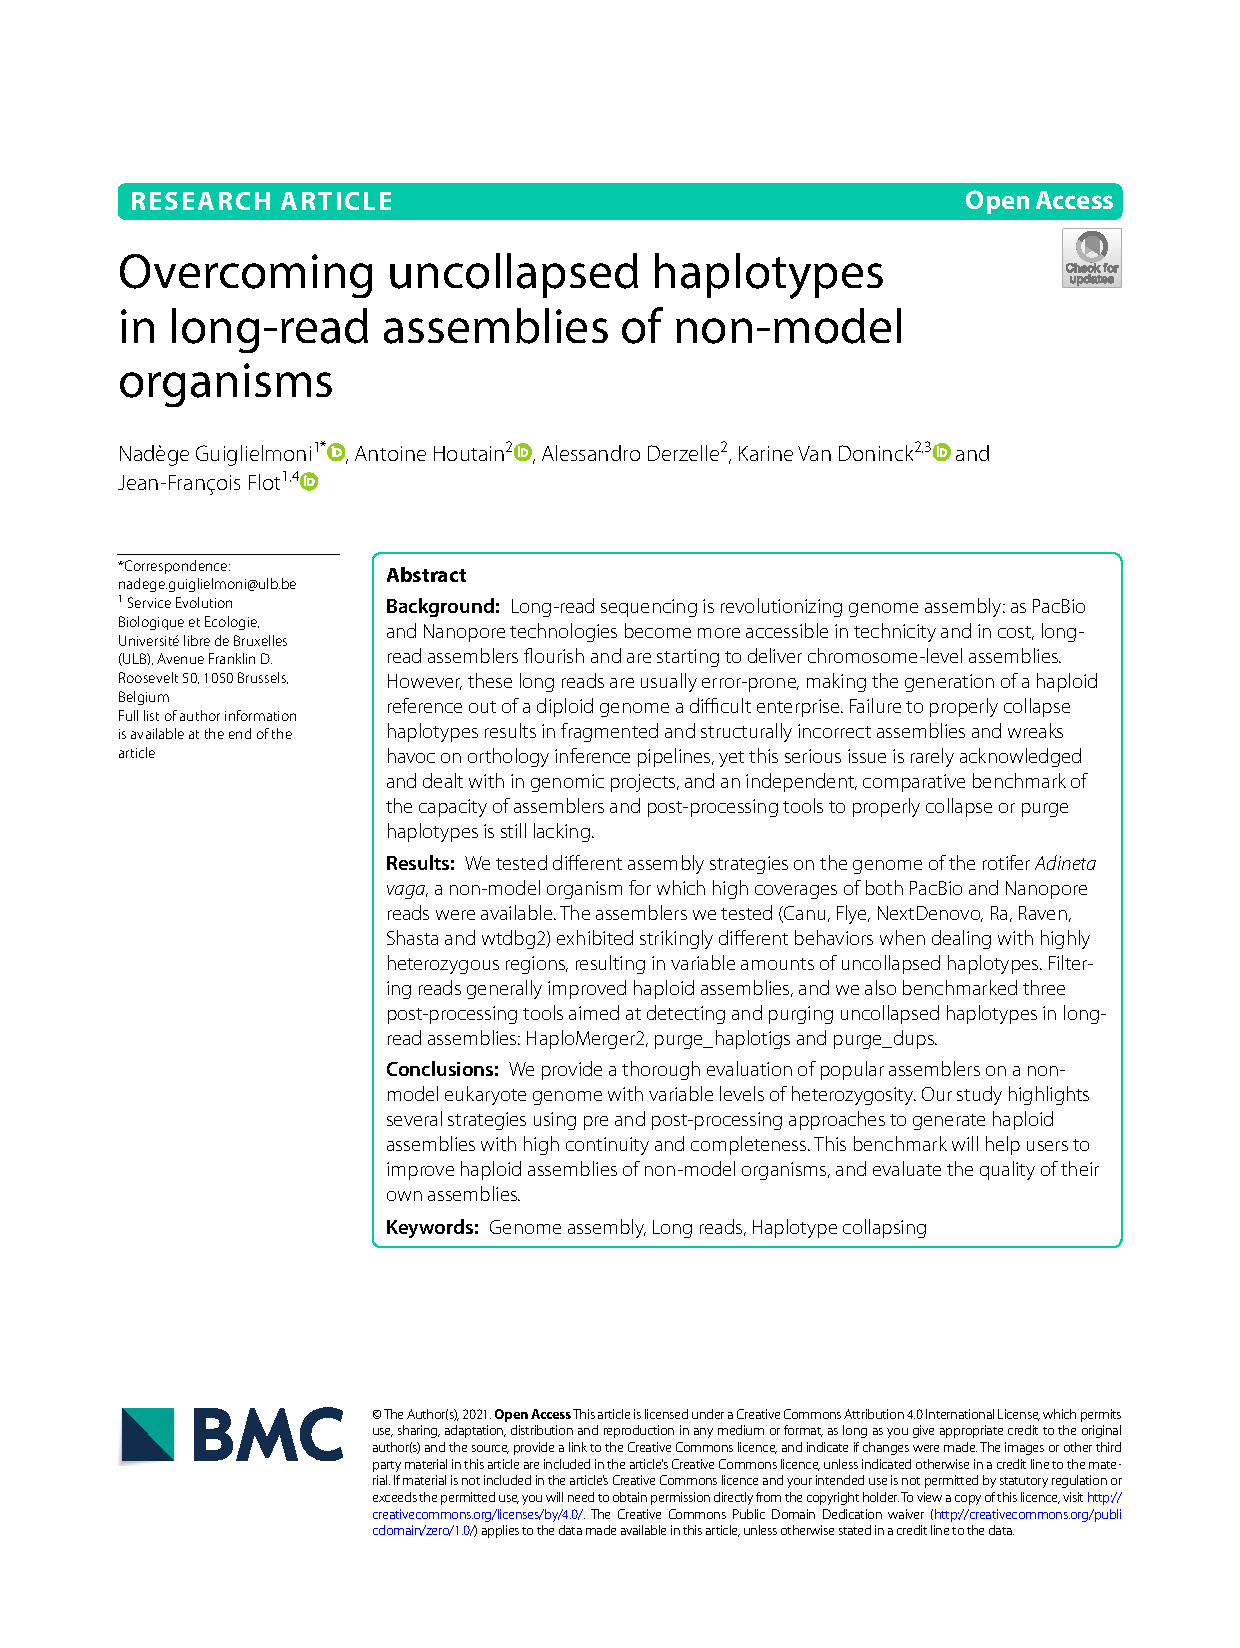
\includepdf[pages=-, pagecommand={}]{articles/benchmark.pdf}

\beginsupplement

\section*{Supplementary data}

   \begin{figure}[ht]
    \centering
     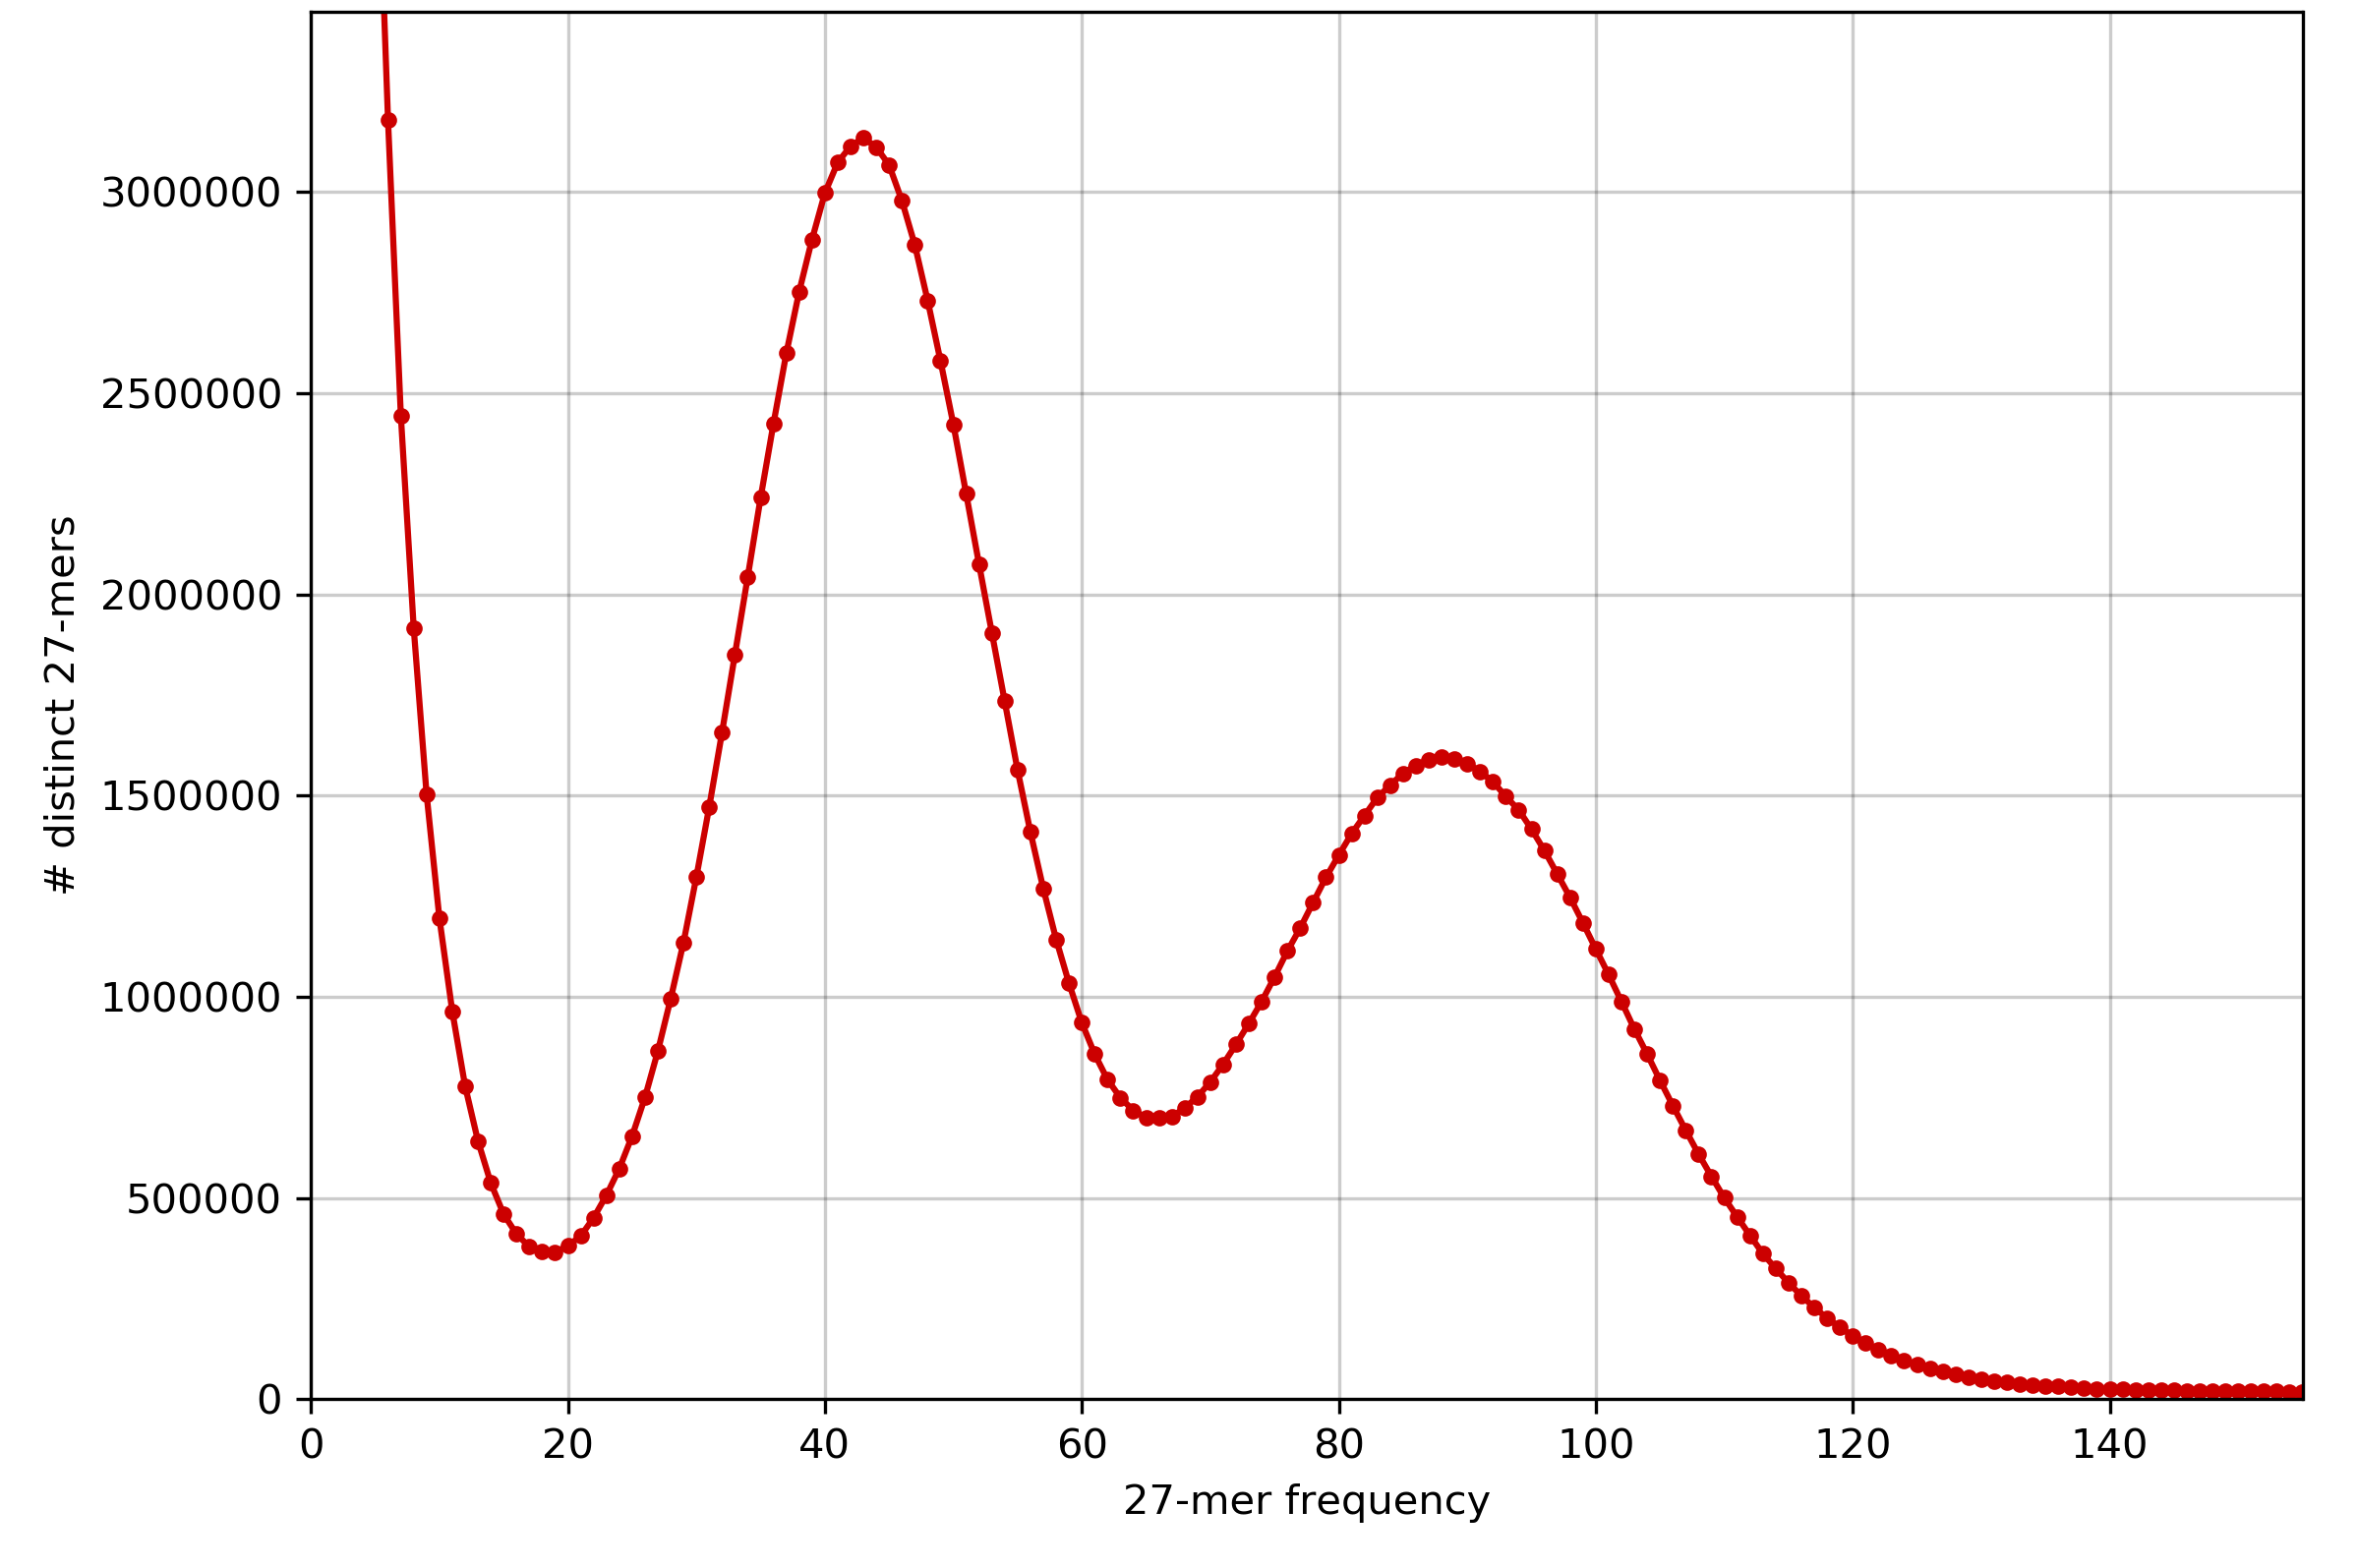
\includegraphics[width=13.5cm]{fig/benchmark/avaga_lab_kat.hist.png}
   \caption{\textit{k}-mer spectrum of \textit{Adineta vaga} using Illumina reads and KAT v2.4.2. The first peak corresponds to heterozygous \textit{k}-mers (around 45X) and the second peak corresponds to homozygous \textit{k}-mers.}
   \label{fig:kmer_spectrum}
 \end{figure}

   \begin{figure}[ht]
    \centering
     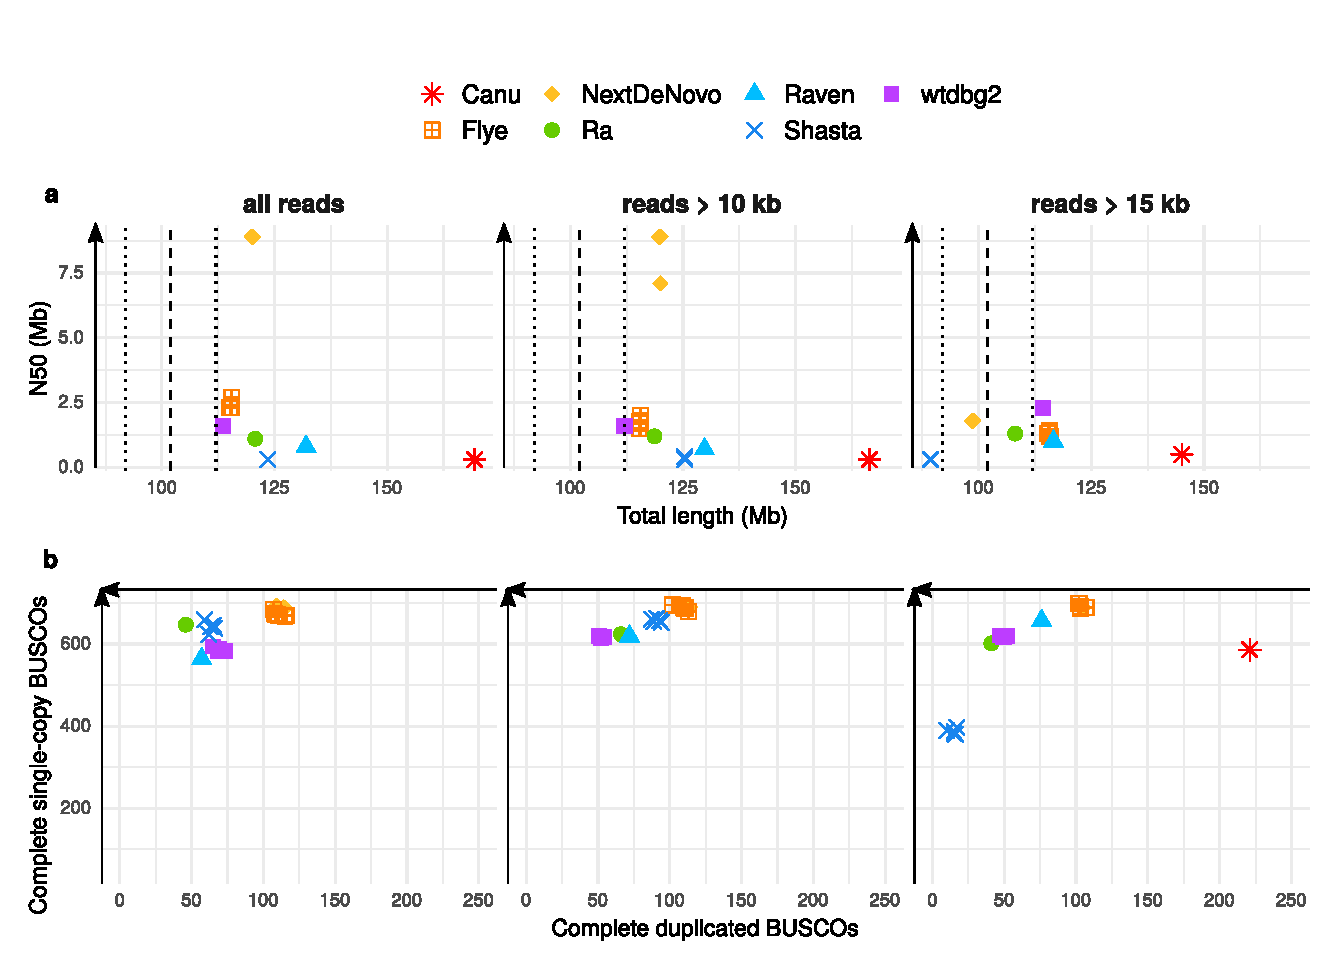
\includegraphics[width=13.5cm]{fig/benchmark/supp_pacbio_replicates.eps}
   \caption{Statistics of PacBio assemblies obtained from the full PacBio dataset or with a read-filtering step prior to assembly based on read length exclusively, using different thresholds: 10 kb, 15 kb. All assemblies were run five times to assess the reproducibility of the output produced by each assembler. a) N50 plotted against total assembly length. The dashed line indicates the expected genome size, with a +/- 10 Mb margin delimited by the dotted lines. b) Number of complete single-copy BUSCOs plotted against number of complete duplicated BUSCOs, from a total of 954 orthologs.}
   \label{fig:pacbio_replicates}
 \end{figure}
 
    \begin{figure}[ht]
    \centering
     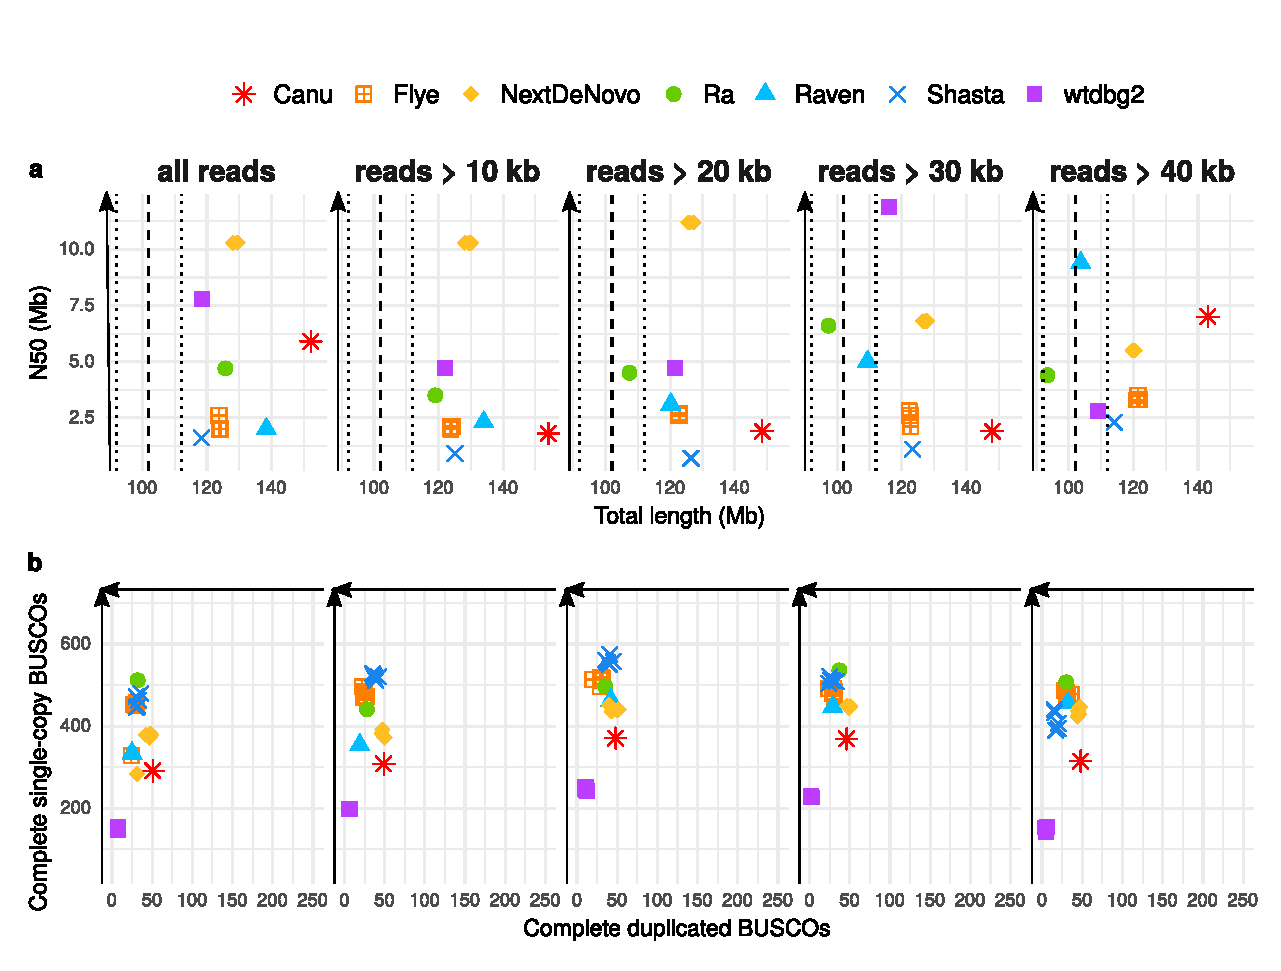
\includegraphics[width=13.5cm]{fig/benchmark/supp_nanopore_replicates.eps}
   \caption{Statistics of Nanopore assemblies obtained from the full Nanopore dataset or with a read-filtering step prior to assembly based on read length exclusively, using different thresholds: 10 kb, 20 kb, 30 kb, 40 kb. All assemblies were run five times to assess the reproducibility of the output produced by each assembler. a) N50 plotted against total assembly length. The dashed line indicates the expected genome size, with +/- 10 Mb margin delimited by the dotted lines. b) Number of complete single-copy BUSCOs plotted against number of complete duplicated BUSCOs, from a total of 954 orthologs.}
   \label{fig:nanopore_replicates}
 \end{figure}

   \begin{figure}[ht]
    \centering
     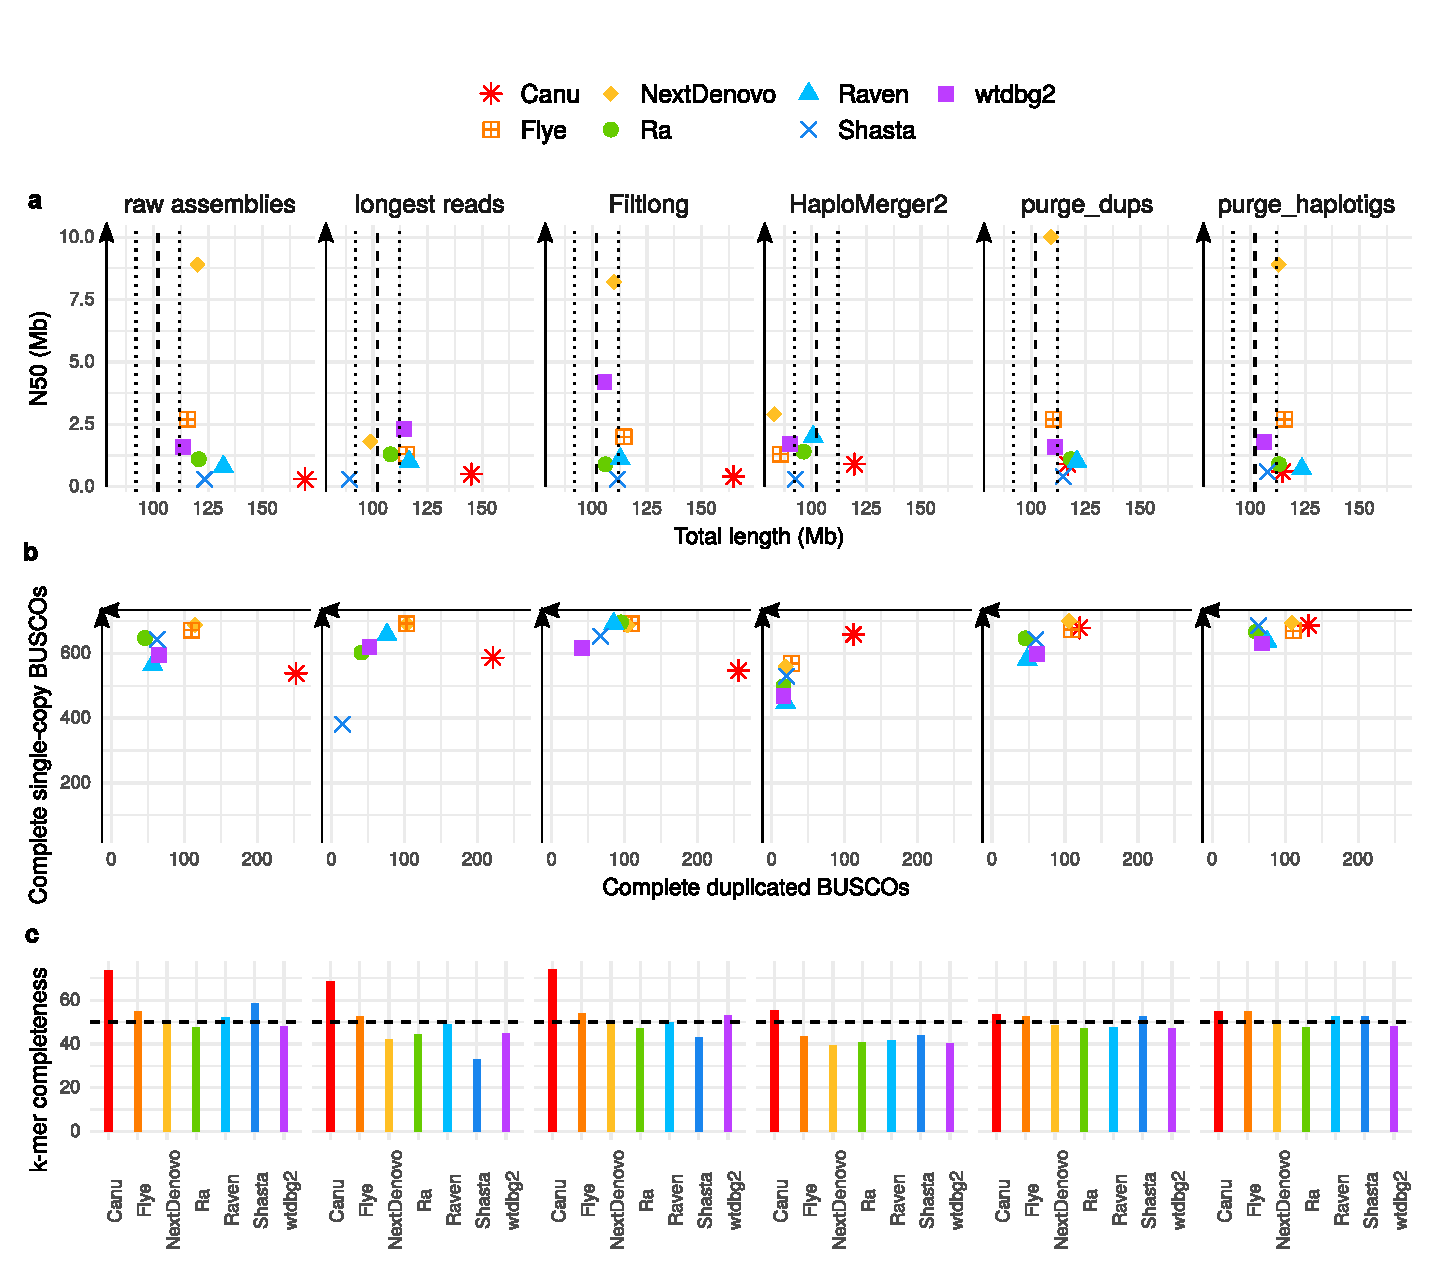
\includegraphics[width=13.5cm]{fig/benchmark/pacbio_all_v20210317.eps}
   \caption{Statistics of raw assemblies obtained from the full PacBio dataset (raw assemblies), with a preliminary read filtering step (keeping only reads larger than 15 kb, or those selected by Filtlong based on quality and length) or a subsequent removal of uncollapsed haplotypes with HaploMerger2, purge\_dups, or purge\_haplotigs. a) N50 plotted against total assembly length. The dashed line indicates the expected genome size, with +/- 10 Mb margin delimited by the dotted lines. b) Number of complete single-copy BUSCOs plotted against number of complete duplicated BUSCOs, from a total of 954 orthologs. c) \textit{k}-mer completeness. The dashed line indicates the expected 50\% completeness.}
   \label{fig:pacbio_full_stats}
 \end{figure}
 
  \begin{figure}[ht]
    \centering
     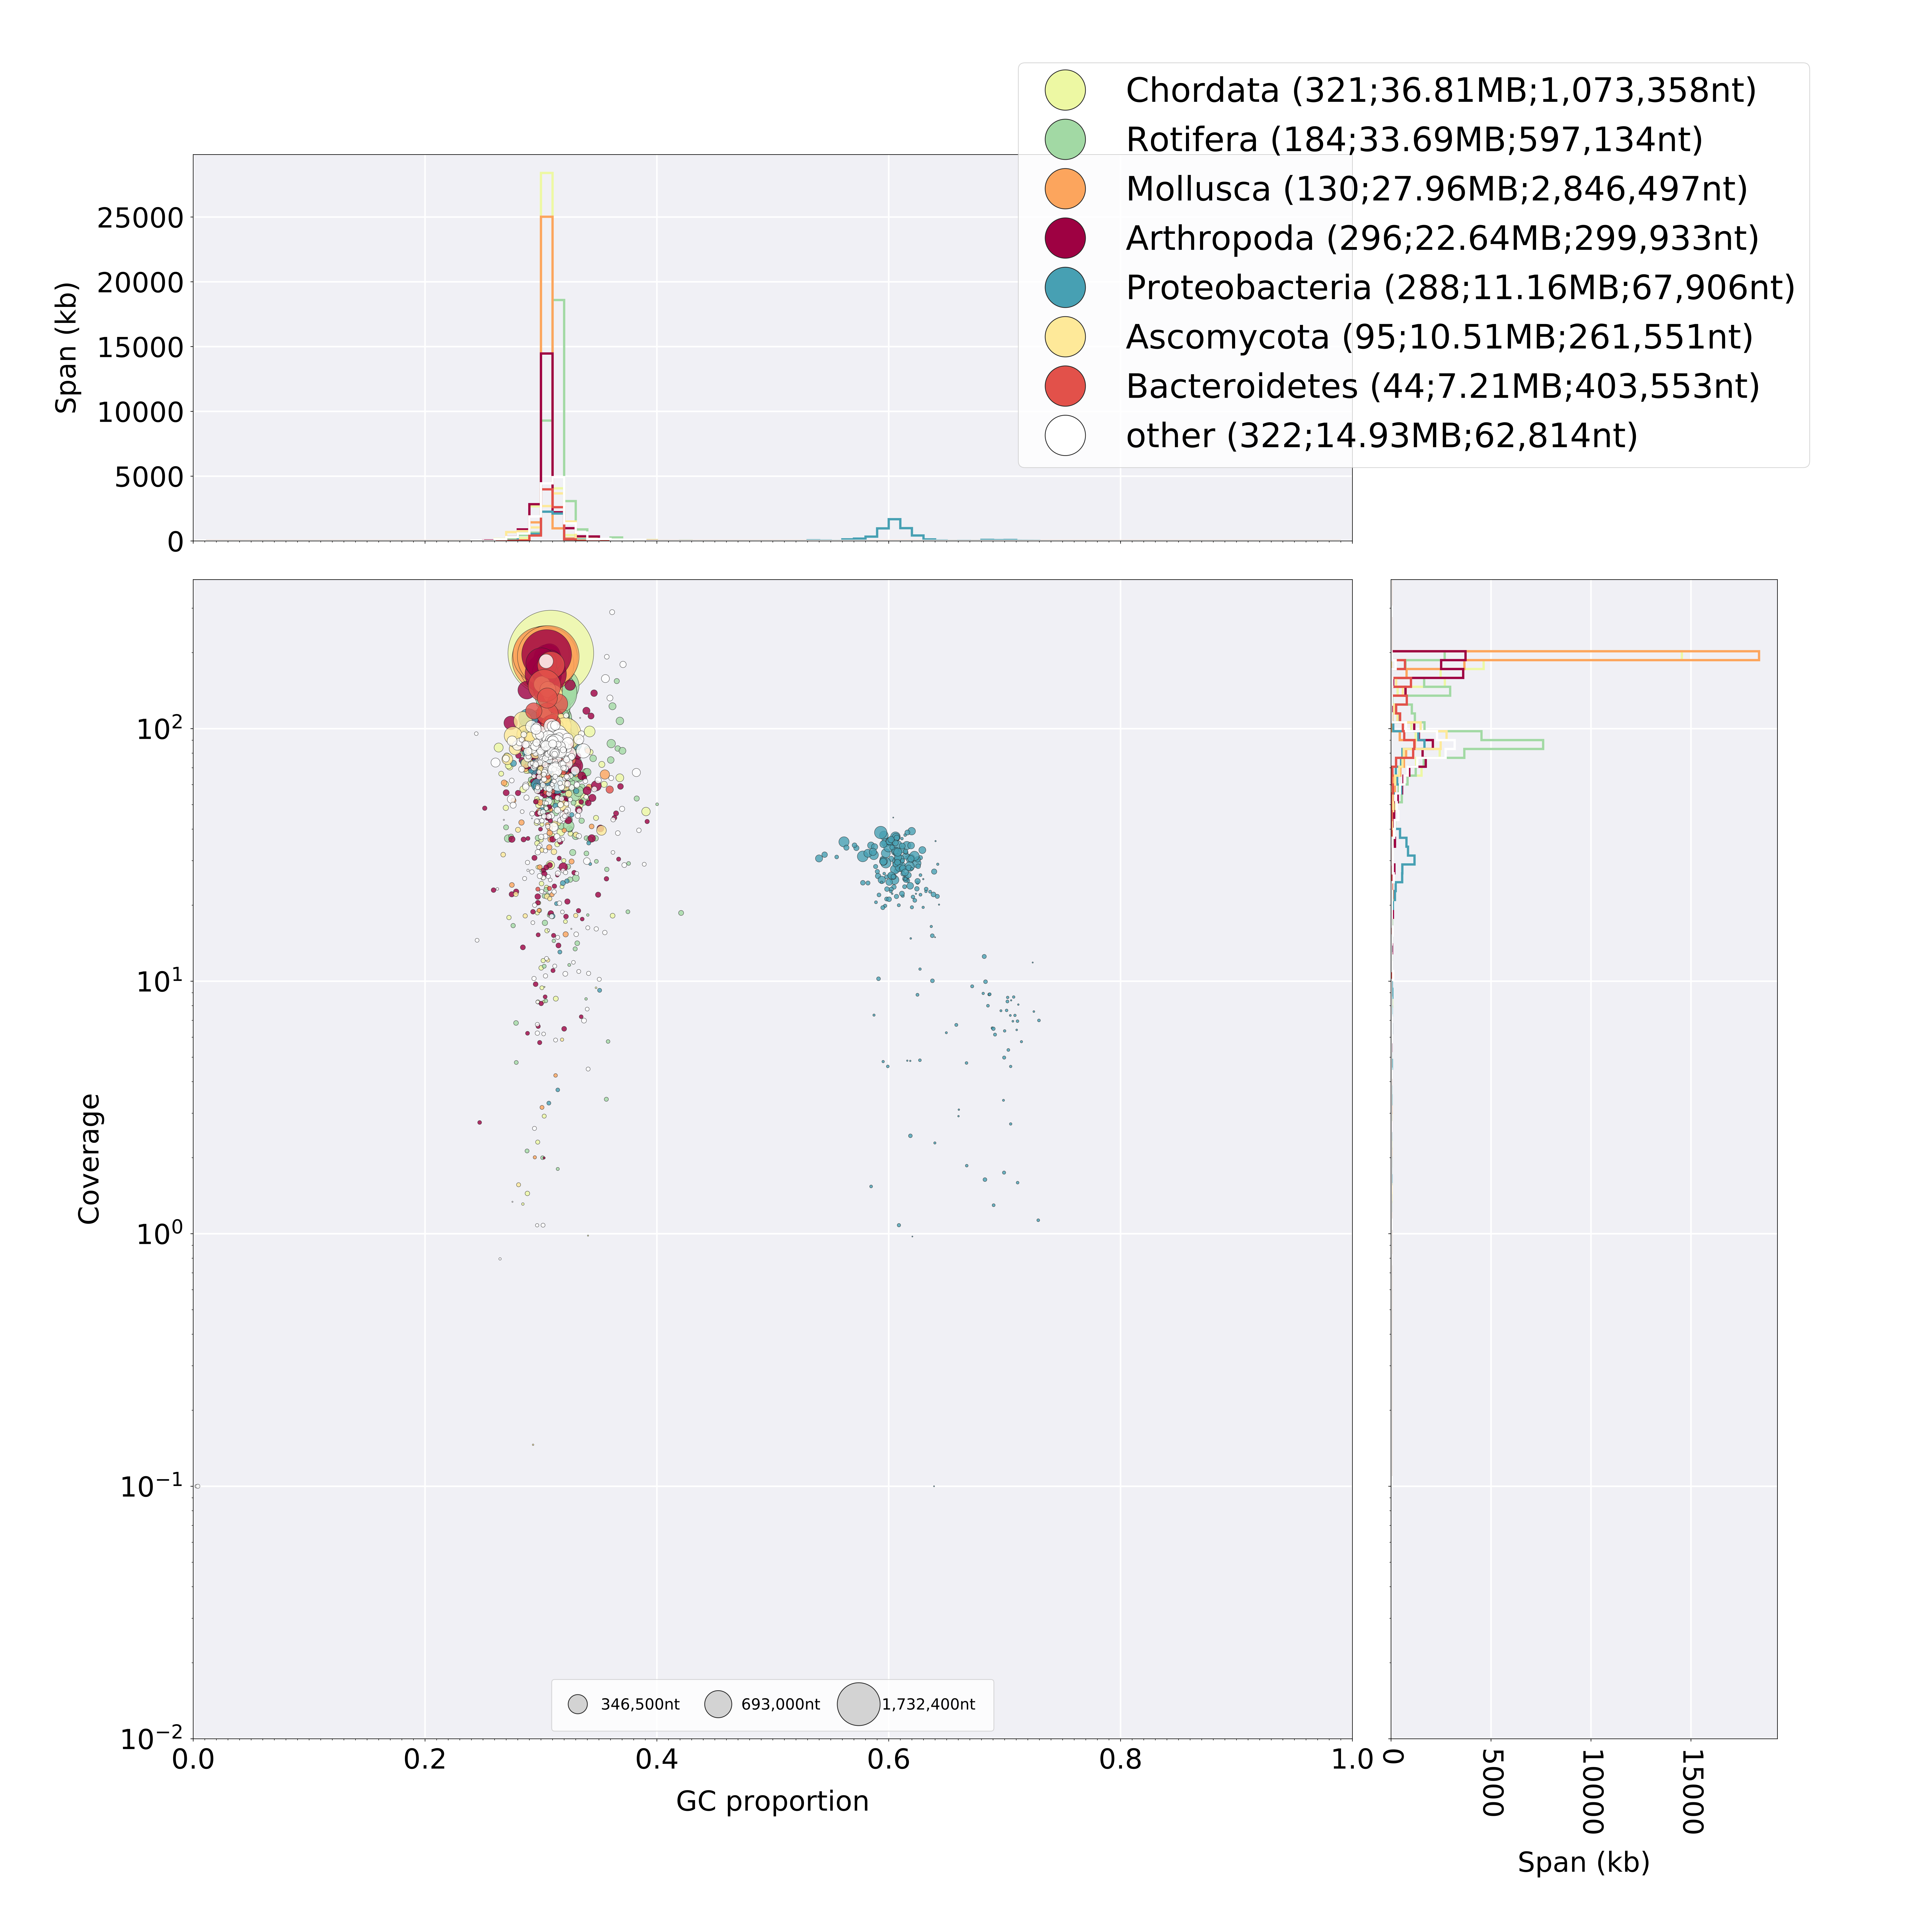
\includegraphics[width=15cm]{fig/benchmark/PB_CANU.png}
   \caption{Blobtools v1.0 analysis of a Canu assembly of the full PacBio dataset.}
   \label{fig:blobtools_canu_pb}
 \end{figure}
 
 \begin{figure}[ht]
    \centering
     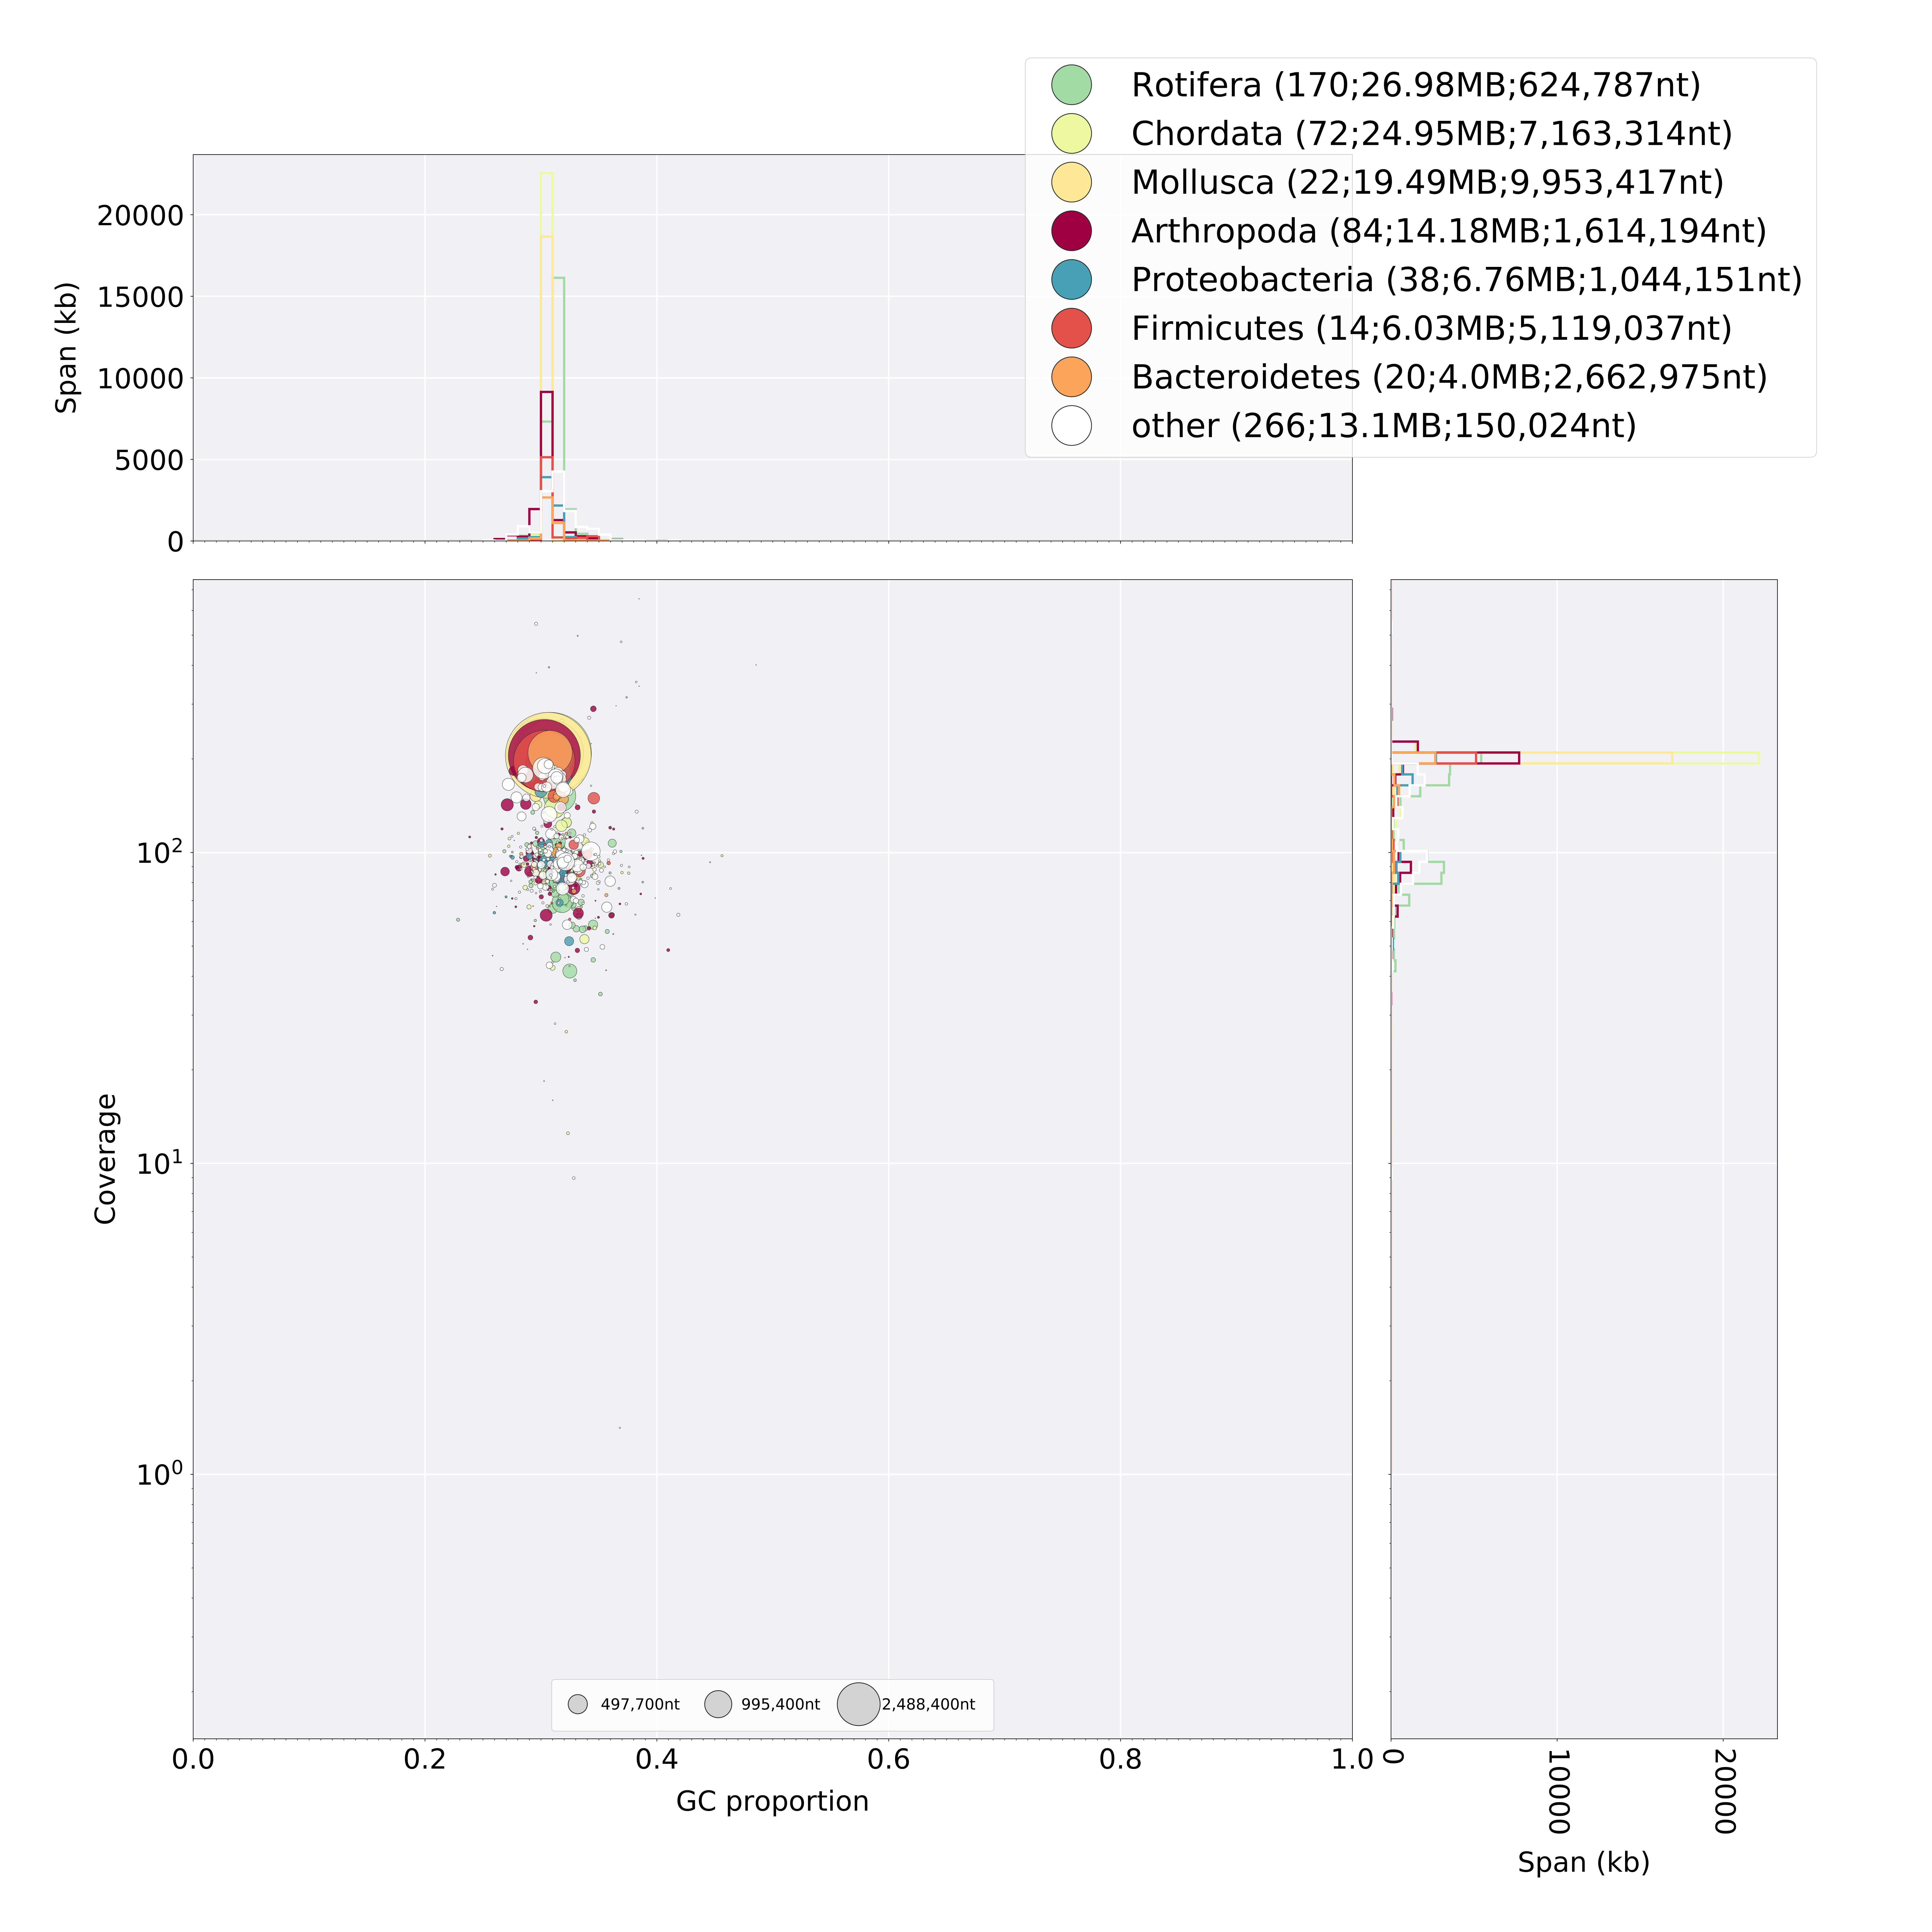
\includegraphics[width=15cm]{fig/benchmark/PB_FLYE.png}
   \caption{Blobtools v1.0 analysis of a Flye assembly of the full PacBio dataset.}
   \label{fig:blobtools_flye_pb}
 \end{figure}
 
  \begin{figure}[ht]
    \centering
     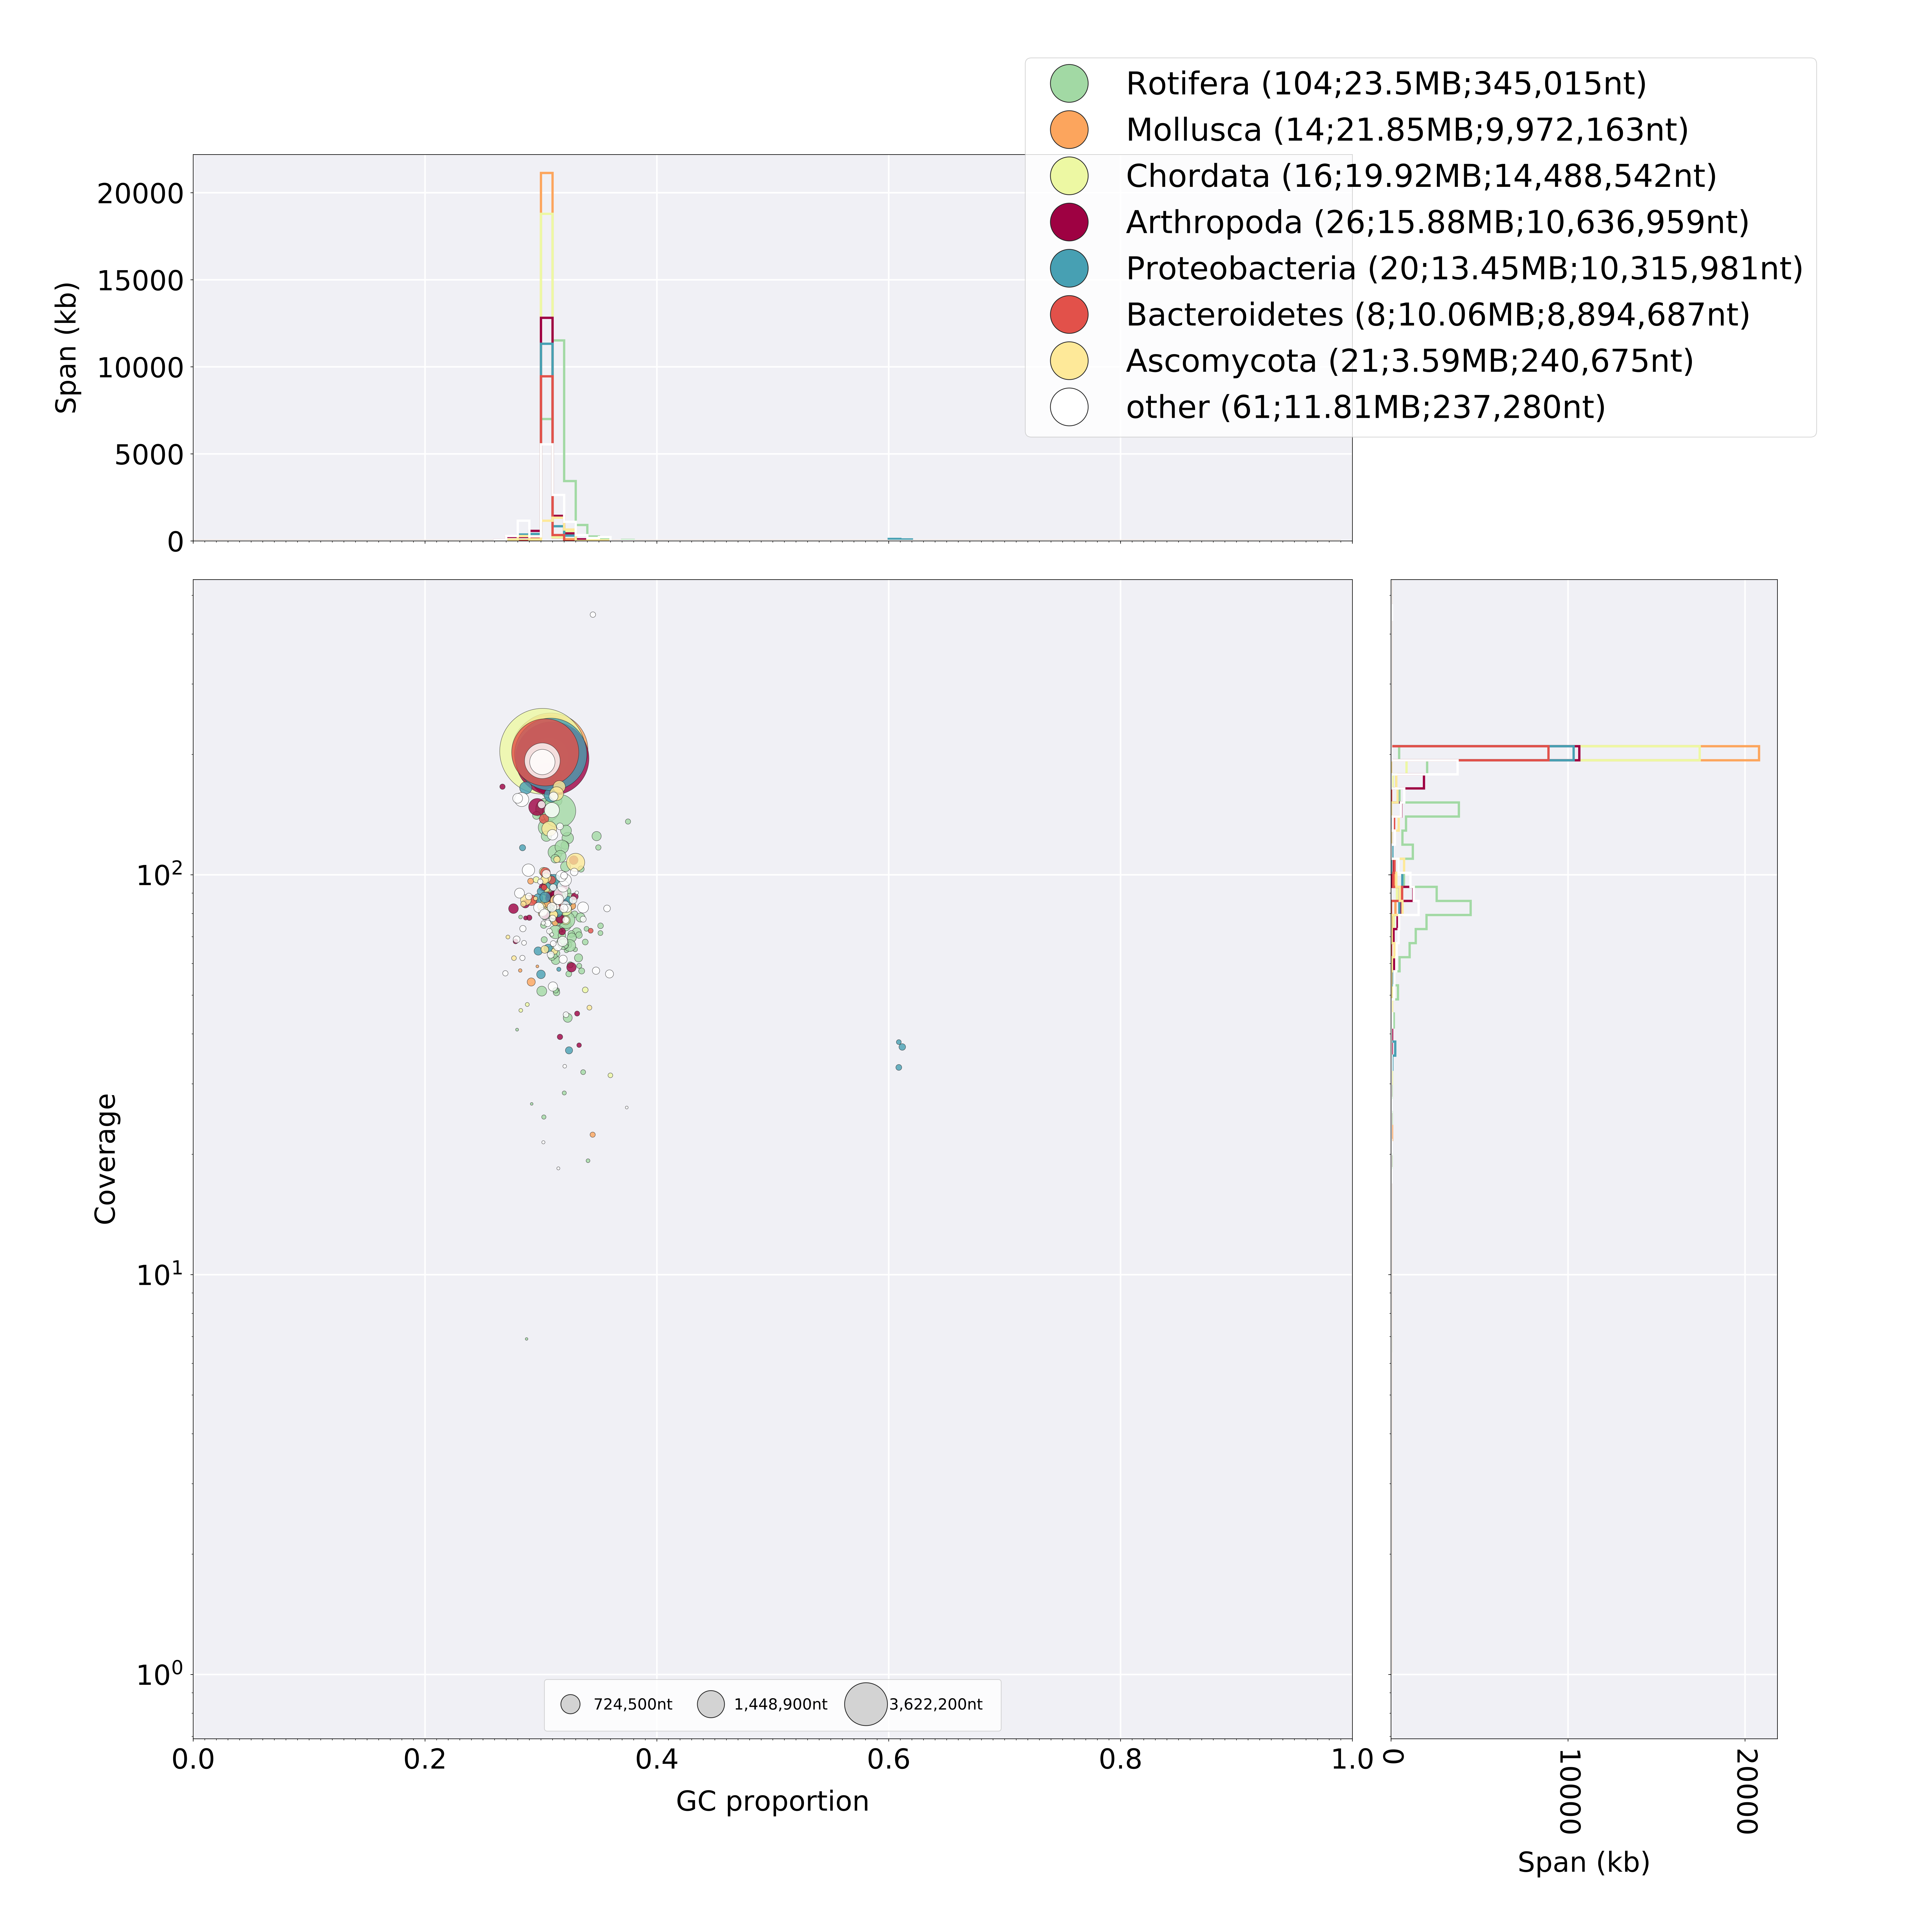
\includegraphics[width=15cm]{fig/benchmark/PB_ND.png}
   \caption{Blobtools v1.0 analysis of a NextDenovo assembly of the full PacBio dataset.}
   \label{fig:blobtools_NextDenovo_pb}
 \end{figure}

 \begin{figure}[ht]
    \centering
     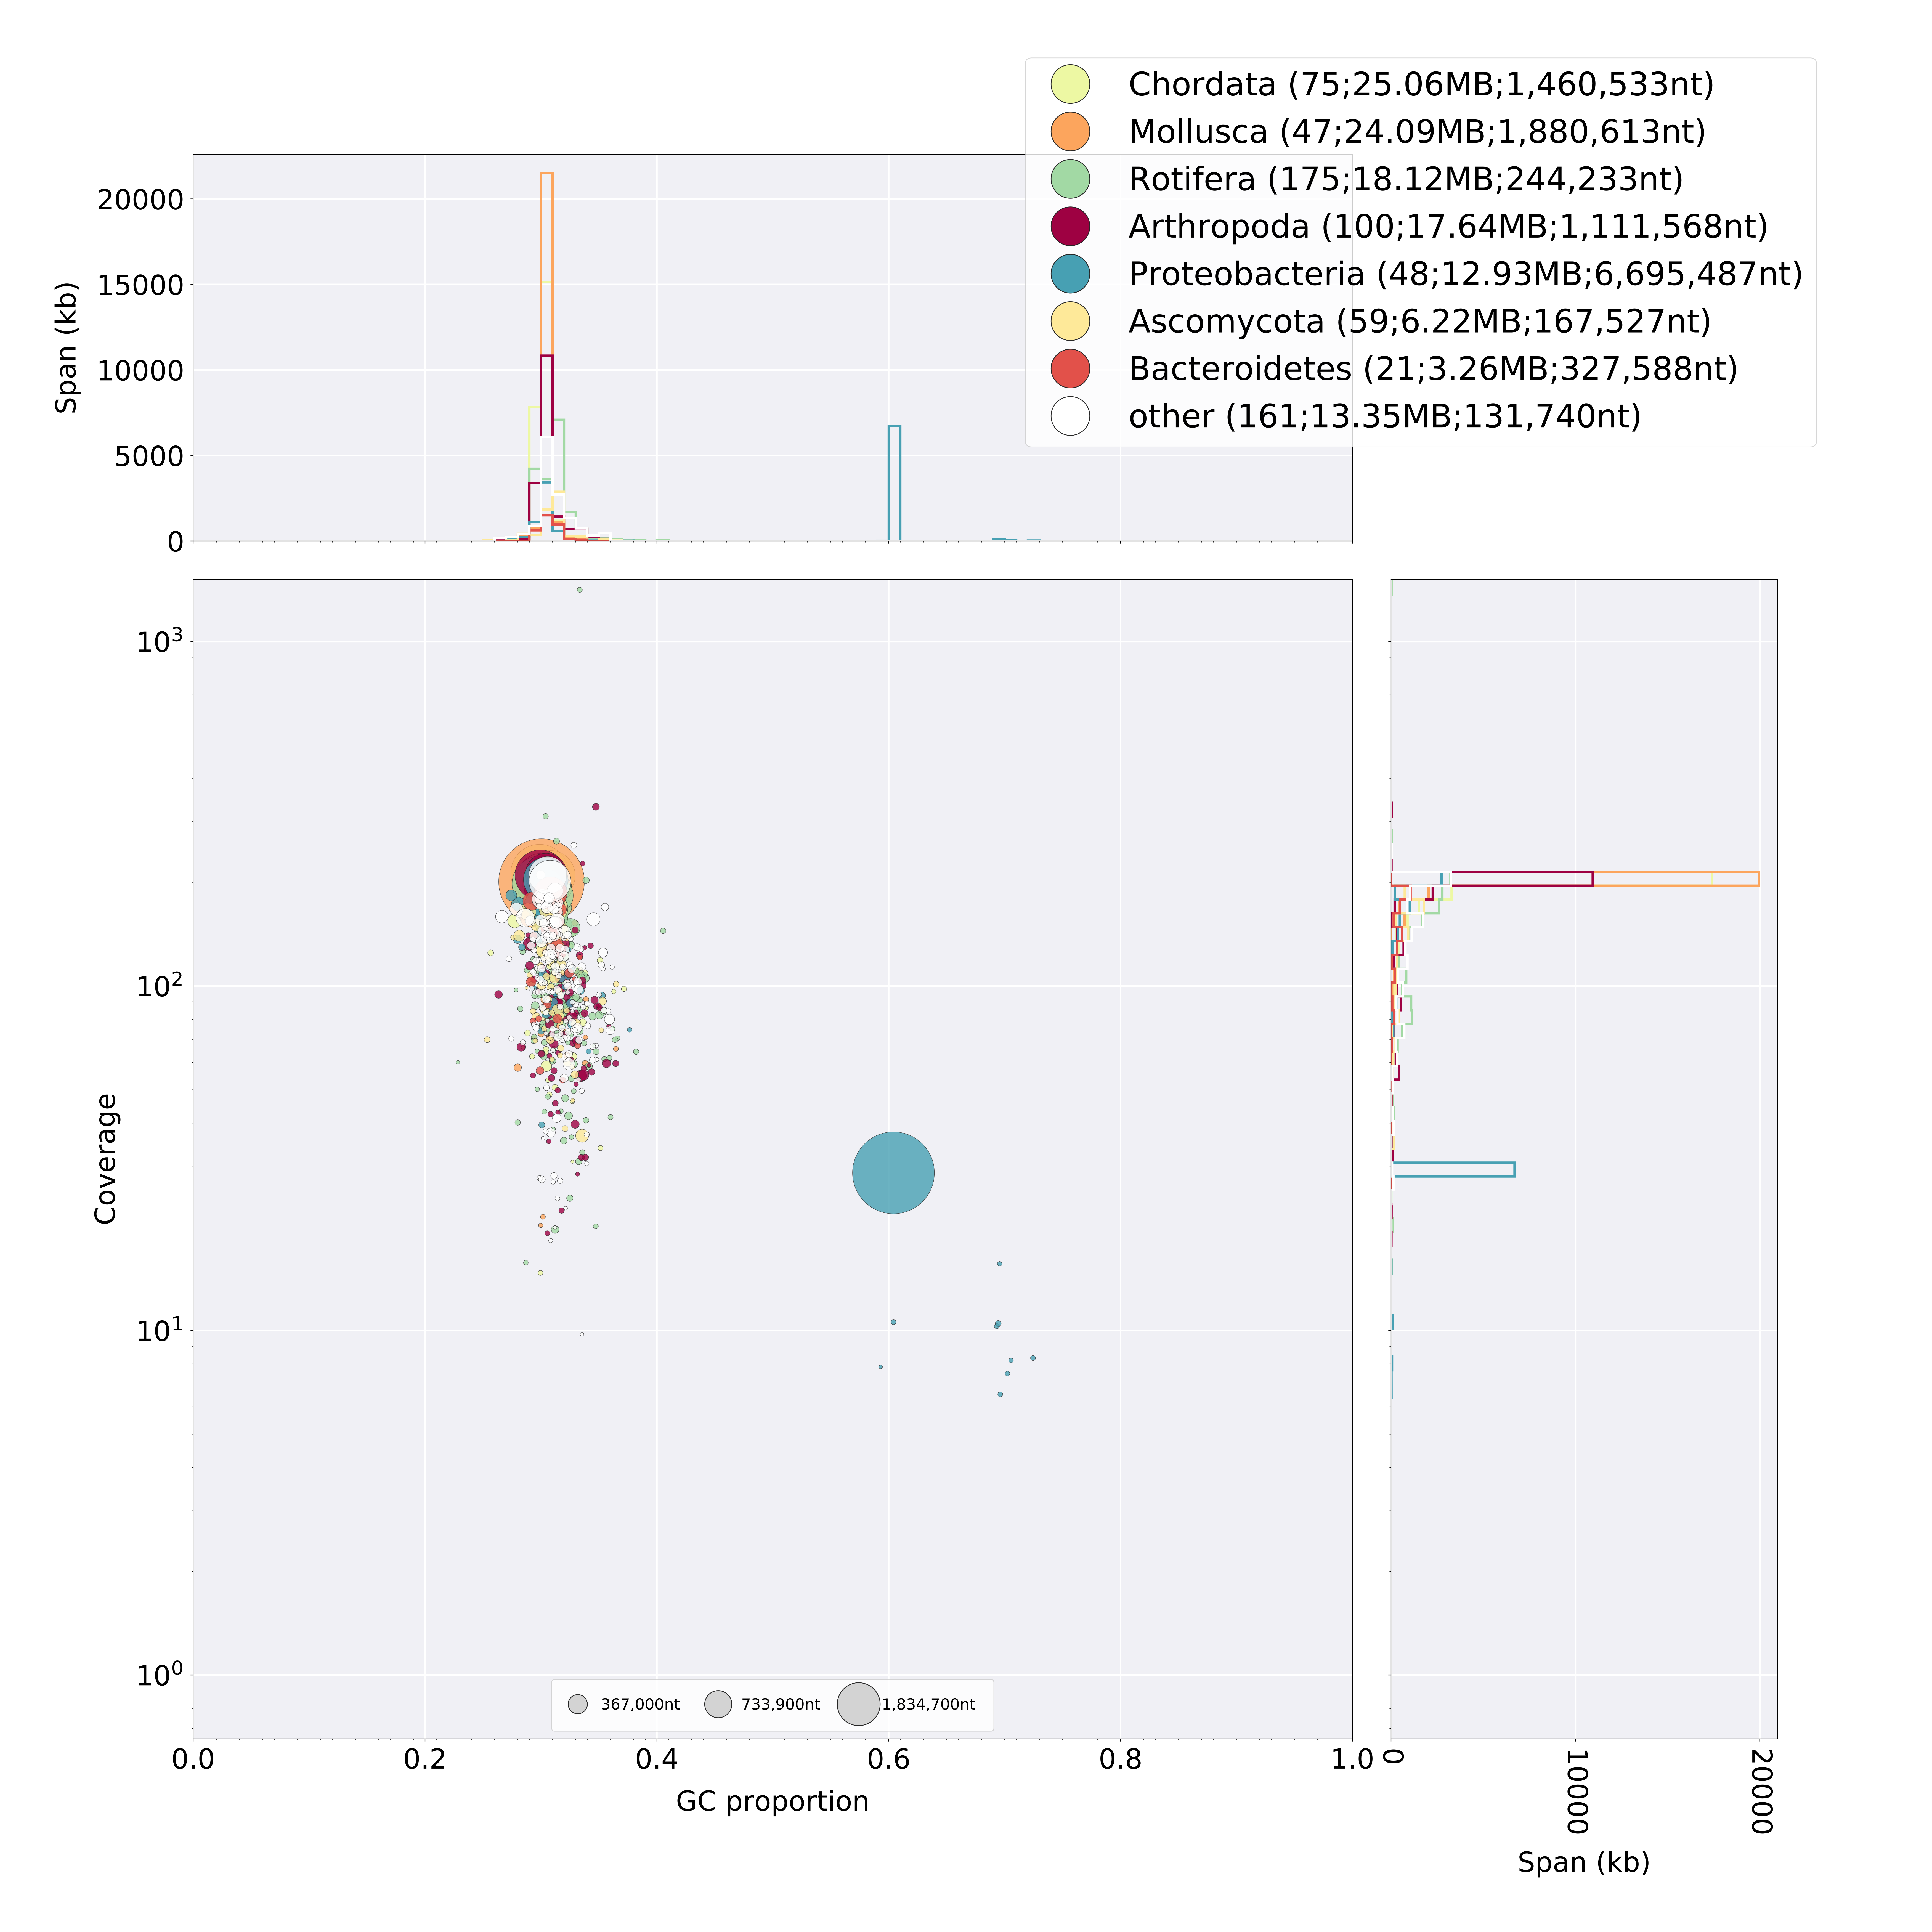
\includegraphics[width=15cm]{fig/benchmark/PB_RA.png}
   \caption{Blobtools v1.0 analysis of a Ra assembly of the full PacBio dataset.}
   \label{fig:blobtools_ra_pb}
 \end{figure}
 
  \begin{figure}[ht]
    \centering
     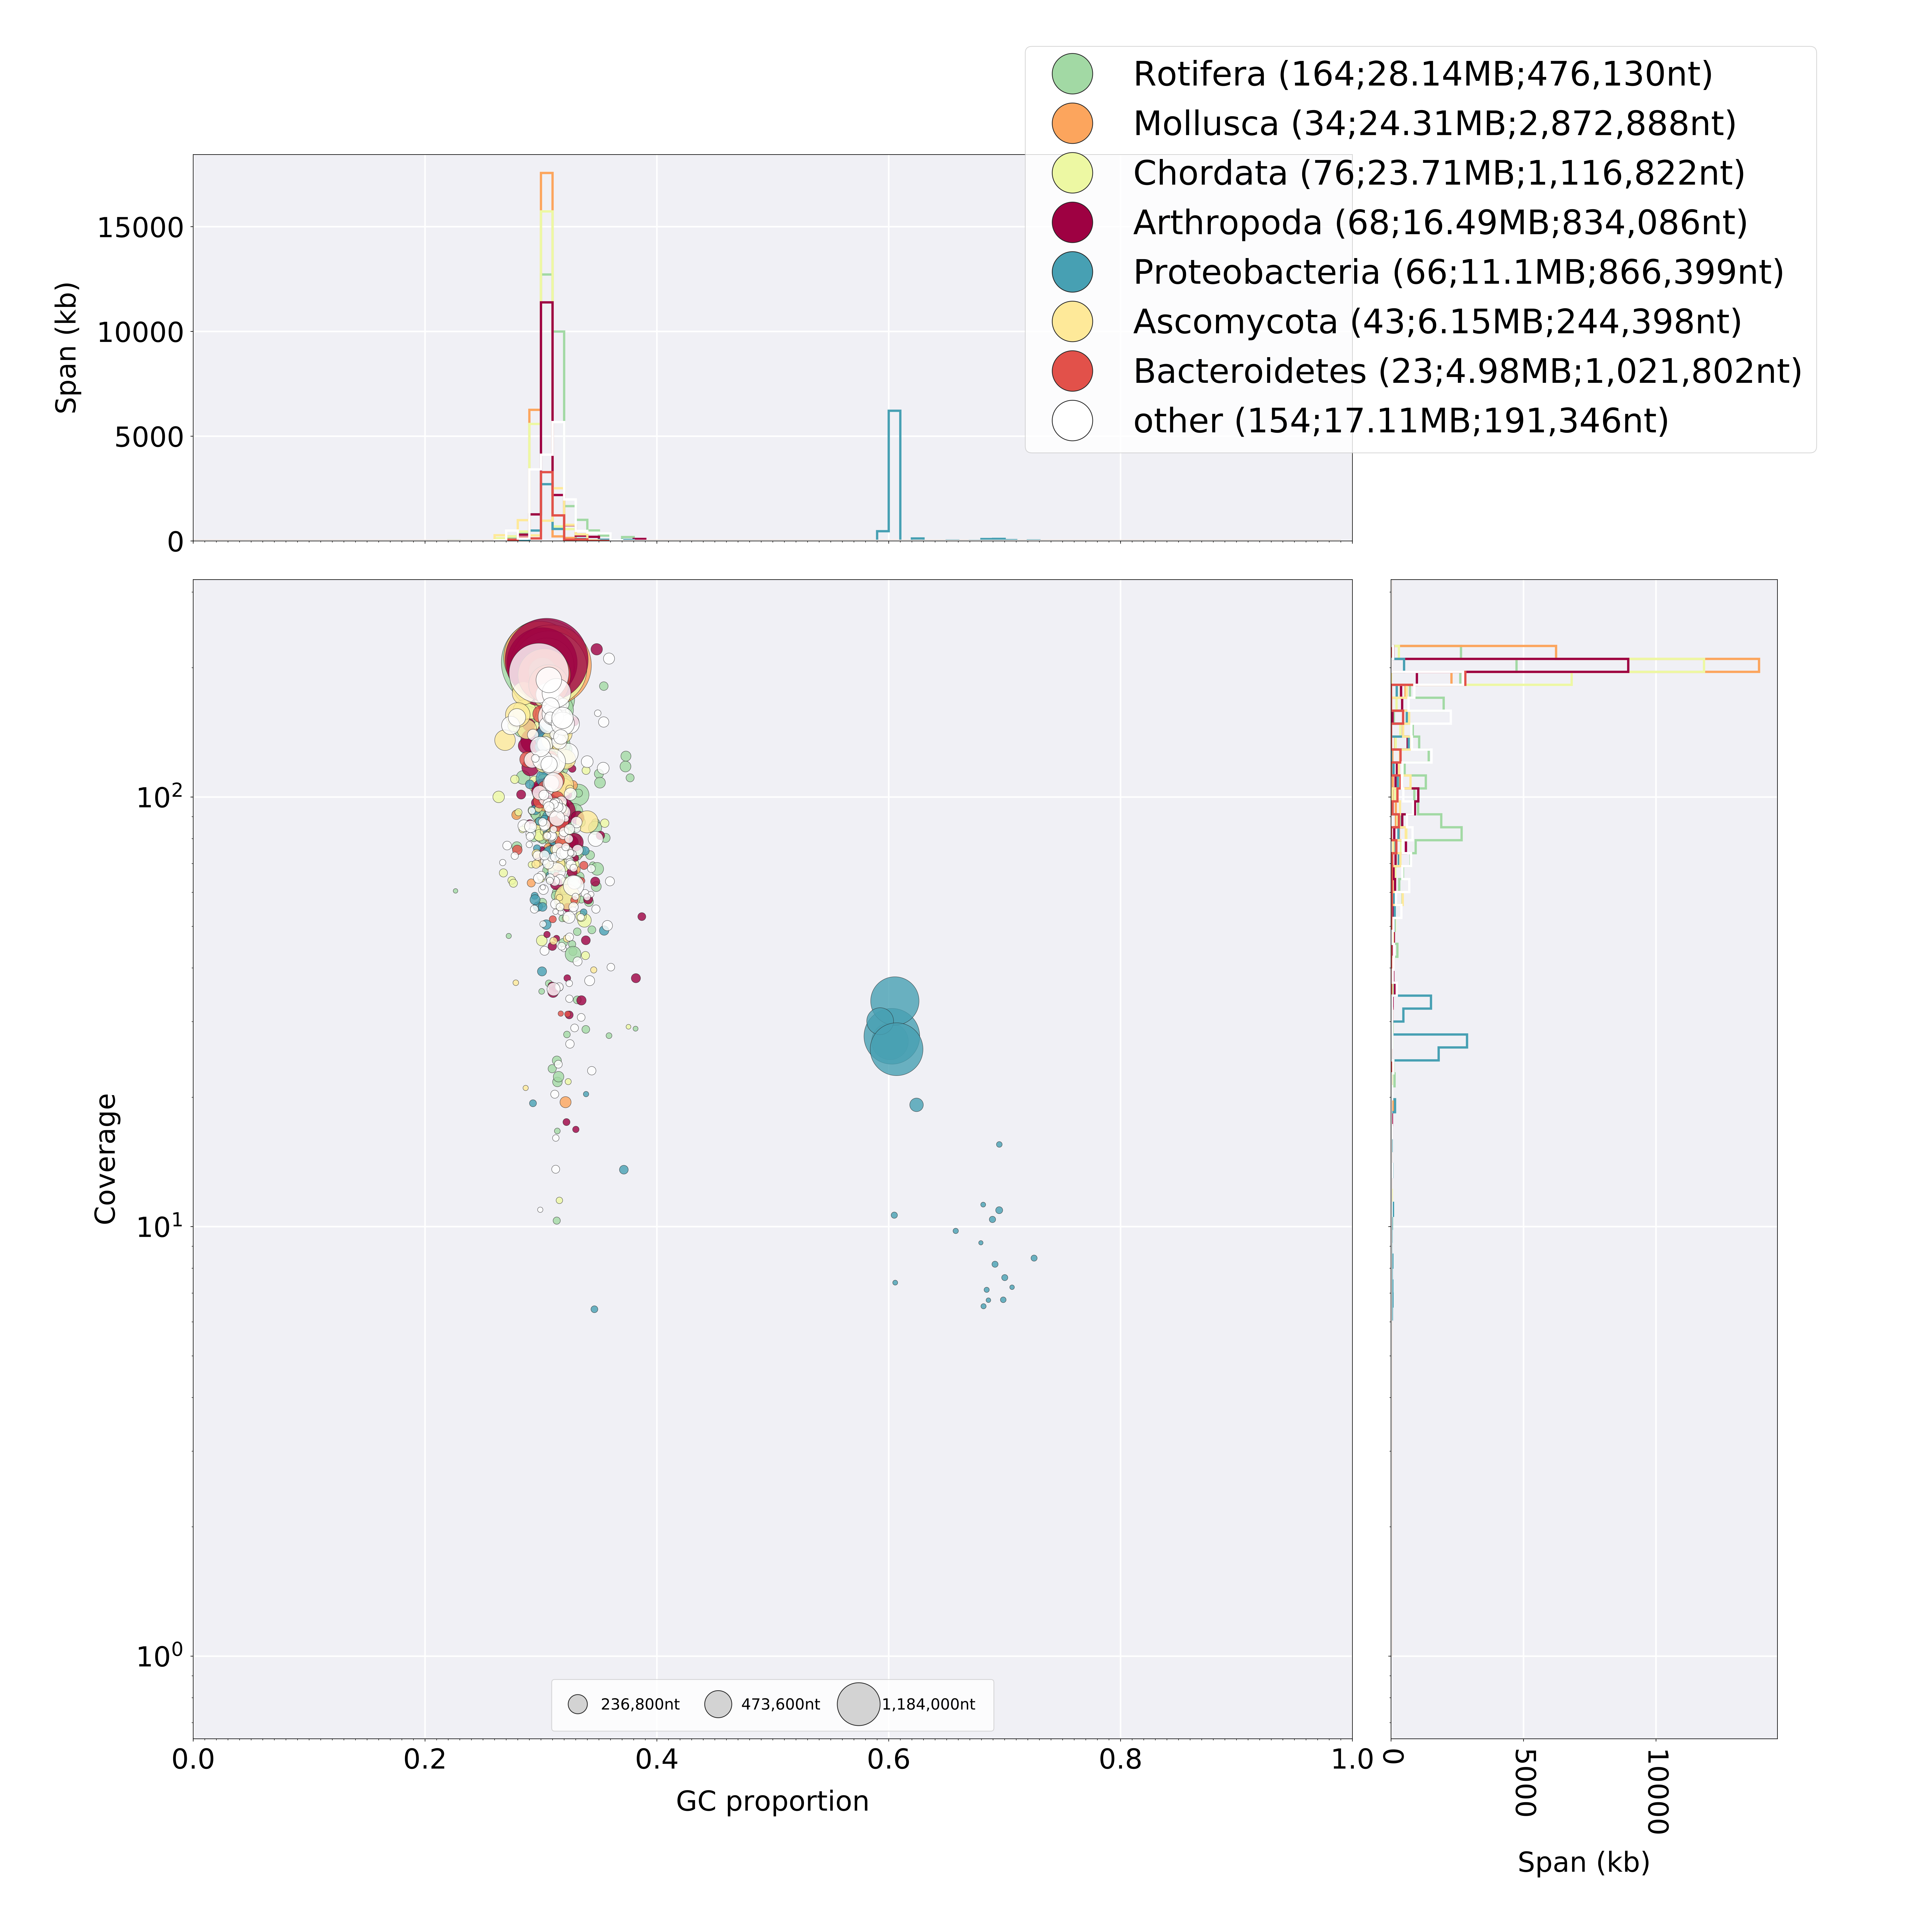
\includegraphics[width=15cm]{fig/benchmark/PB_RAVEN.png}
   \caption{Blobtools v1.0 analysis of a Raven assembly of the full PacBio dataset.}
   \label{fig:blobtools_raven_pb}
 \end{figure}
 
  \begin{figure}[ht]
    \centering
     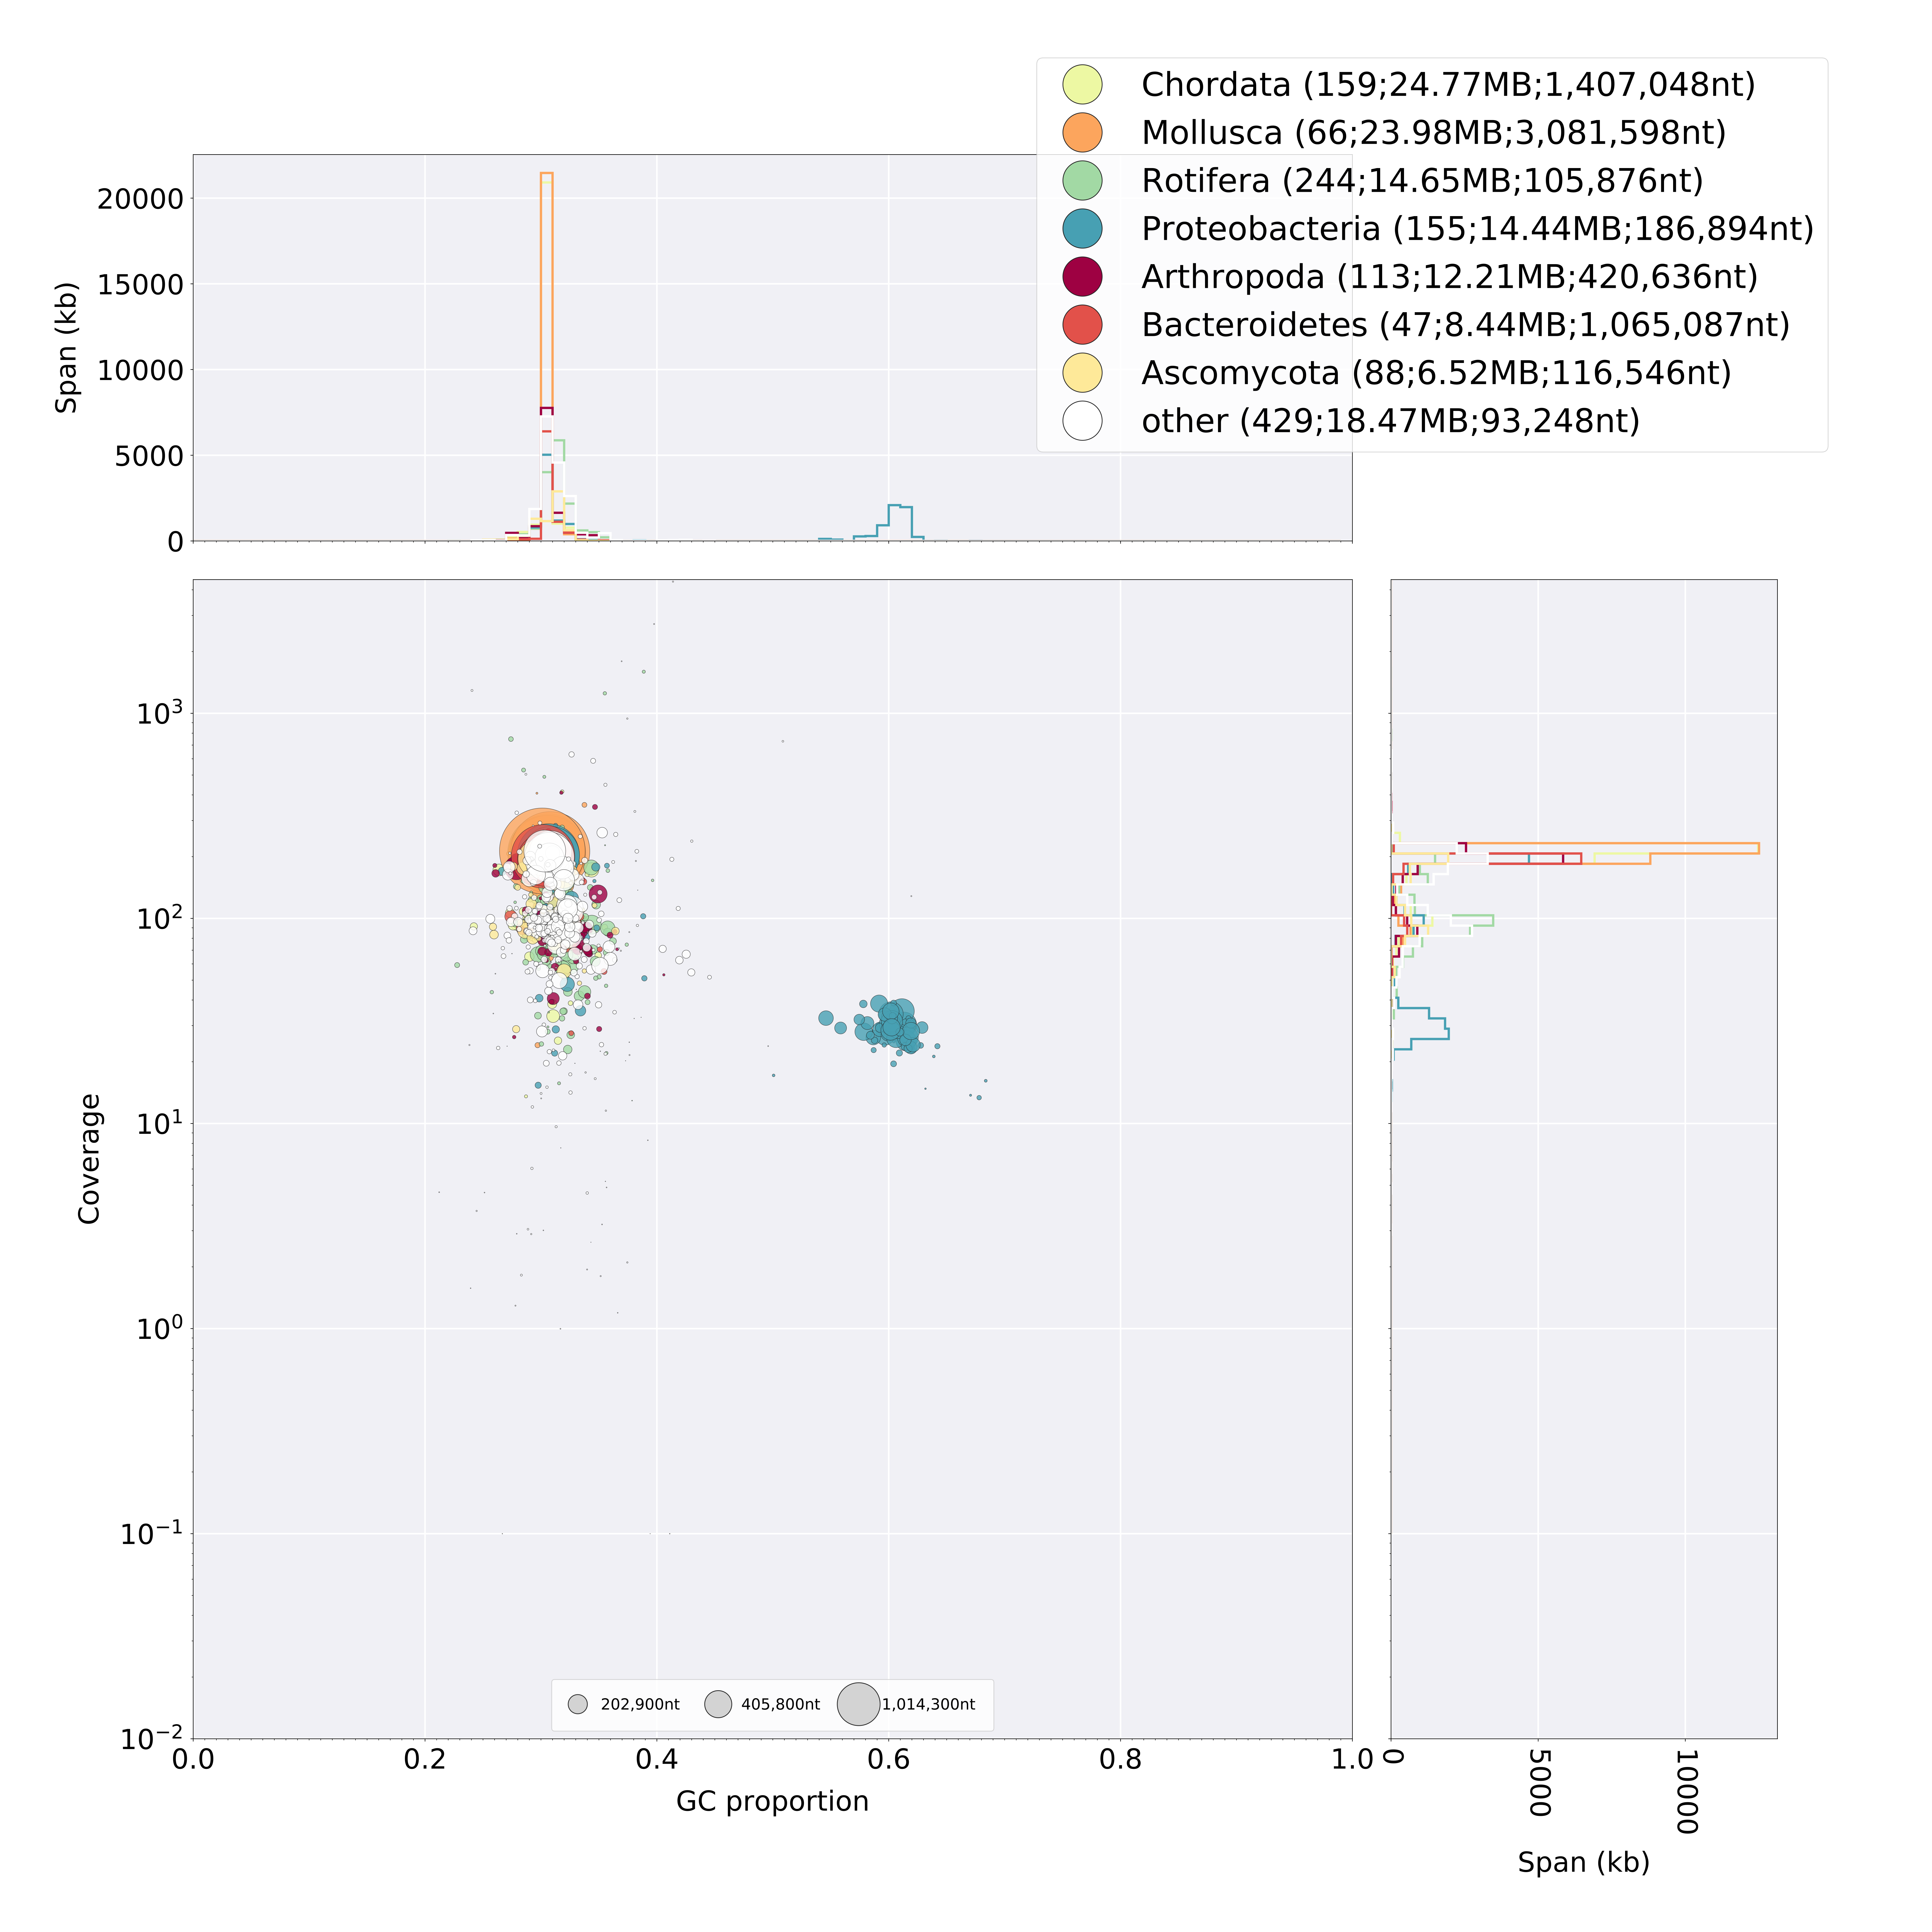
\includegraphics[width=15cm]{fig/benchmark/PB_SHASTA.png}
   \caption{Blobtools v1.0 analysis of a Shasta assembly of the full PacBio dataset.}
   \label{fig:blobtools_shasta_pb}
 \end{figure}

 \begin{figure}[ht]
    \centering
     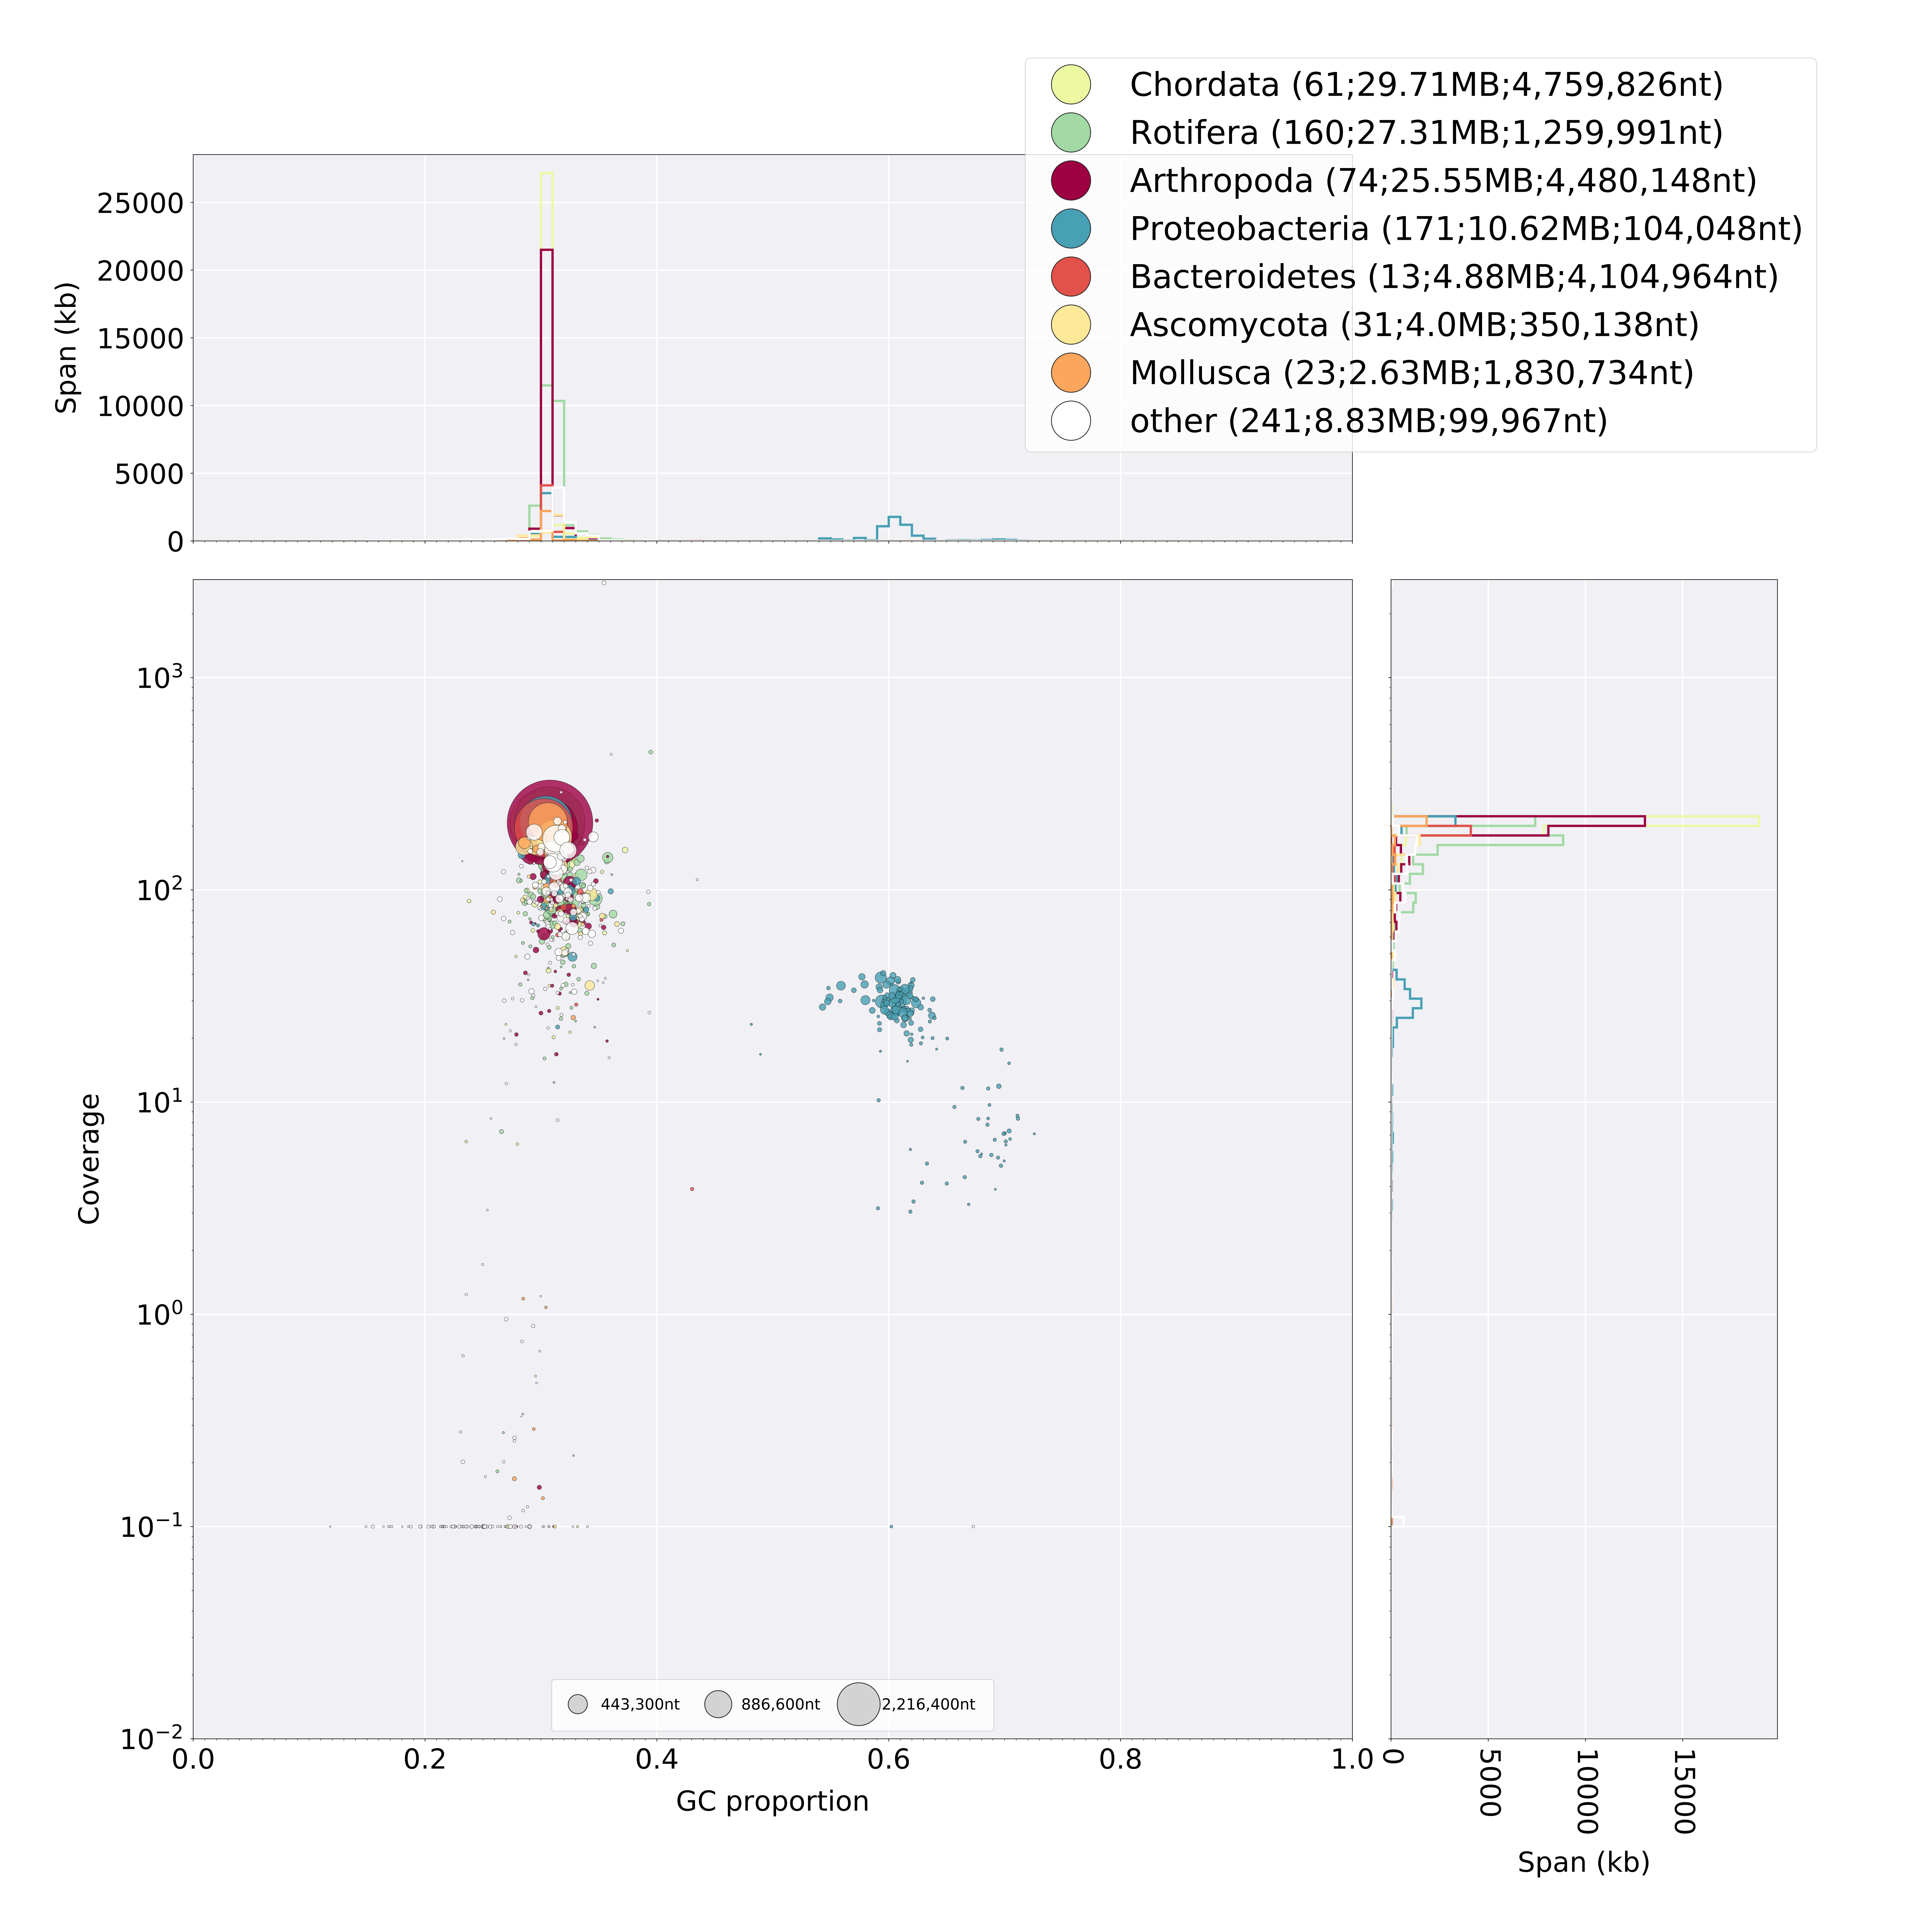
\includegraphics[width=15cm]{fig/benchmark/PB_WTDBG.png}
   \caption{Blobtools v1.0 analysis of a wtdbg2 assembly of the full PacBio dataset.}
   \label{fig:blobtools_wtdbg2_pb}
 \end{figure}

    \begin{figure}[ht]
    \centering
     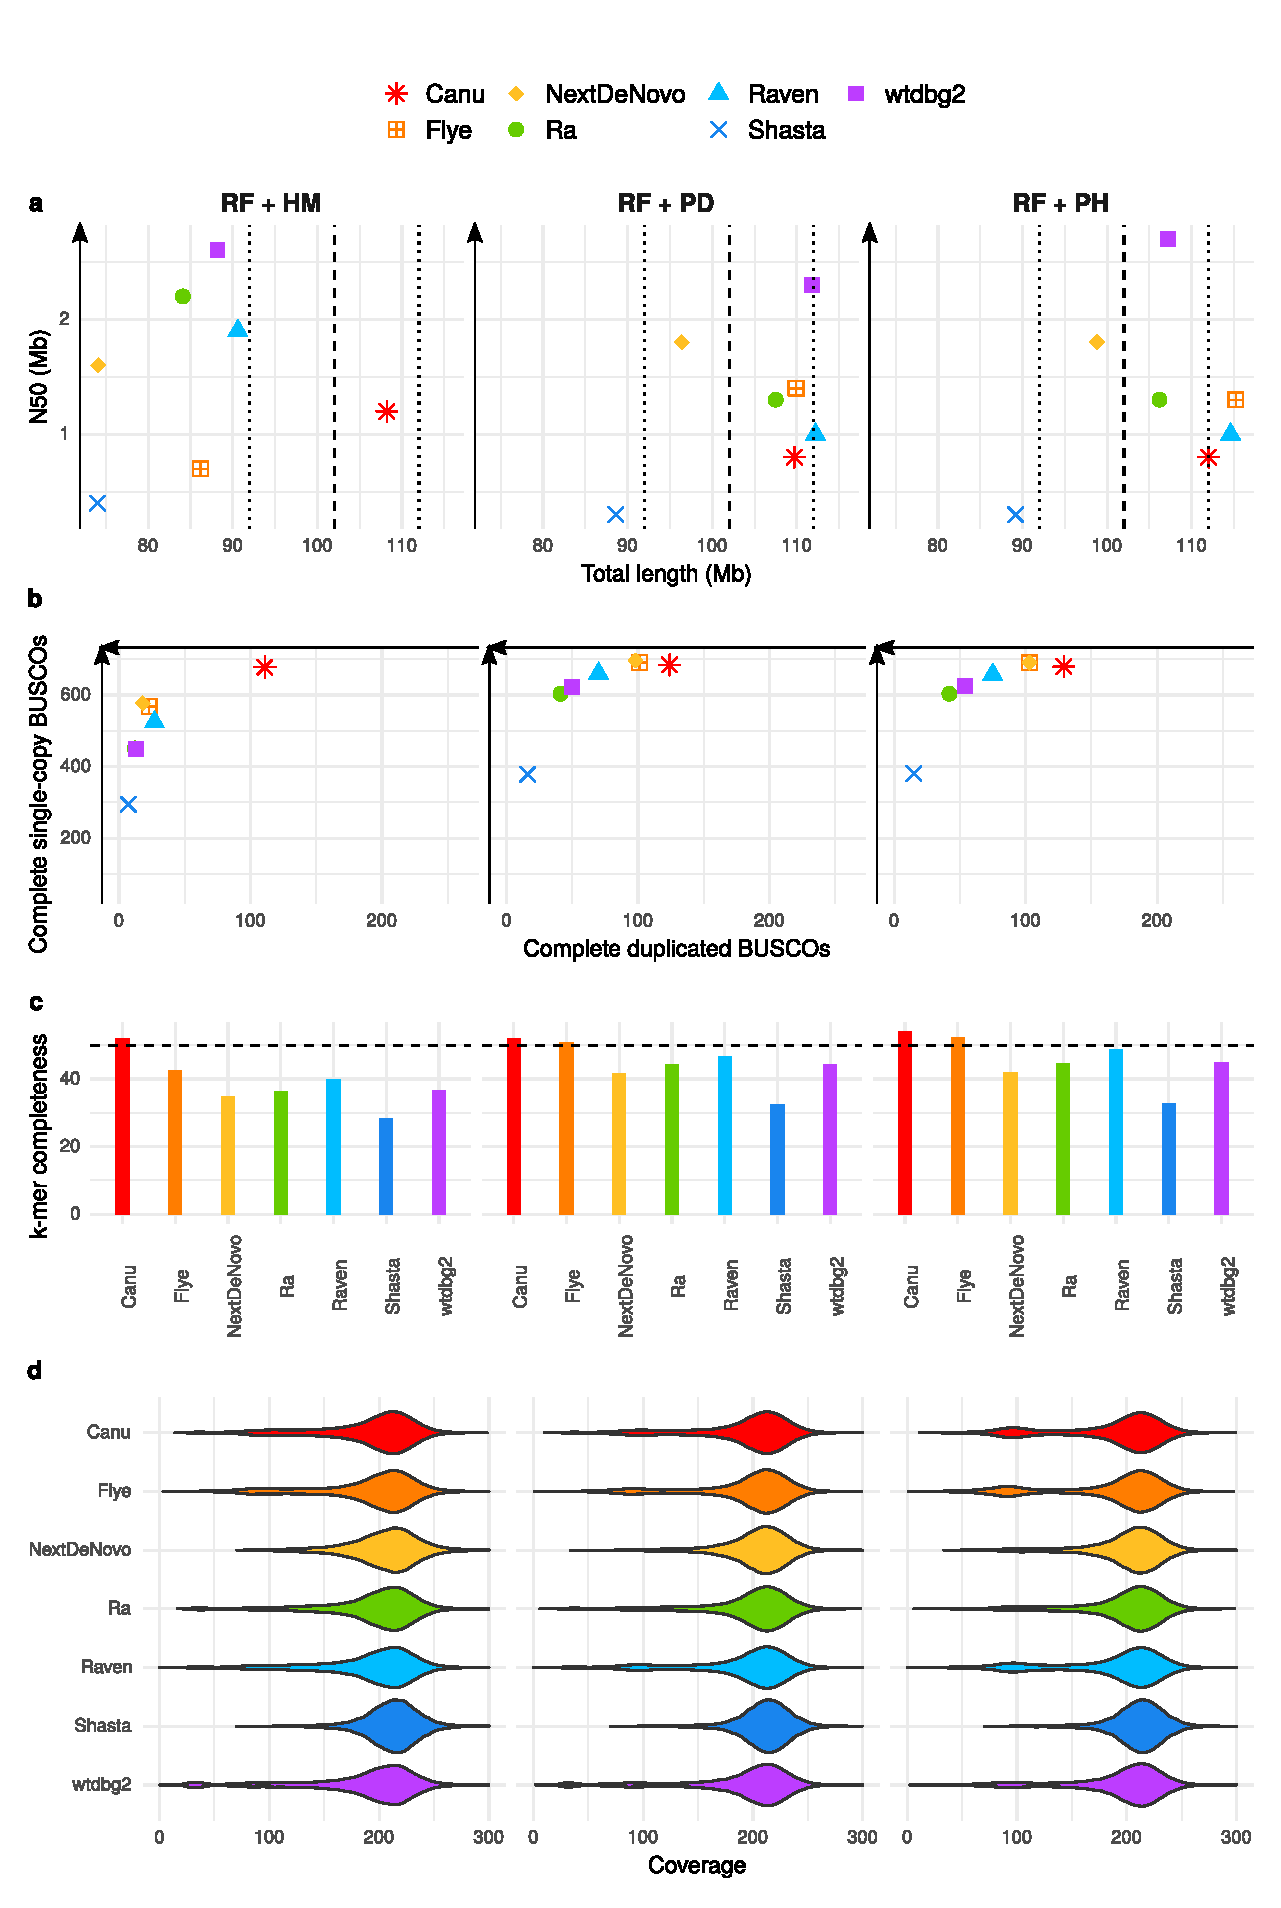
\includegraphics[width=13.5cm]{fig/benchmark/supp_pacbio_filtering_purging_v20201012.eps}
   \caption{Statistics of PacBio assemblies obtained from the filtered PacBio dataset of reads longer than 15 kb, with a subsequent removal of uncollapsed haplotypes with HaploMerger2 (HM), purge\_dups (PD), or purge\_haplotigs (PH). a) N50 plotted against total assembly length. The dashed line indicates the expected genome size, with a +/- 10 Mb margin delimited by the dotted lines. b) Number of complete single-copy BUSCOs plotted against number of complete duplicated BUSCOs, from a total of 954 orthologs. c) \textit{k}-mer completeness. The dashed line indicates the expected 50\% completeness. d) Long-read coverage distribution over the contigs.}
   \label{fig:pacbio_filtering_purging}
 \end{figure}
 
     \begin{figure}[ht]
    \centering
     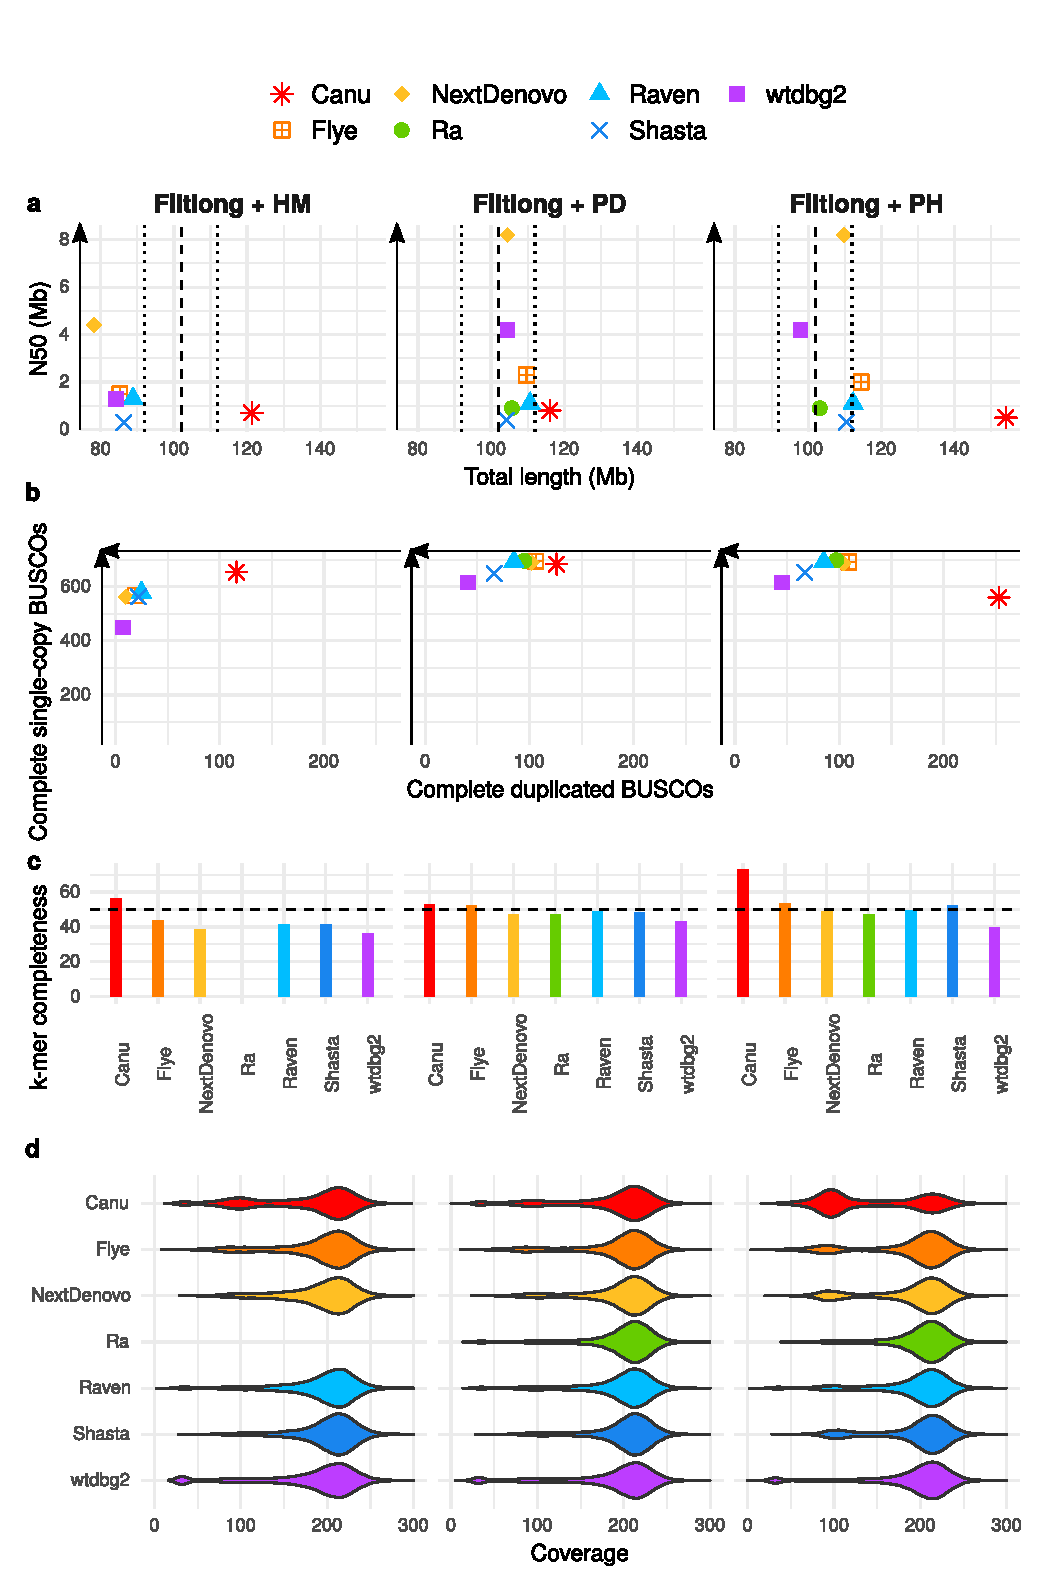
\includegraphics[width=13.5cm]{fig/benchmark/supp_pacbio_filtlong_purging.eps}
   \caption{Statistics of PacBio assemblies obtained from the PacBio dataset filtered with Filtlong, with a subsequent removal of uncollapsed haplotypes with HaploMerger2 (HM), purge\_dups (PD), or purge\_haplotigs (PH). a) N50 plotted against total assembly length. The dashed line indicates the expected genome size, with a +/- 10 Mb margin delimited by the dotted lines. b) Number of complete single-copy BUSCOs plotted against number of complete duplicated BUSCOs, from a total of 954 orthologs. c) \textit{k}-mer completeness. The dashed line indicates the expected 50\% completeness. d) Long-read coverage distribution over the contigs.}
   \label{fig:pacbio_filtlong_purging}
 \end{figure}
 
   \begin{figure}[ht]
    \centering
     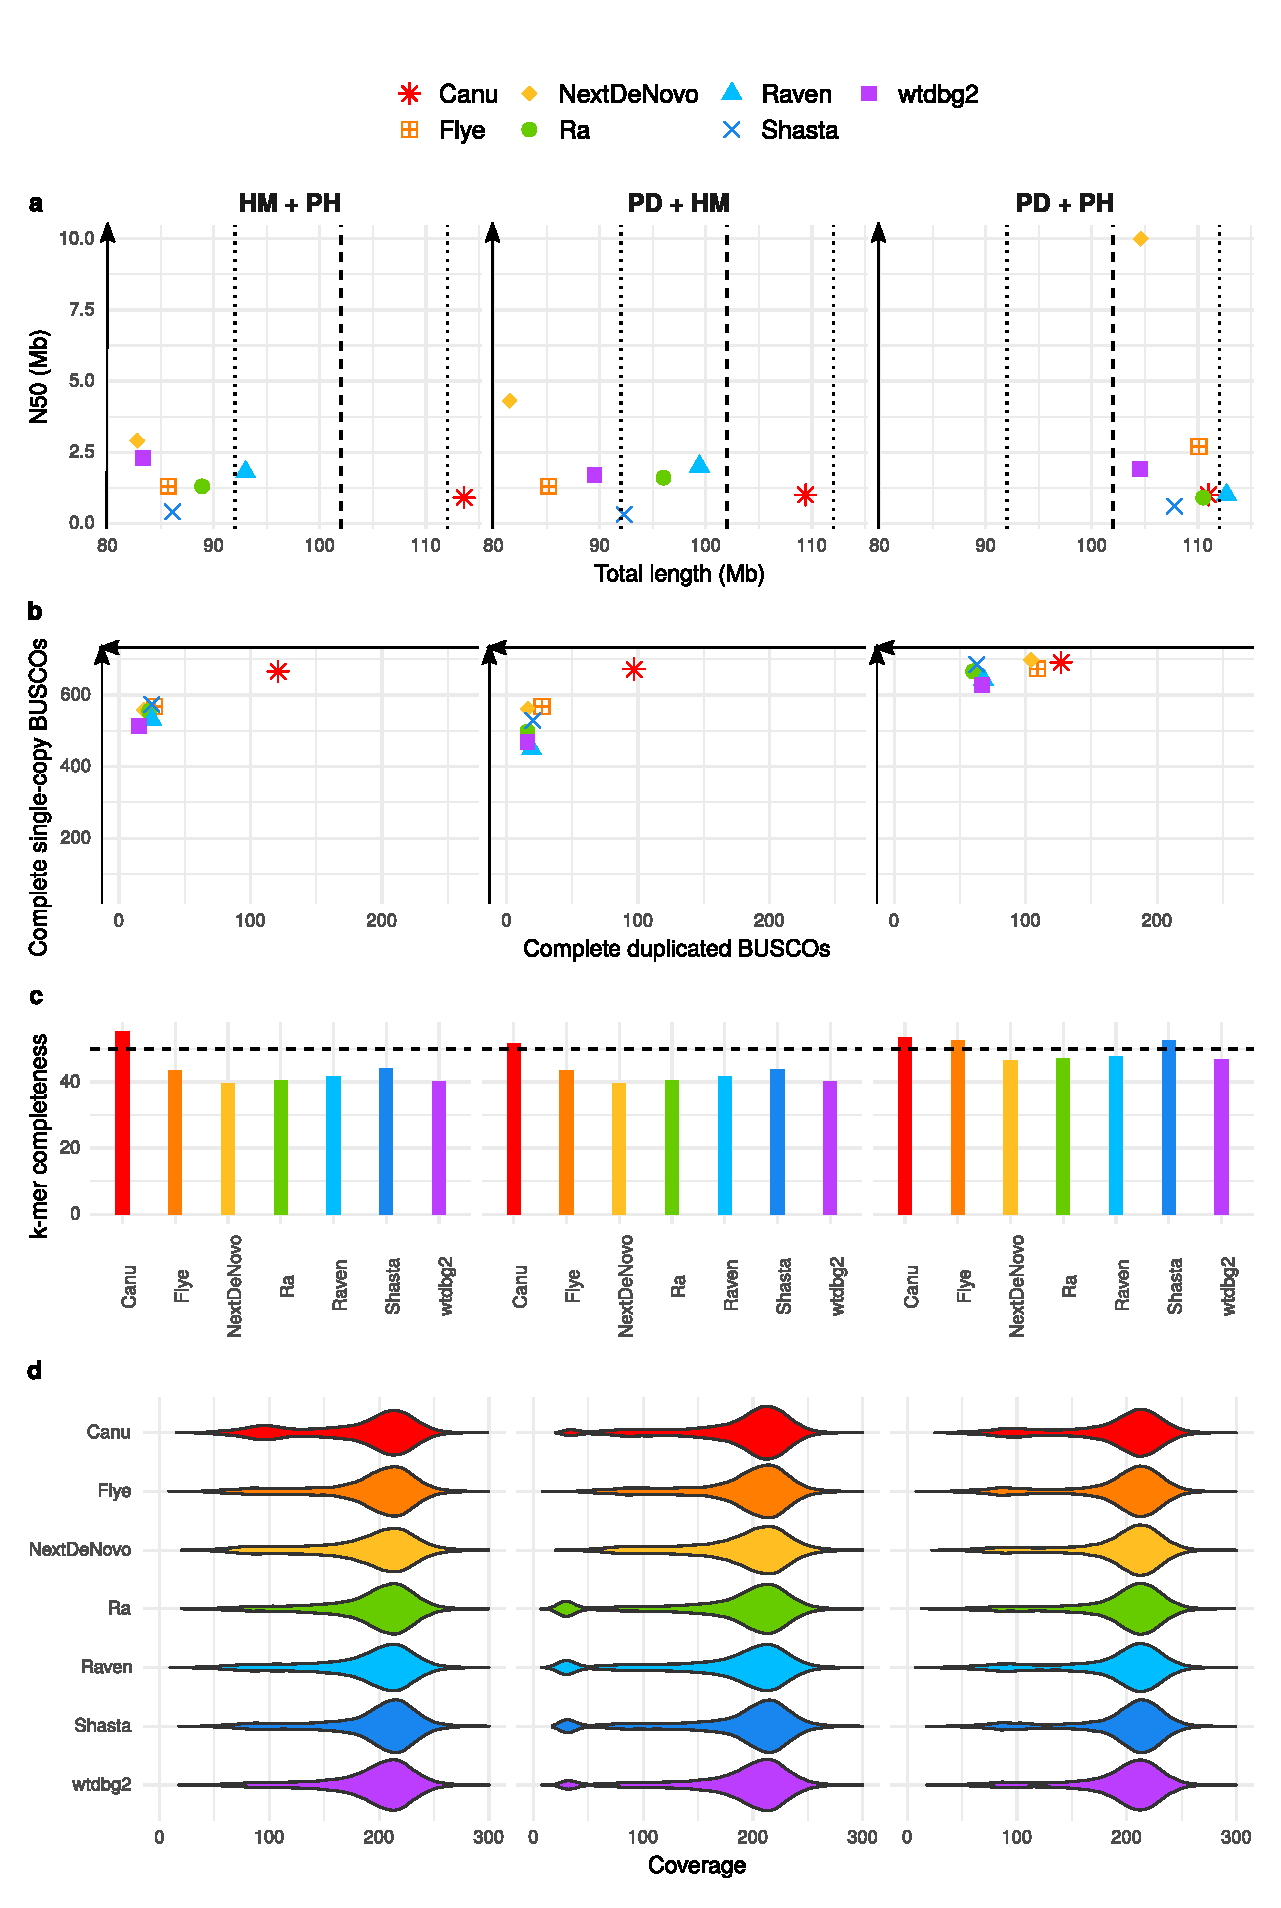
\includegraphics[width=13.5cm]{fig/benchmark/supp_pacbio_purging_combinations_v20200919.eps}
   \caption{Statistics of PacBio assemblies obtained from the full PacBio dataset with a subsequent removal of uncollapsed haplotypes with combinations of HaploMerger2 (HM), purge\_dups (PD), and purge\_haplotigs (PH). a) N50 plotted against total assembly length. The dashed line indicates the expected genome size, with a +/- 10 Mb margin delimited by the dotted lines. b) Number of complete single-copy BUSCOs plotted against number of complete duplicated BUSCOs, from a total of 954 orthologs. c) \textit{k}-mer completeness. The dashed line indicates the expected 50\% completeness. d) Long-read coverage distribution over the contigs.}
   \label{fig:pacbio_purging_combinations}
 \end{figure}
 
 
 \begin{figure}[ht]
    \centering
     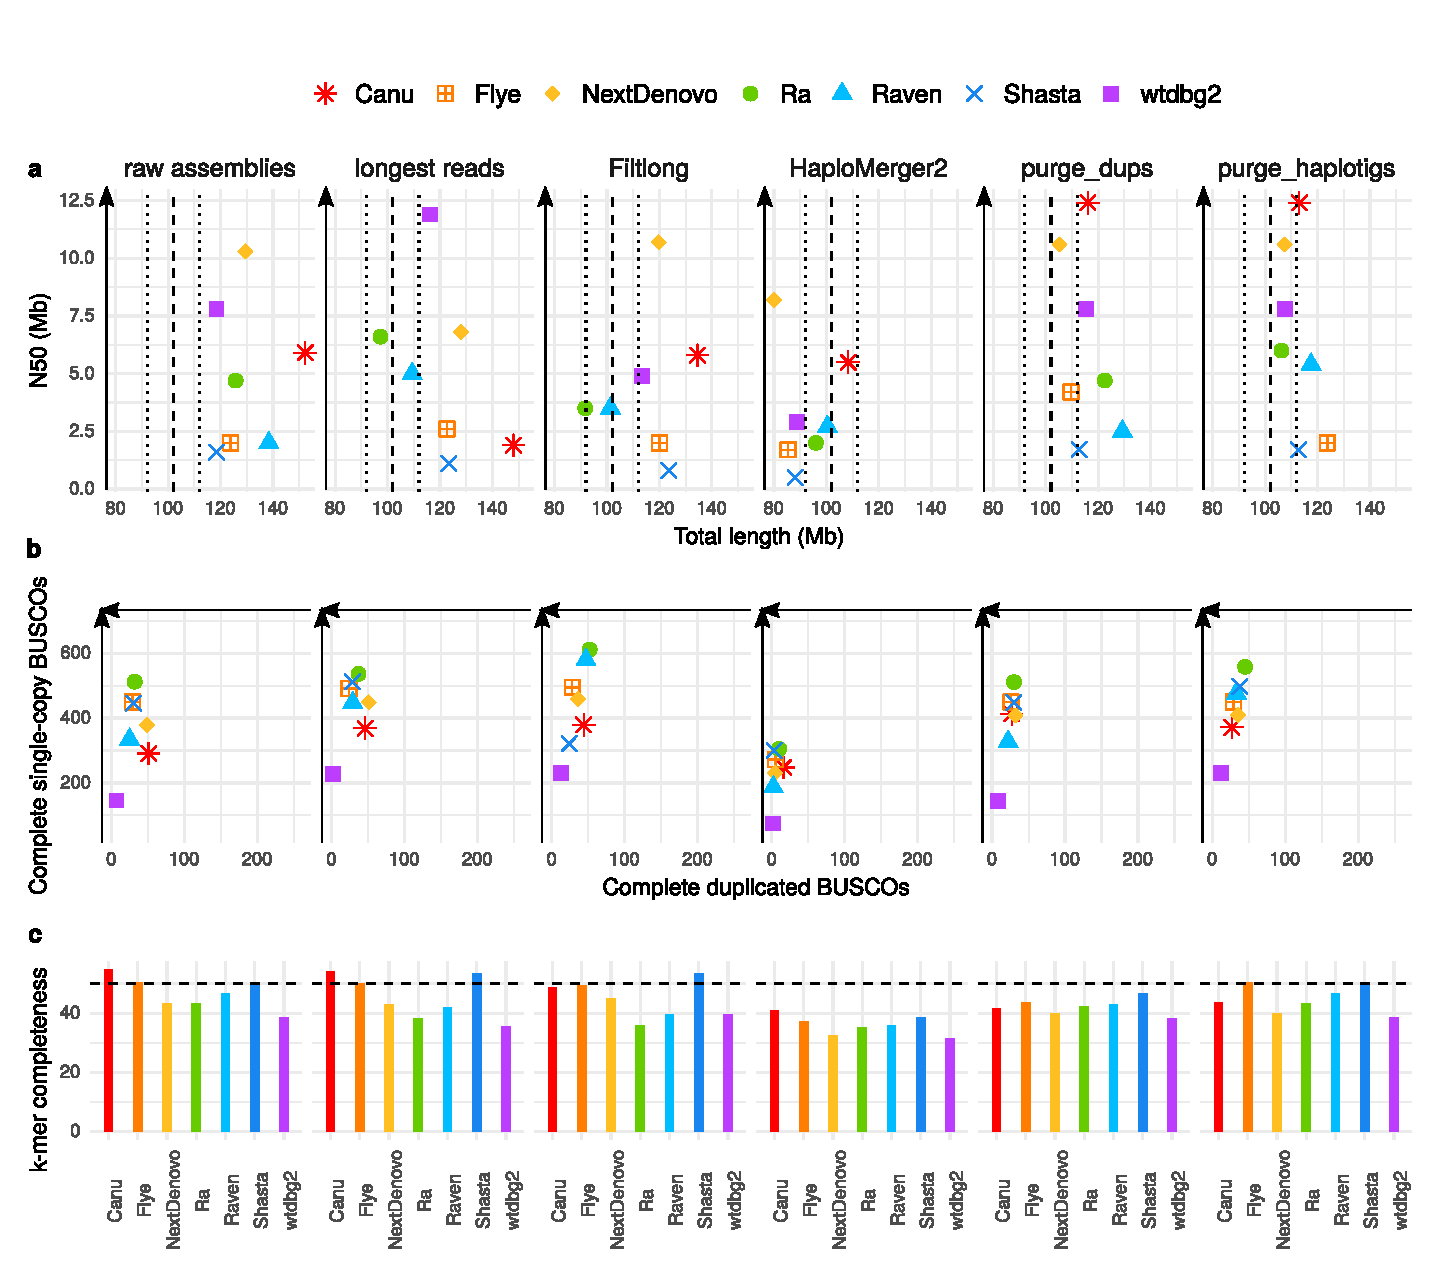
\includegraphics[width=13.5cm]{fig/benchmark/nanopore_all_v20210317.eps}
   \caption{Statistics of raw assemblies obtained from the full Nanopore dataset (raw assemblies), with a preliminary read filtering step (keeping only reads larger than 30 kb, or those selected by Filtlong based on quality and length) or a subsequent removal of uncollapsed haplotypes with HaploMerger2, purge\_dups, or purge\_haplotigs. a) N50 plotted against total assembly length. The dashed line indicates the expected genome size, with +/- 10 Mb margin delimited by the dotted lines. b) Number of complete single-copy BUSCOs plotted against number of complete duplicated BUSCOs, from a total of 954 orthologs. c) \textit{k}-mer completeness. The dashed line indicates the expected 50\% completeness.}
   \label{fig:nanopore_full_stats}
 \end{figure}
 
   \begin{figure}[ht]
    \centering
     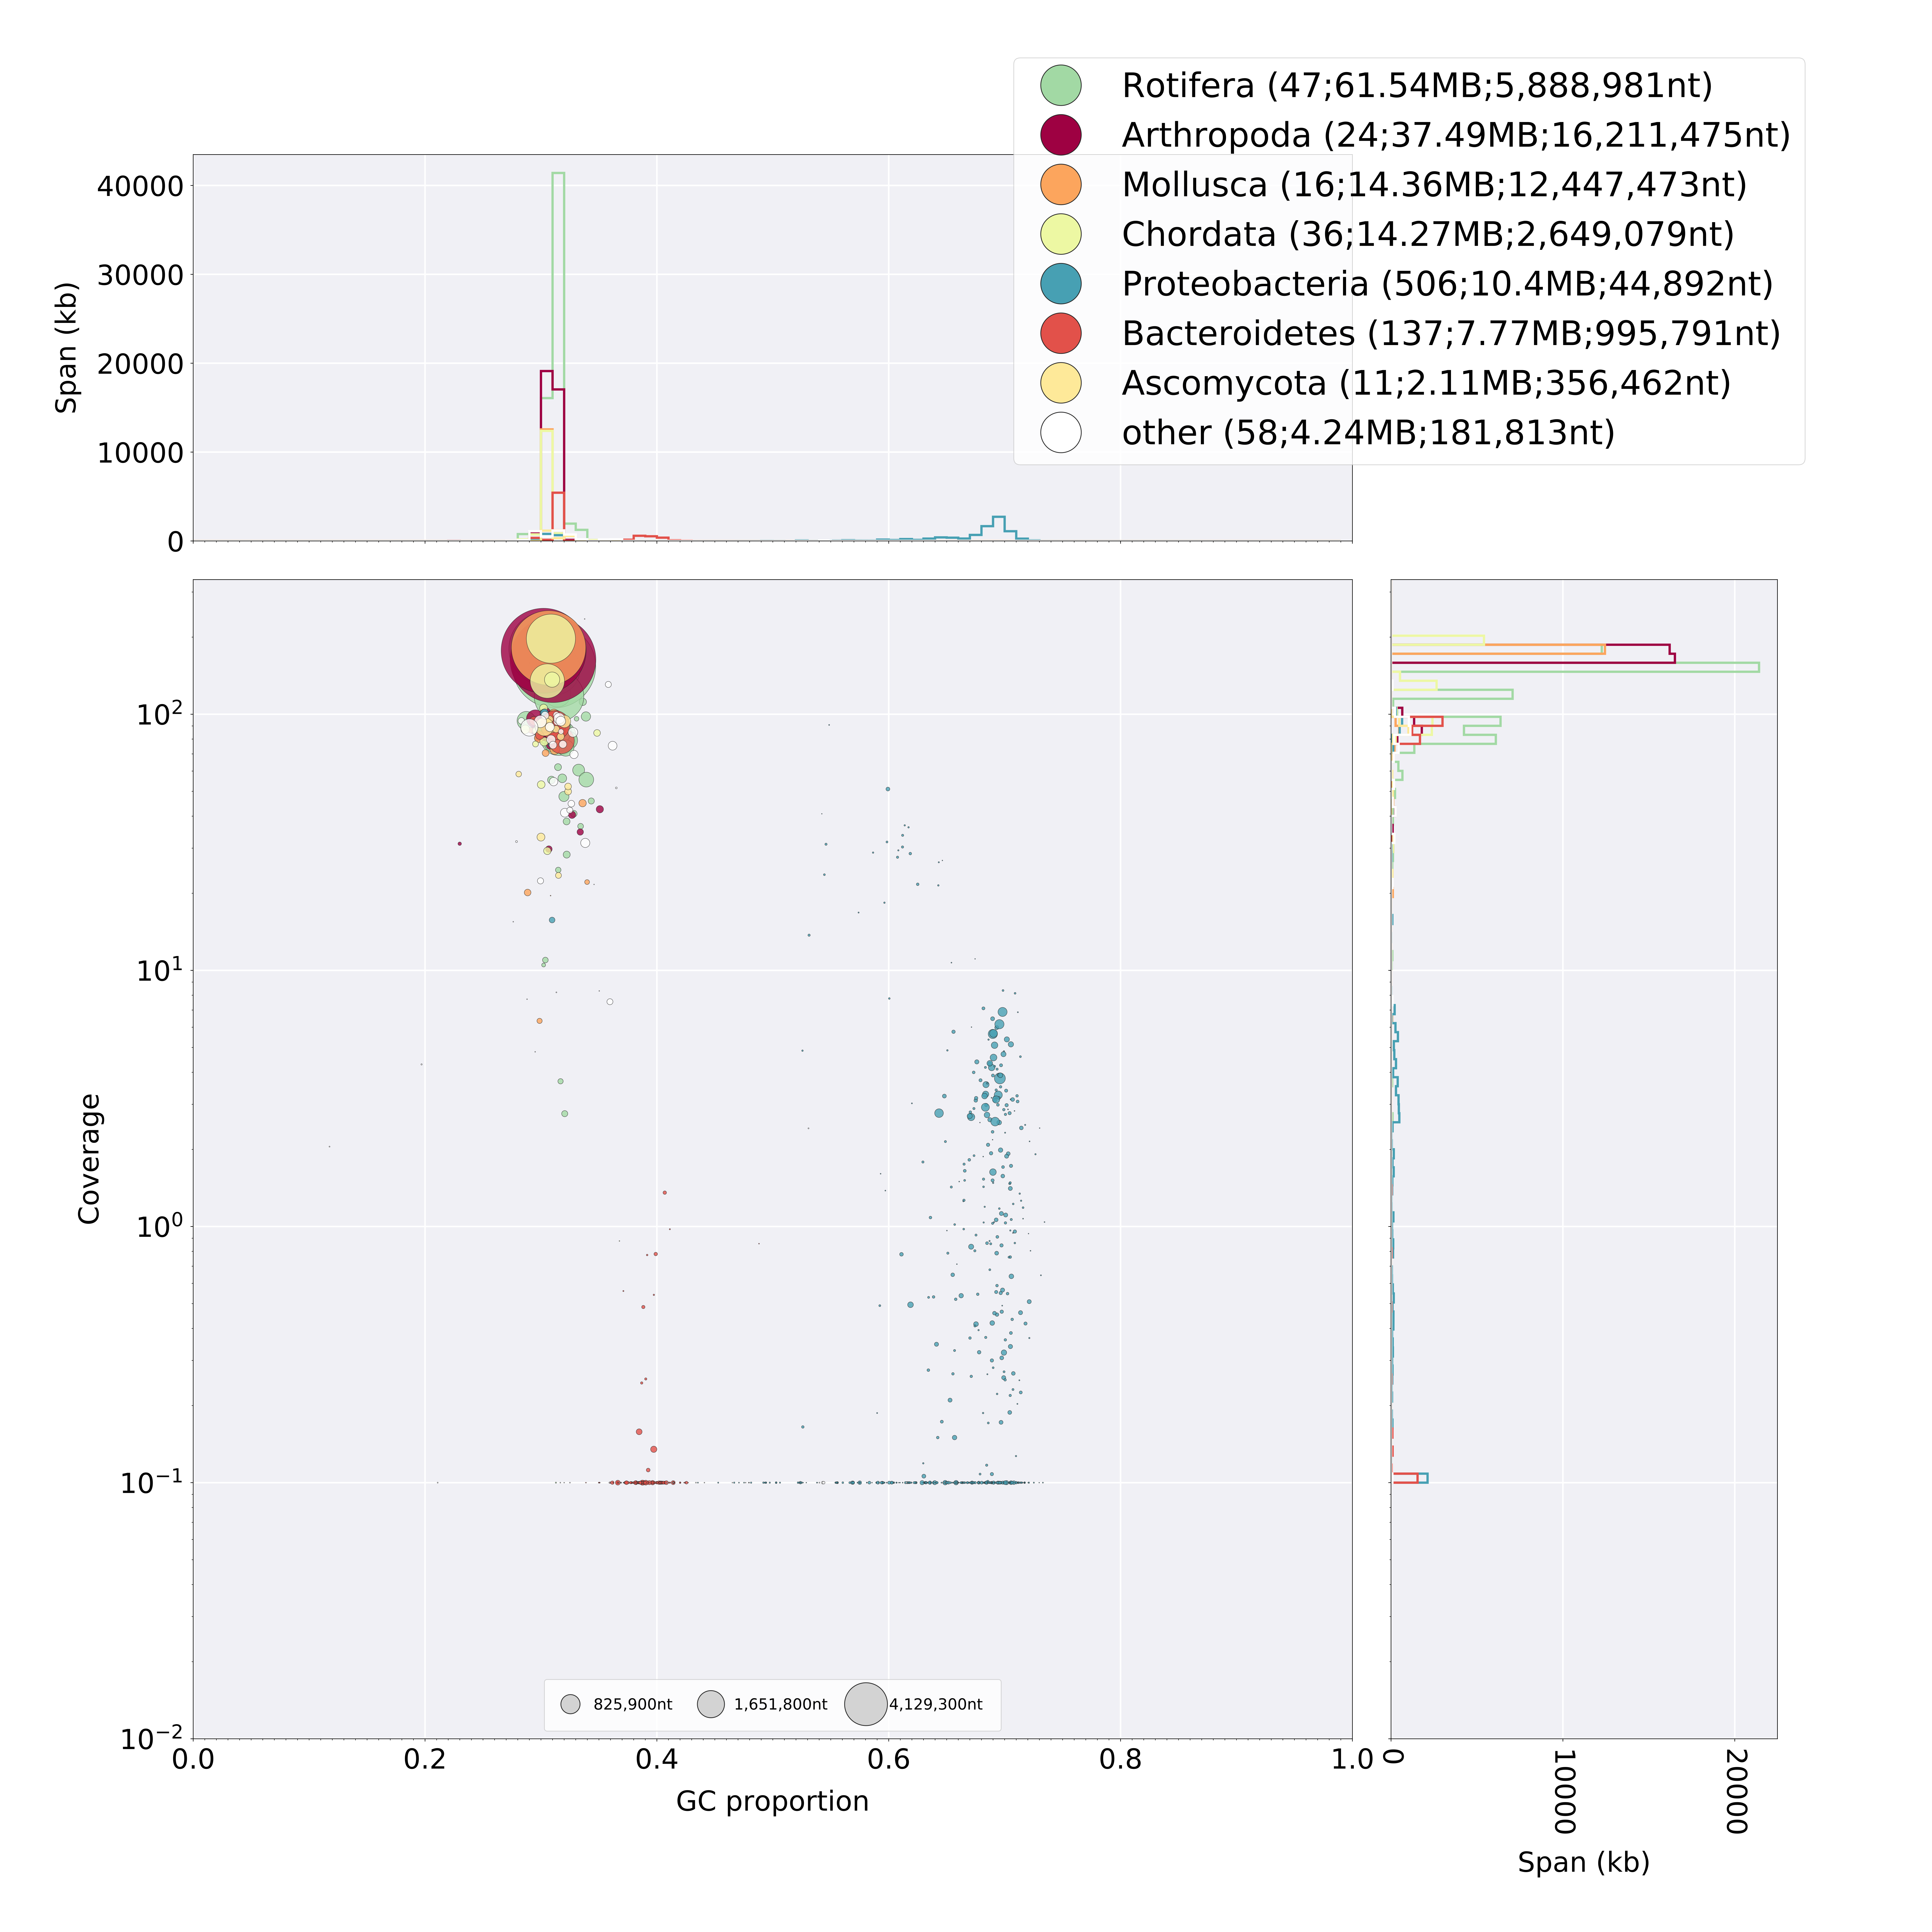
\includegraphics[width=15cm]{fig/benchmark/ONT_CANU.png}
   \caption{Blobtools v1.0 analysis of a Canu assembly of the full Nanopore dataset.}
   \label{fig:blobtools_canu_ont}
 \end{figure}
 
   \begin{figure}[ht]
    \centering
     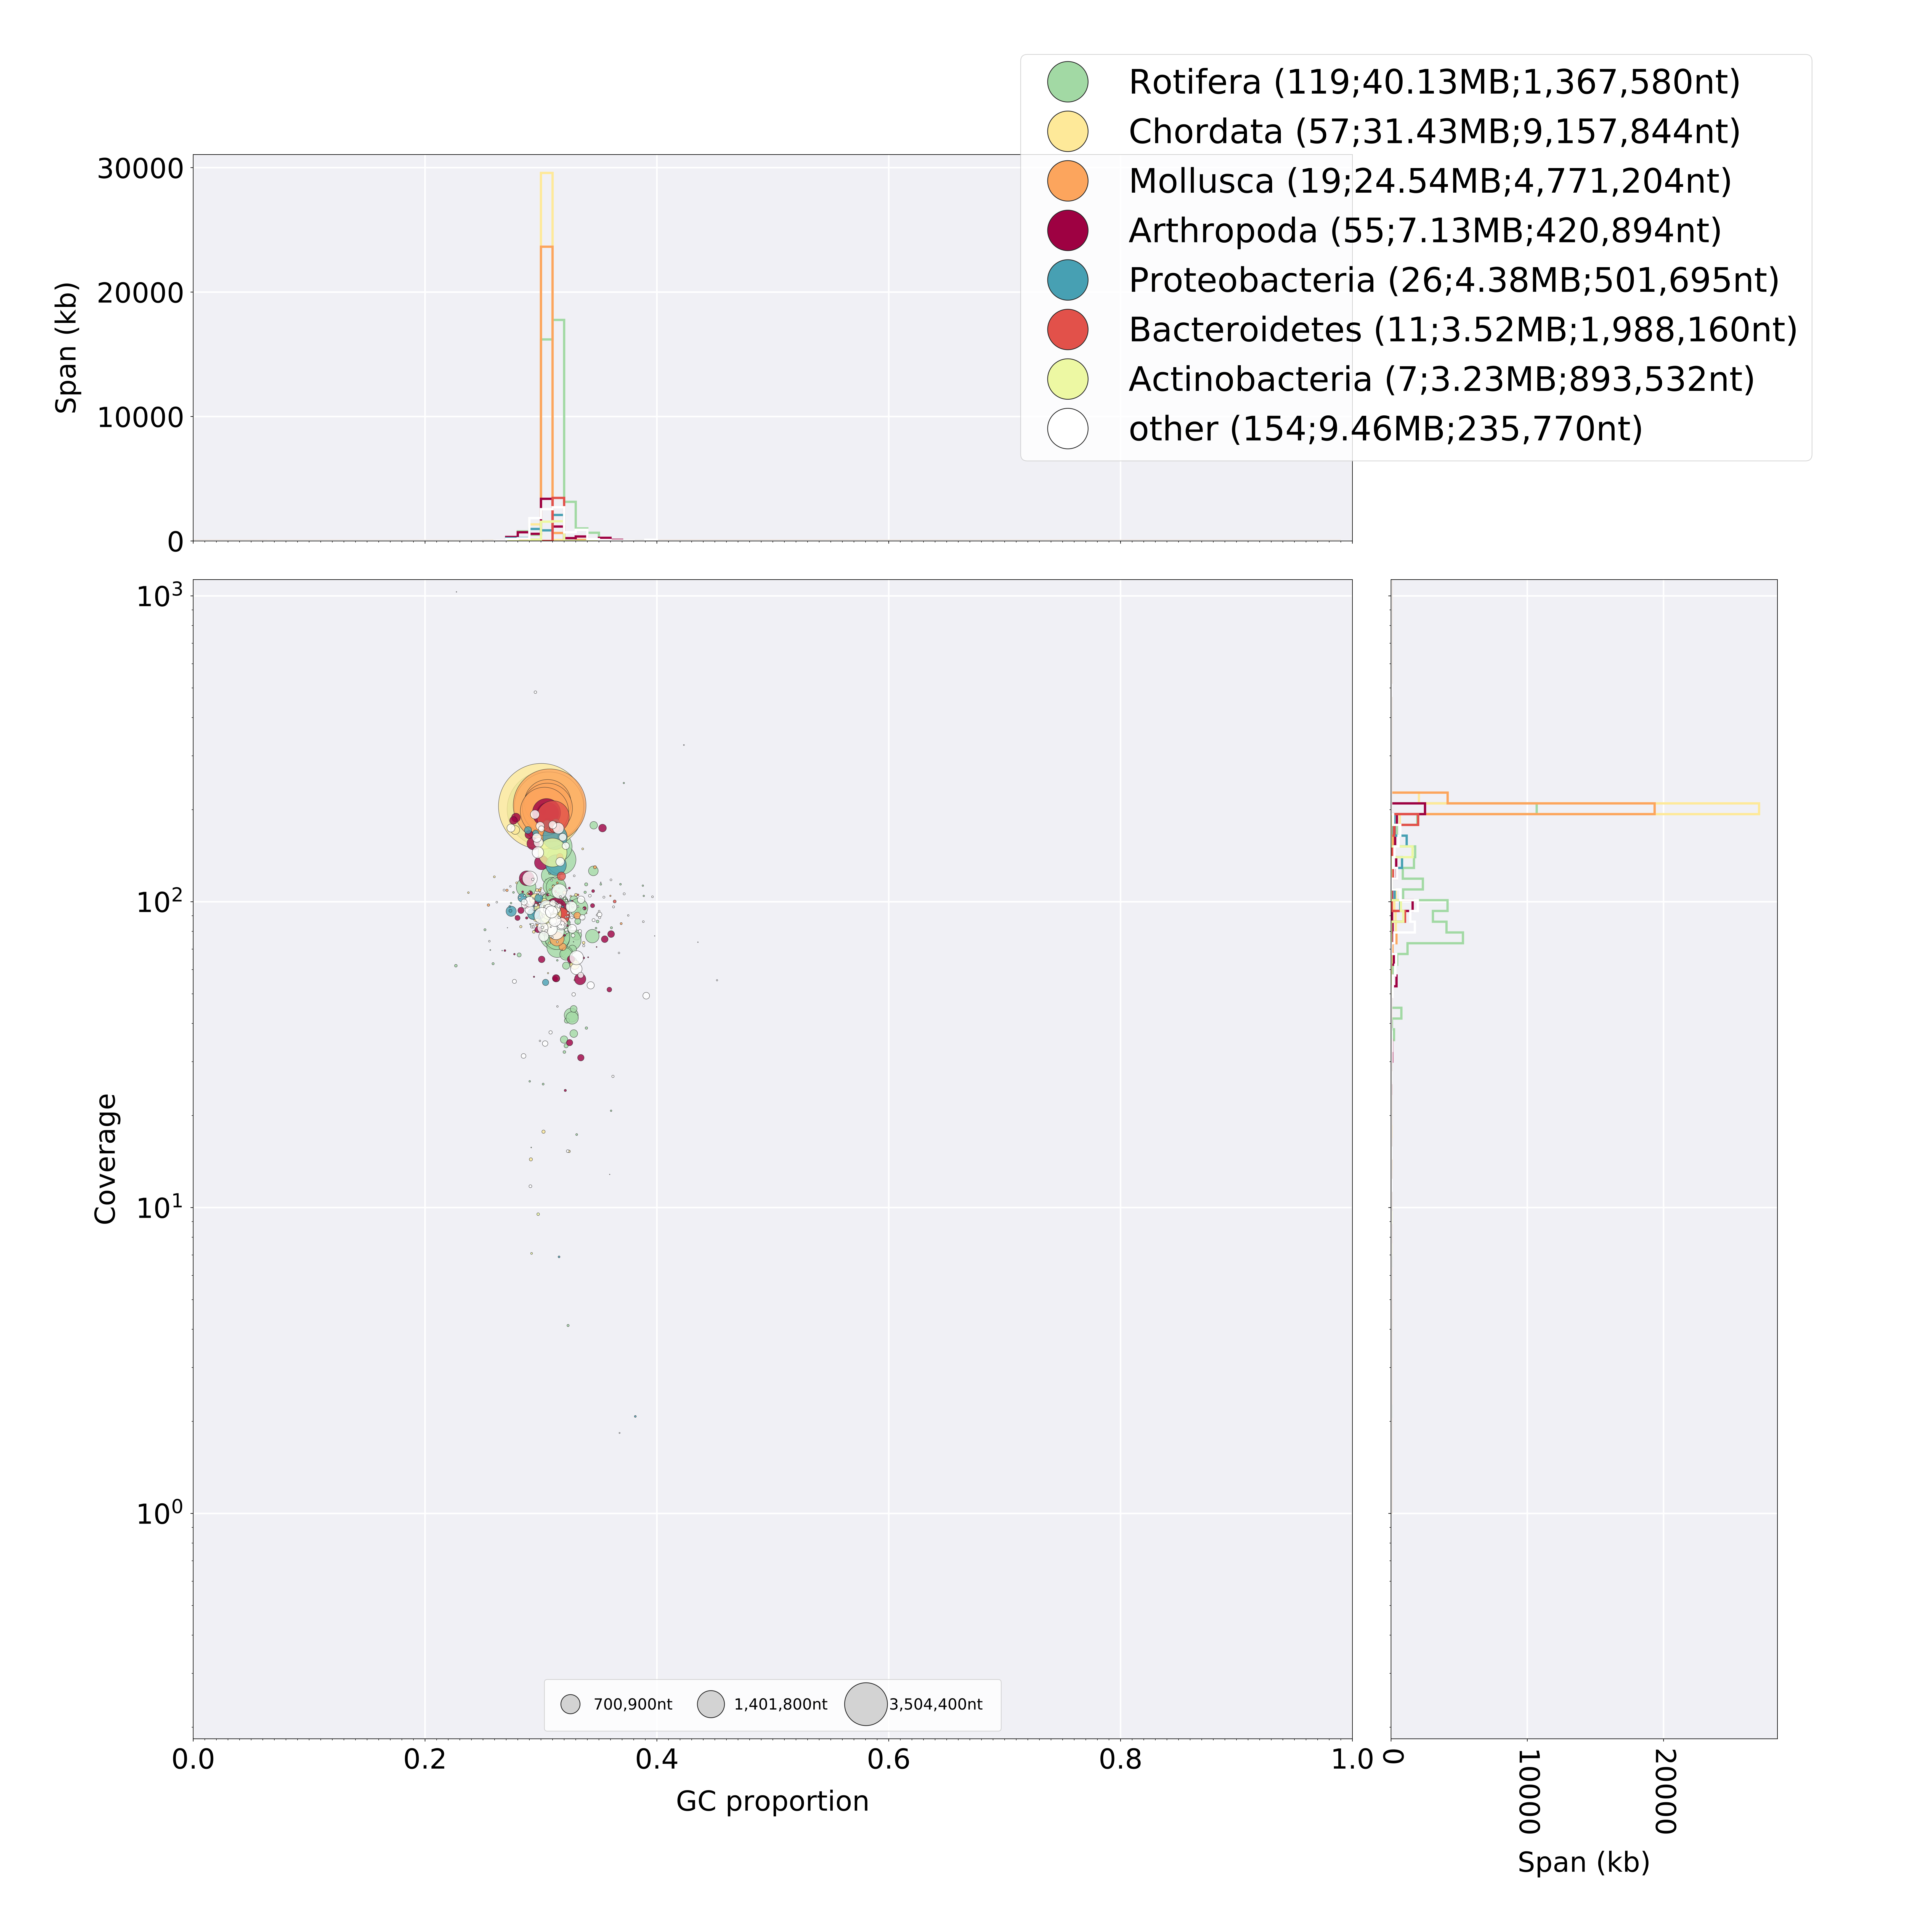
\includegraphics[width=15cm]{fig/benchmark/ONT_FLYE.png}
   \caption{Blobtools v1.0 analysis of a Flye assembly of the full Nanopore dataset.}
   \label{fig:blobtools_flye_ont}
 \end{figure}

  \begin{figure}[ht]
    \centering
     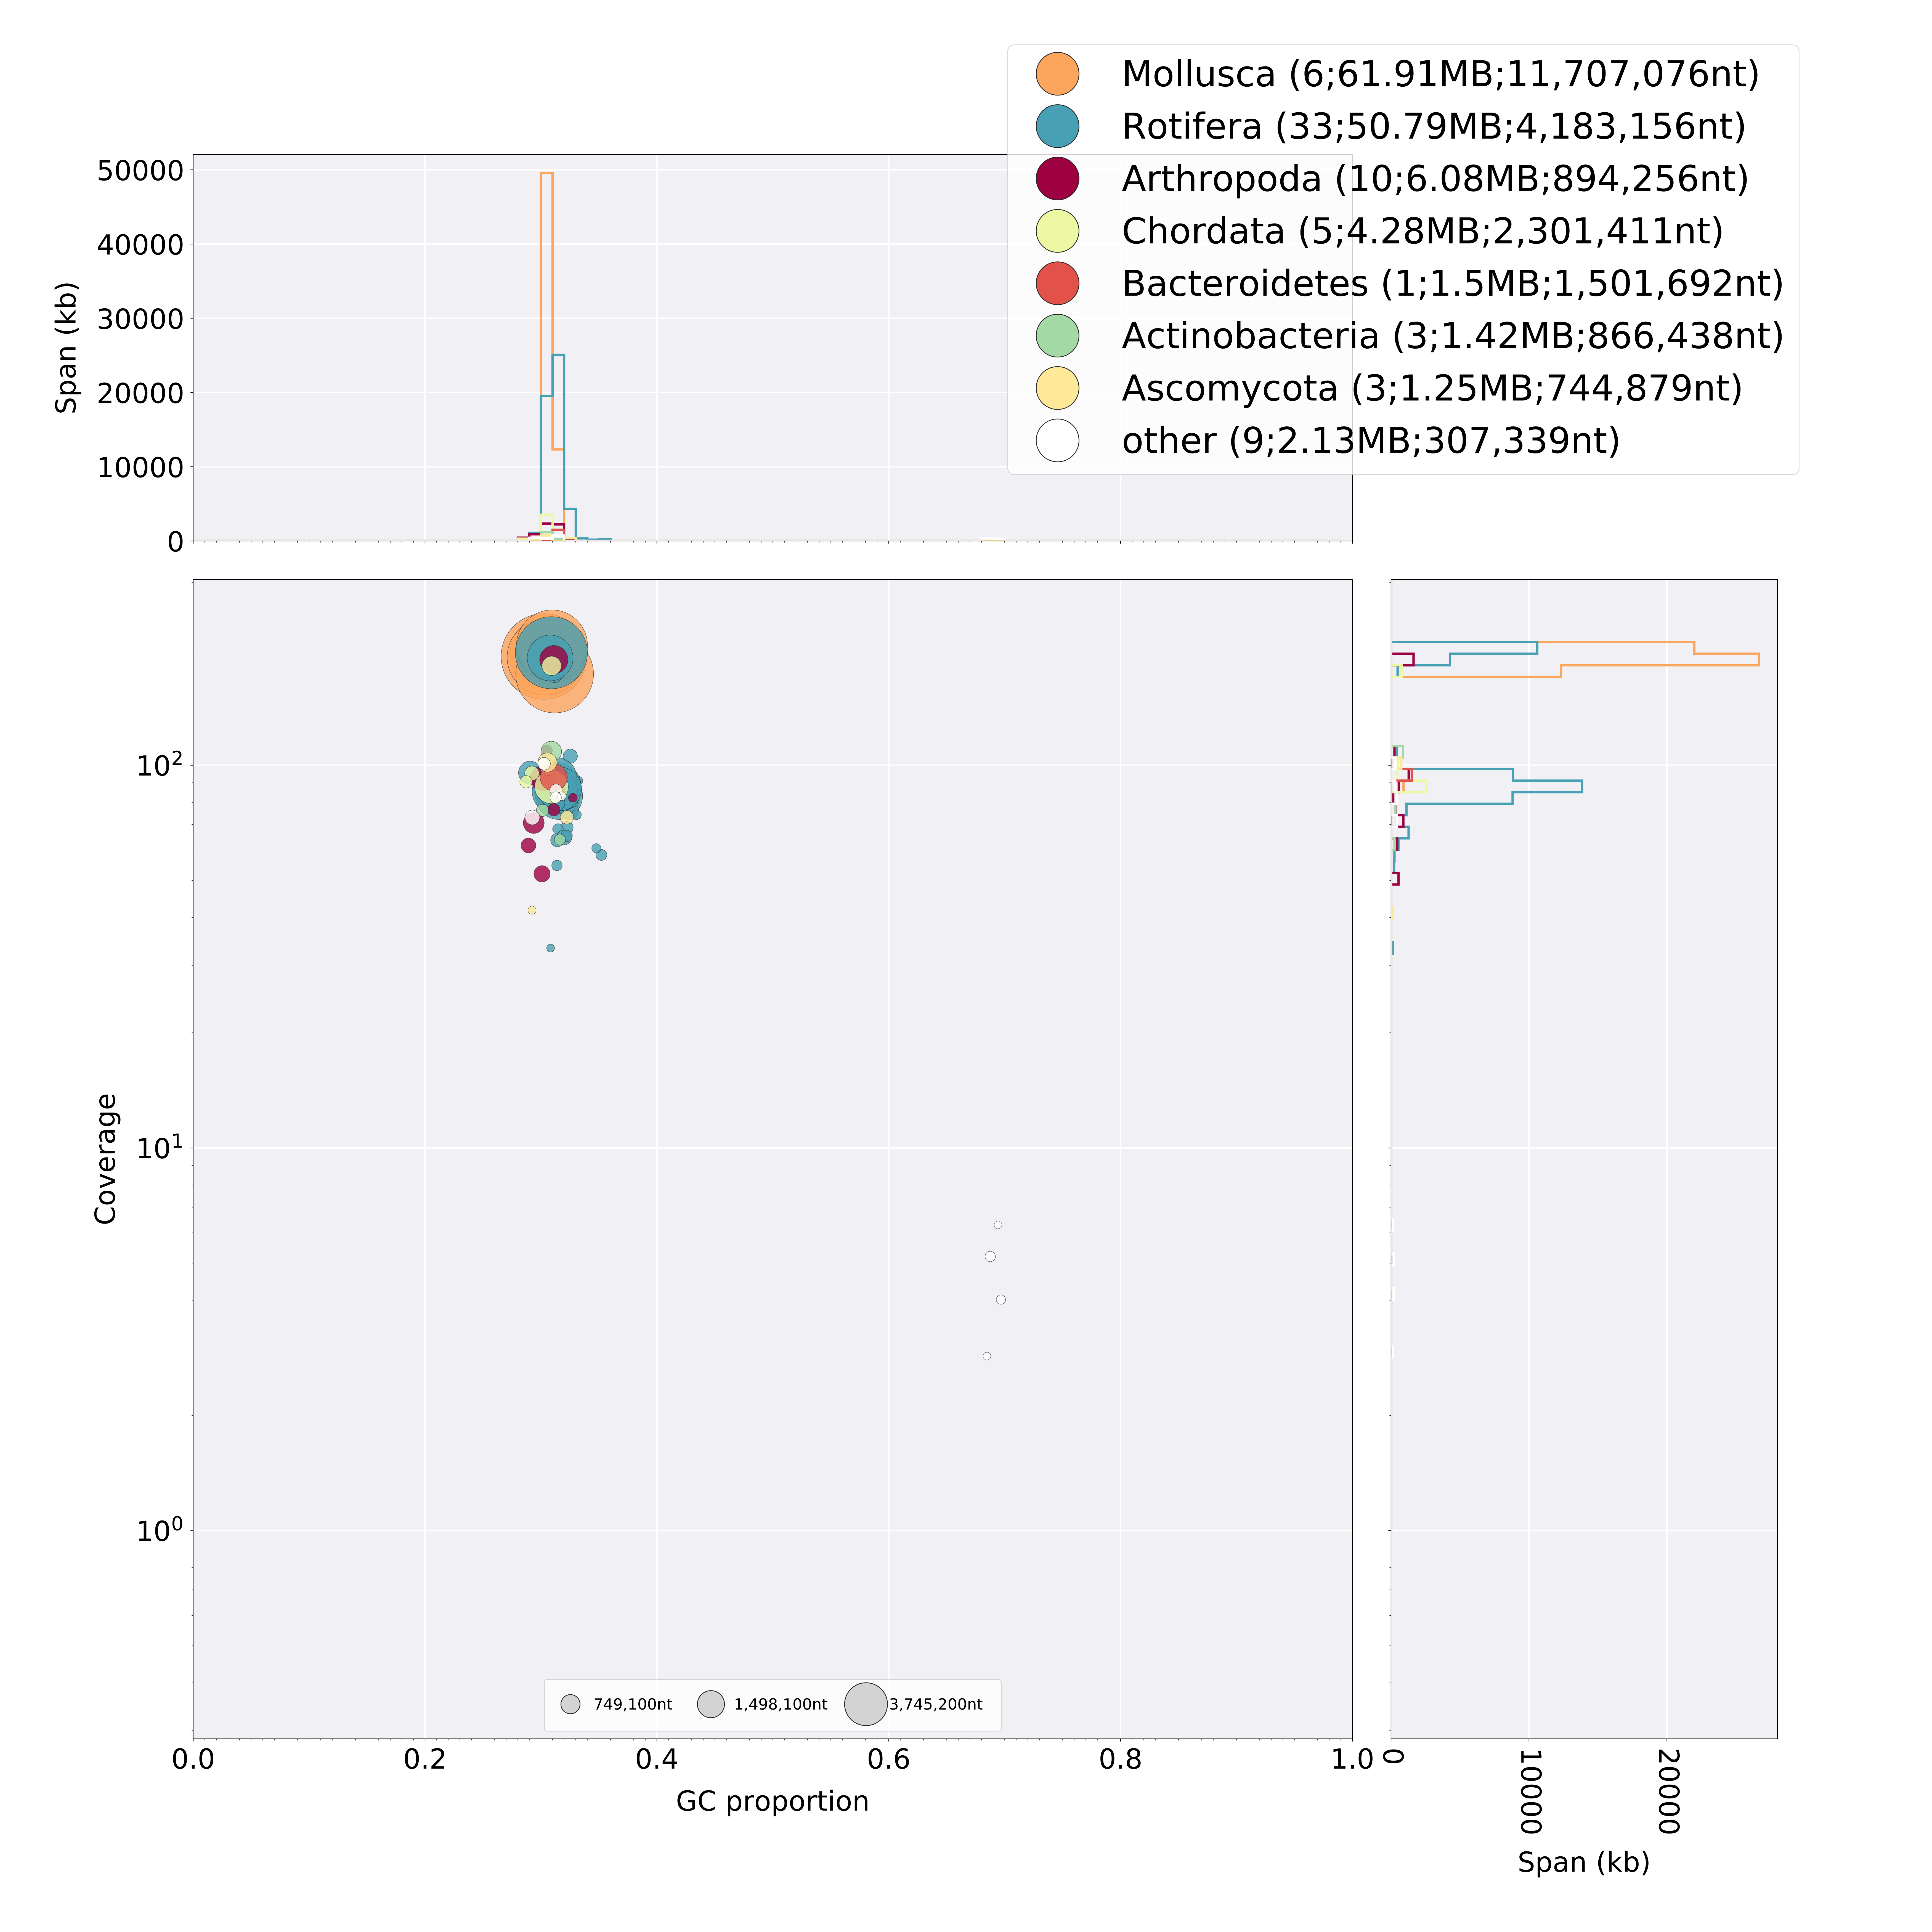
\includegraphics[width=15cm]{fig/benchmark/ONT_ND.png}
   \caption{Blobtools v1.0 analysis of a NextDenovo assembly of the full Nanopore dataset.}
   \label{fig:blobtools_NextDenovo_ont}
 \end{figure}

  \begin{figure}[ht]
    \centering
     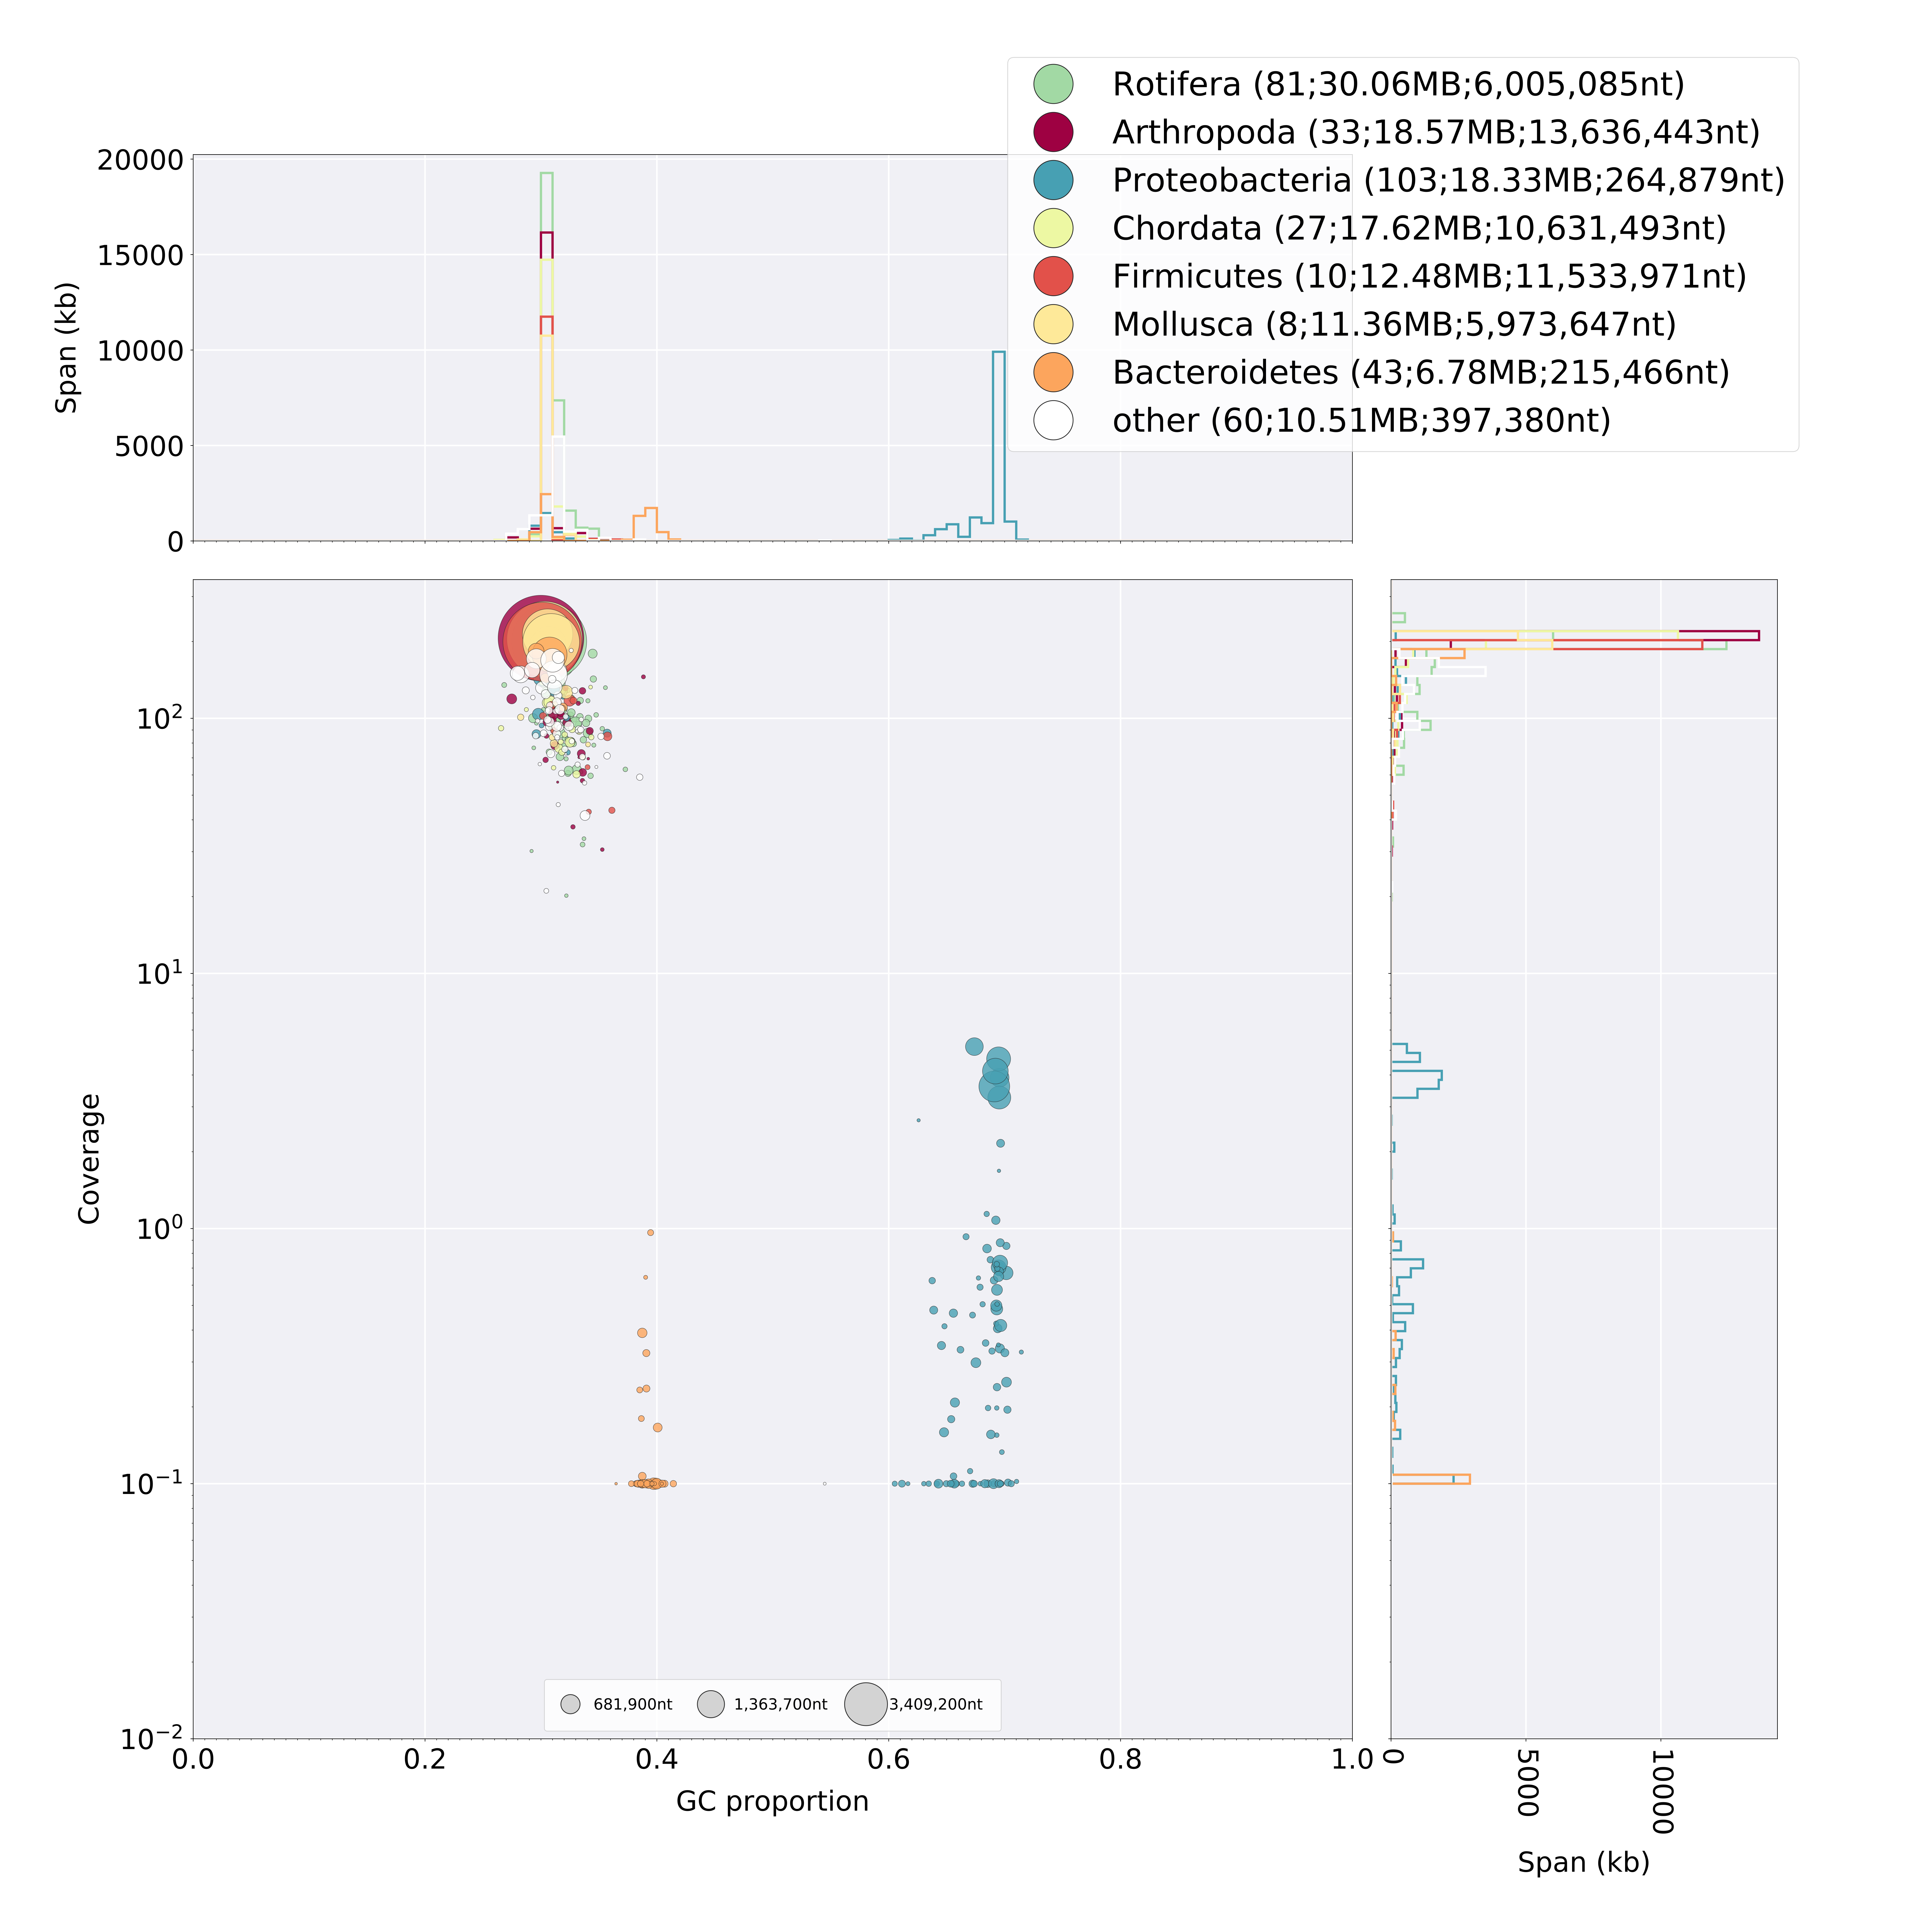
\includegraphics[width=15cm]{fig/benchmark/ONT_RA.png}
   \caption{Blobtools v1.0 analysis of a Ra assembly of the full Nanopore dataset.}
   \label{fig:blobtools_ra_ont}
 \end{figure}

  \begin{figure}[ht]
    \centering
     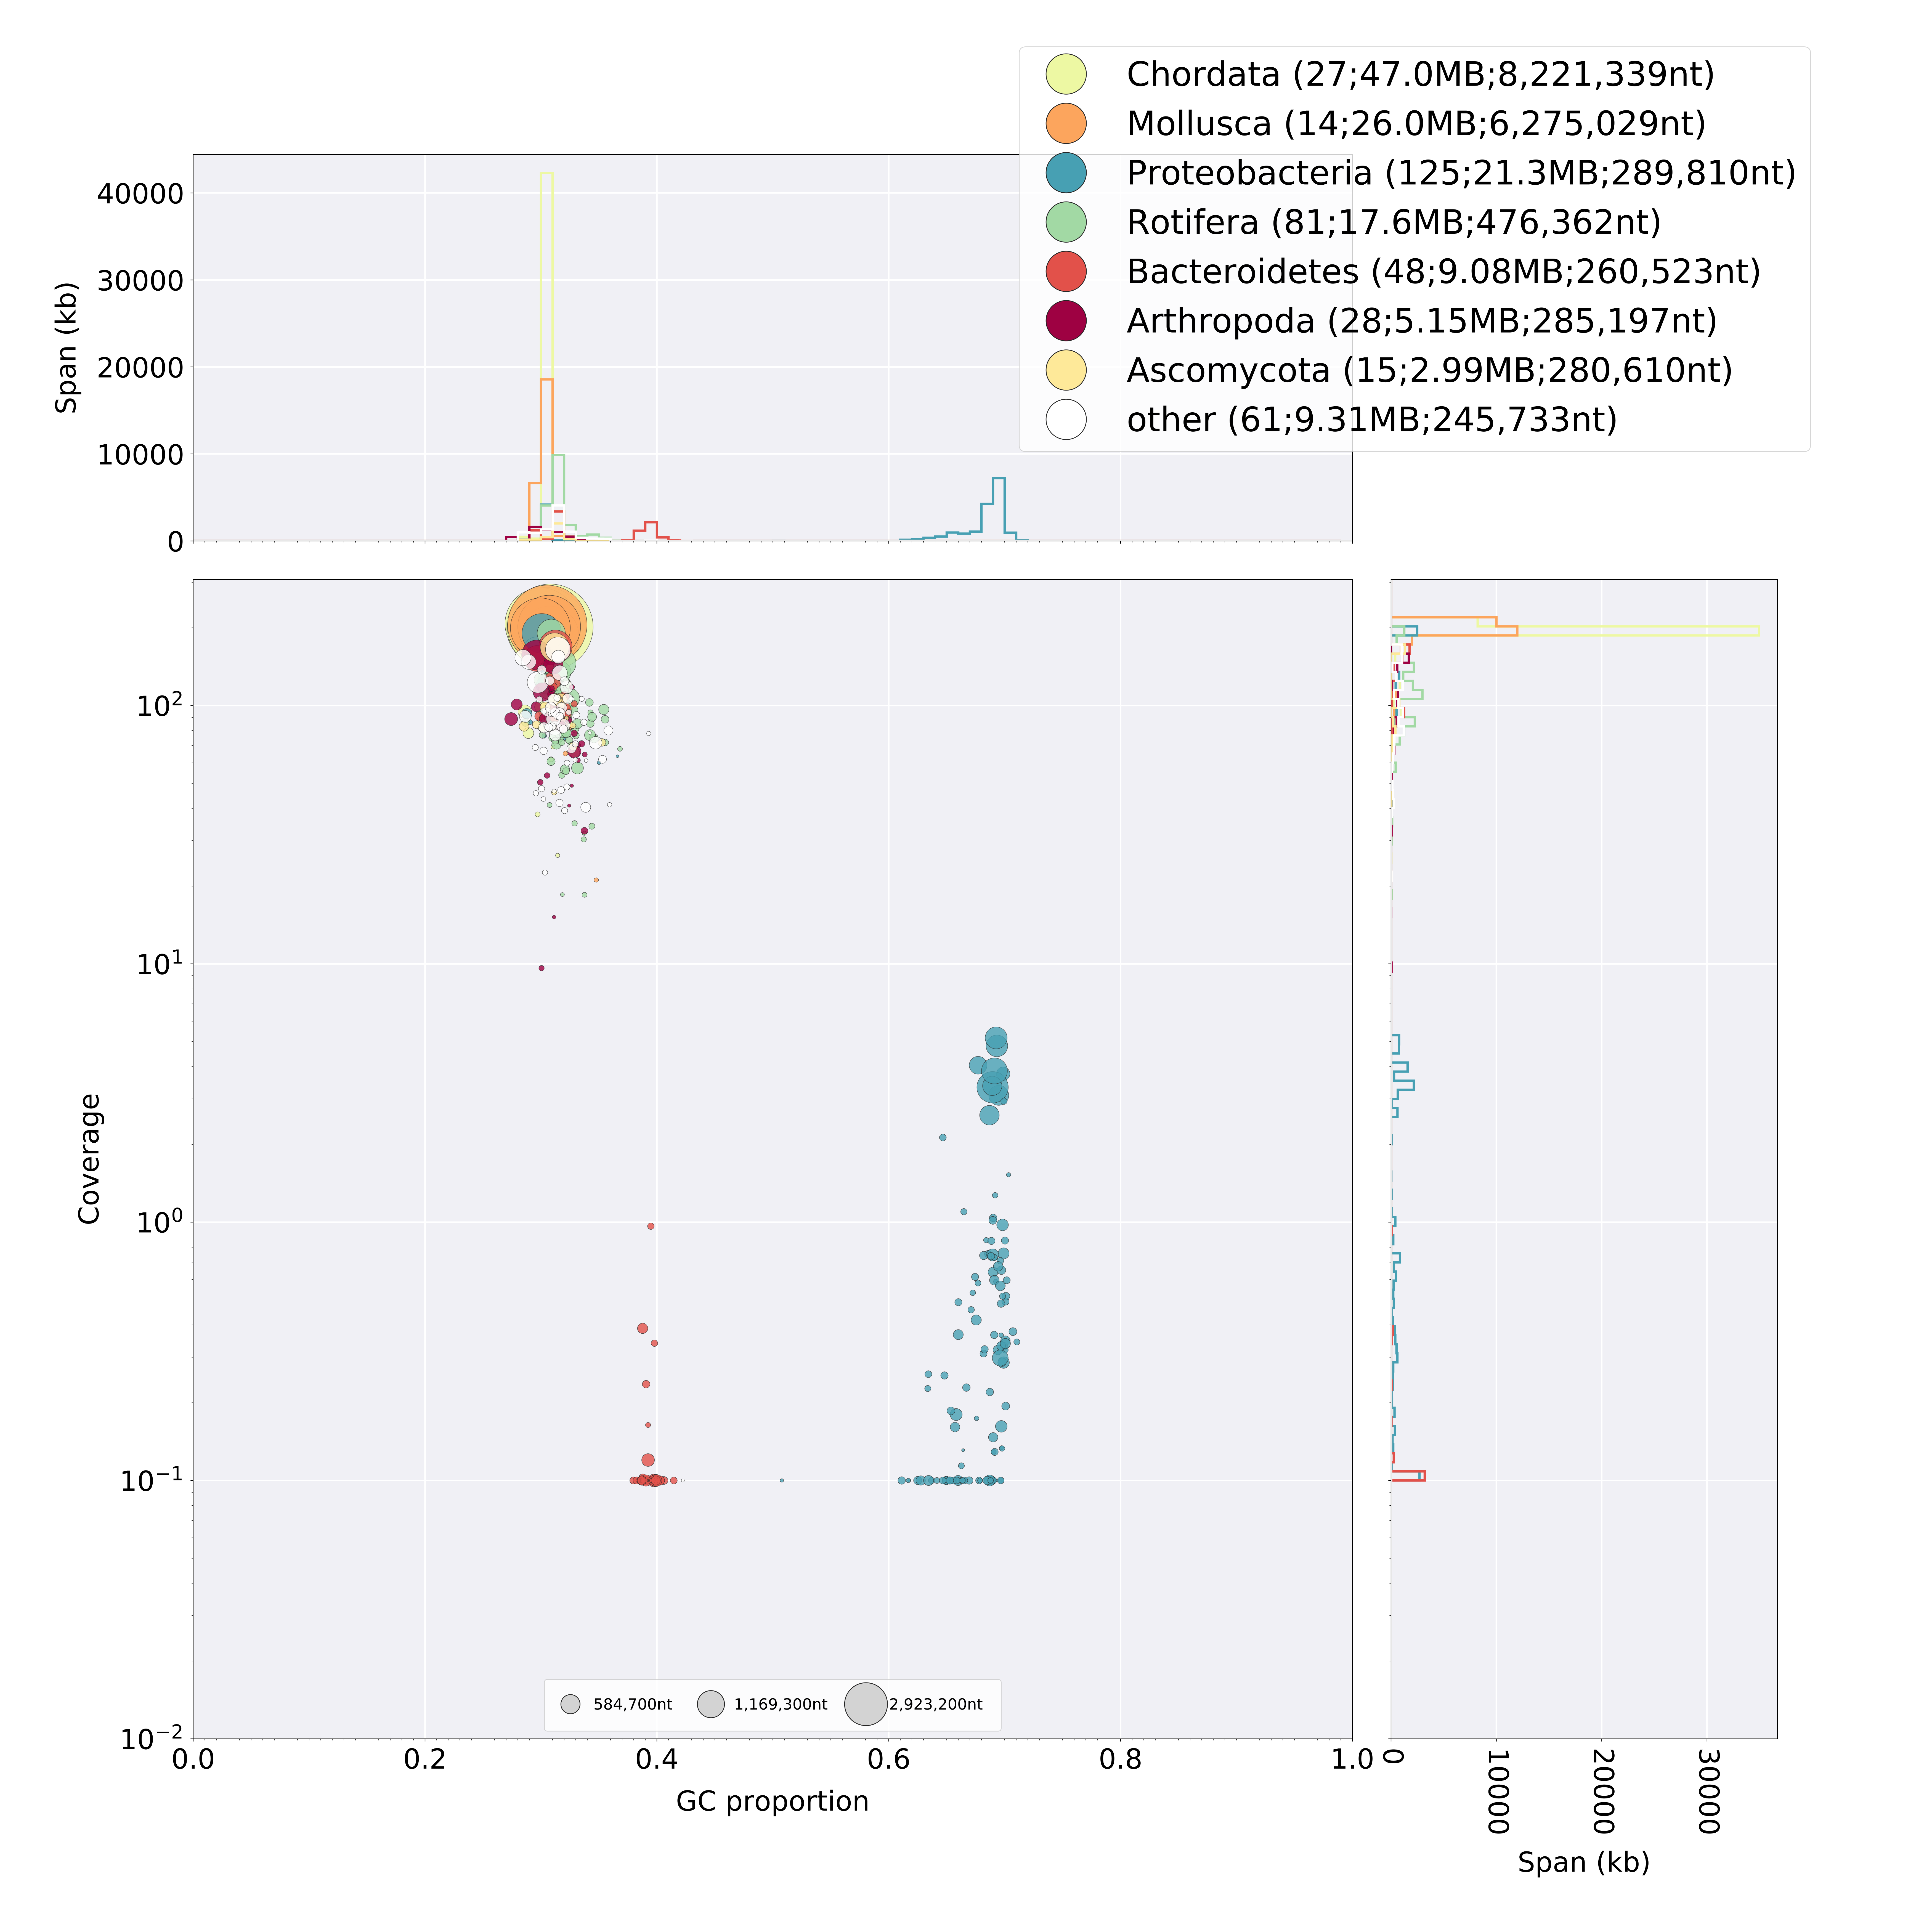
\includegraphics[width=15cm]{fig/benchmark/ONT_RAVEN.png}
   \caption{Blobtools v1.0 analysis of a Raven assembly of the full Nanopore dataset.}
   \label{fig:blobtools_raven_ont}
 \end{figure}

  \begin{figure}[ht]
    \centering
     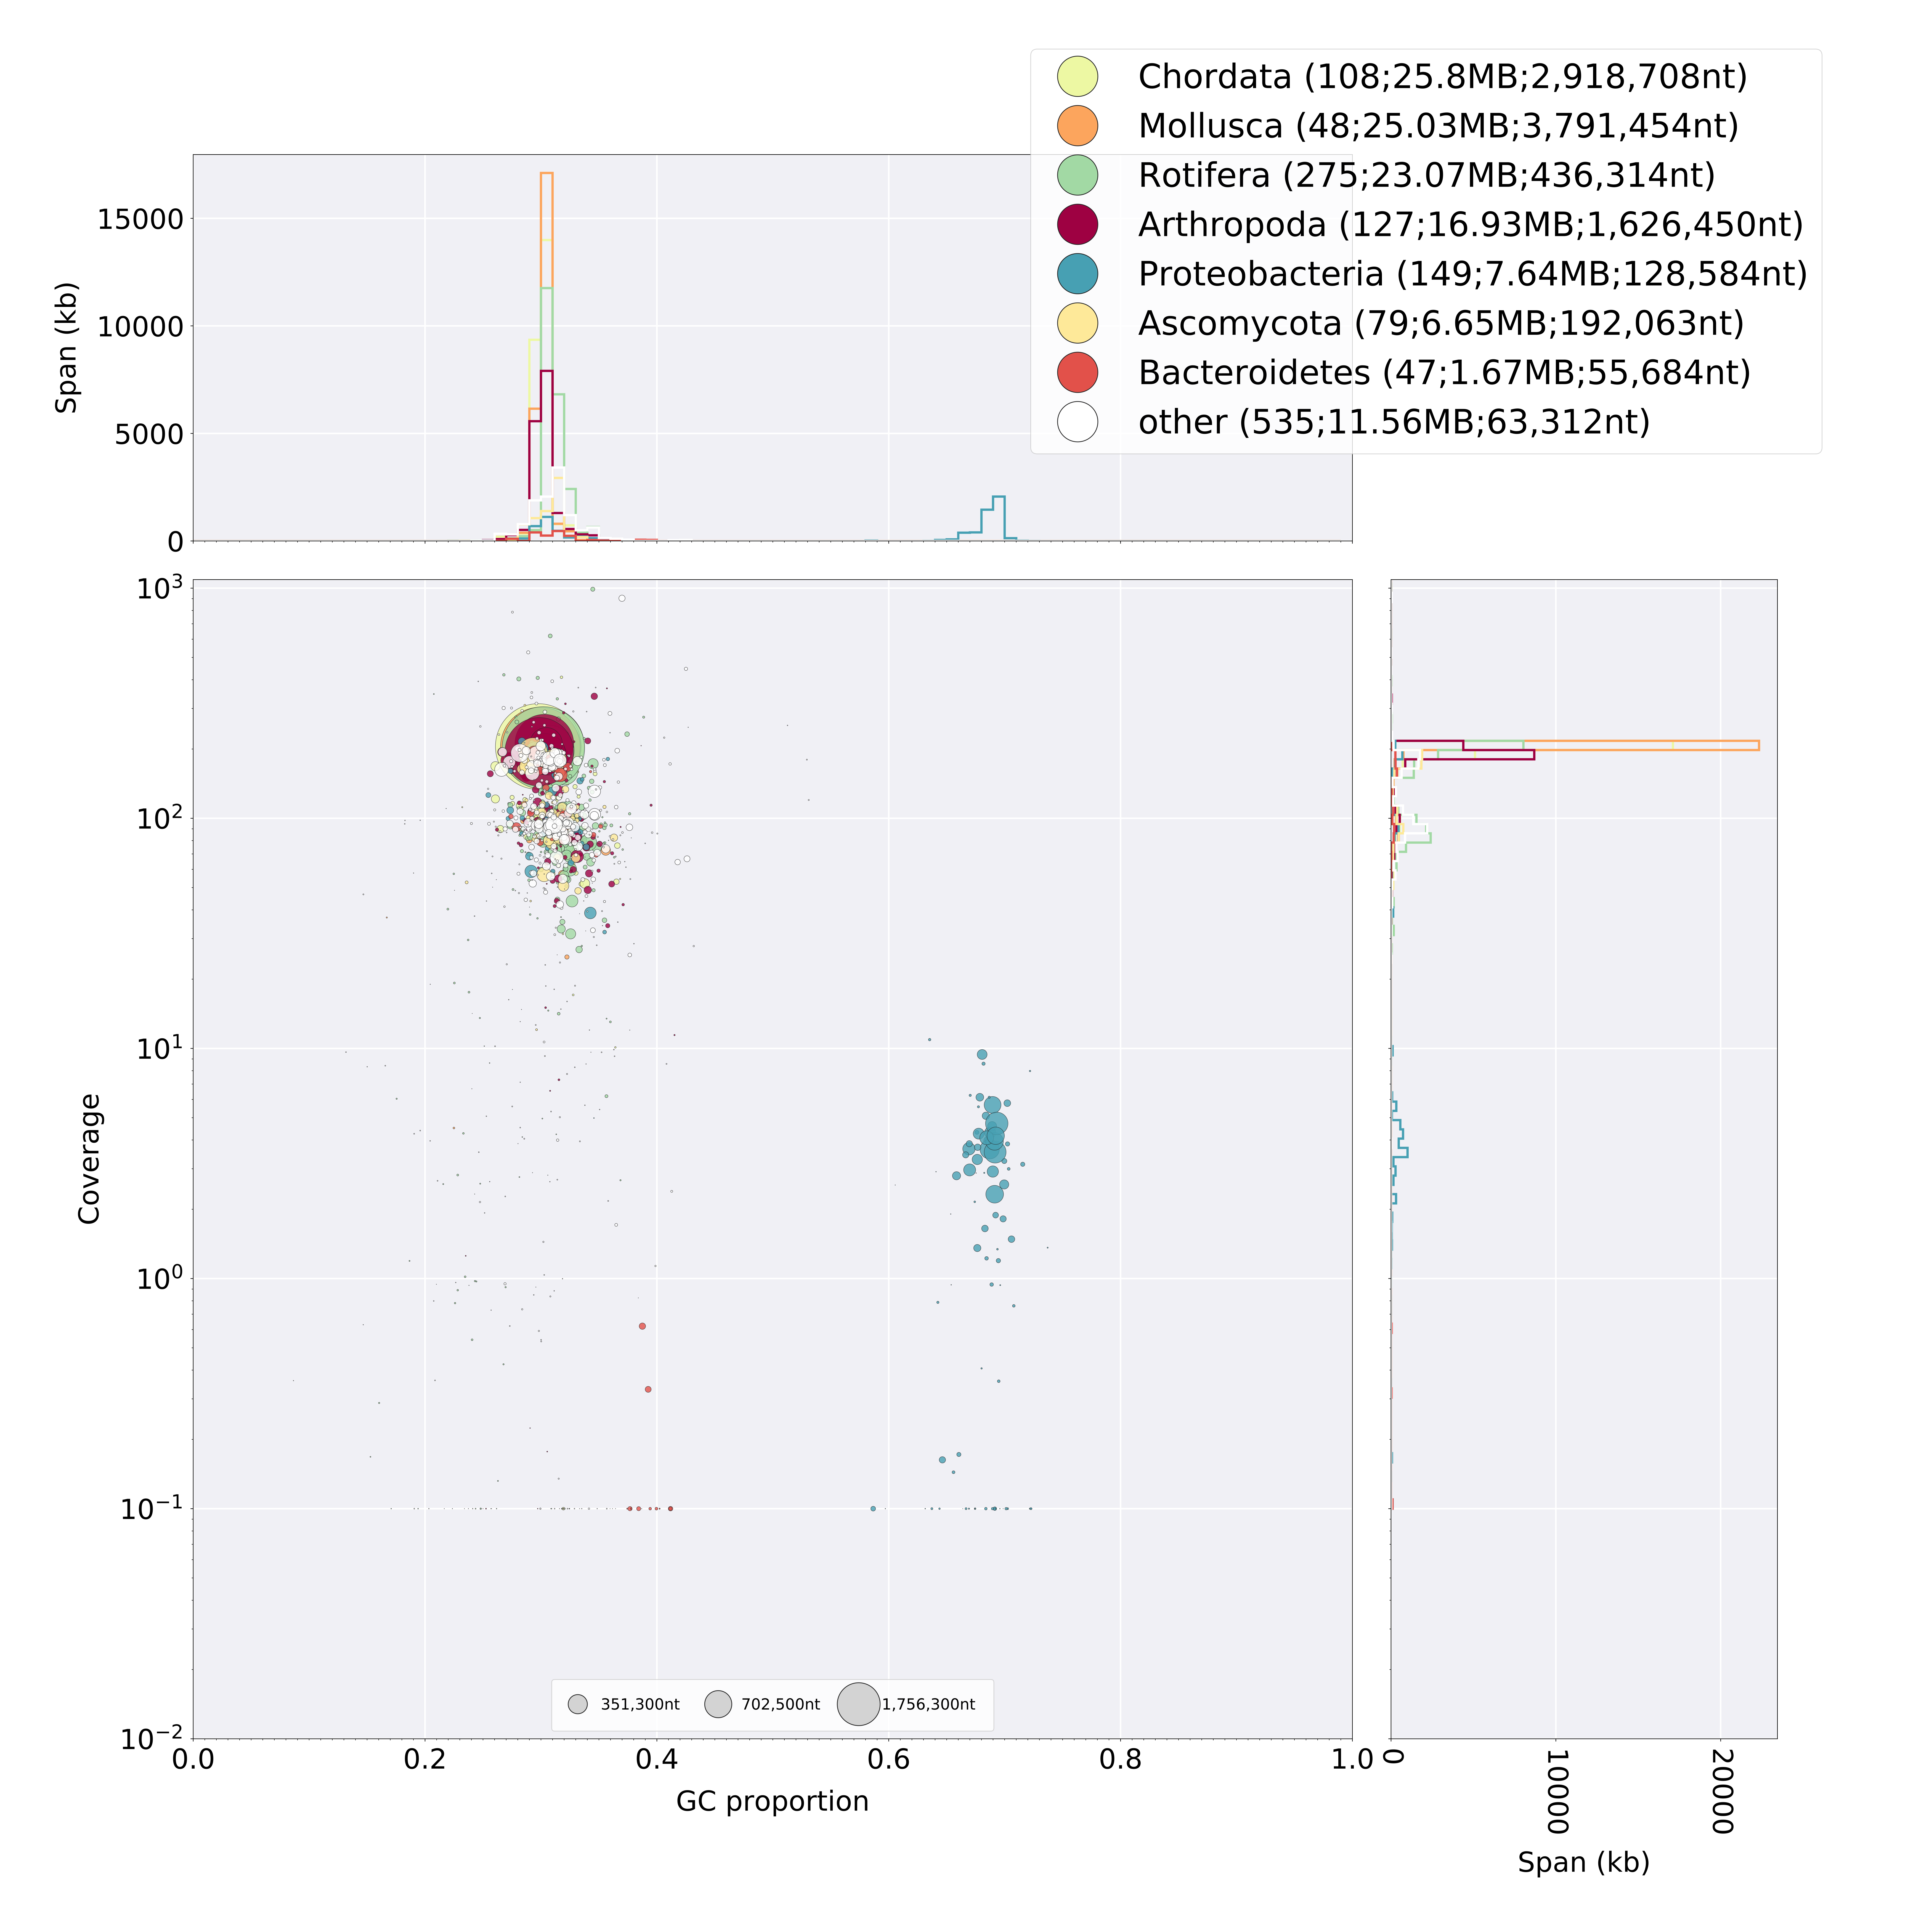
\includegraphics[width=15cm]{fig/benchmark/ONT_SHASTA.png}
   \caption{Blobtools v1.0 analysis of a Shasta assembly of the full Nanopore dataset.}
   \label{fig:blobtools_shasta_ont}
 \end{figure}

 \begin{figure}[ht]
    \centering
     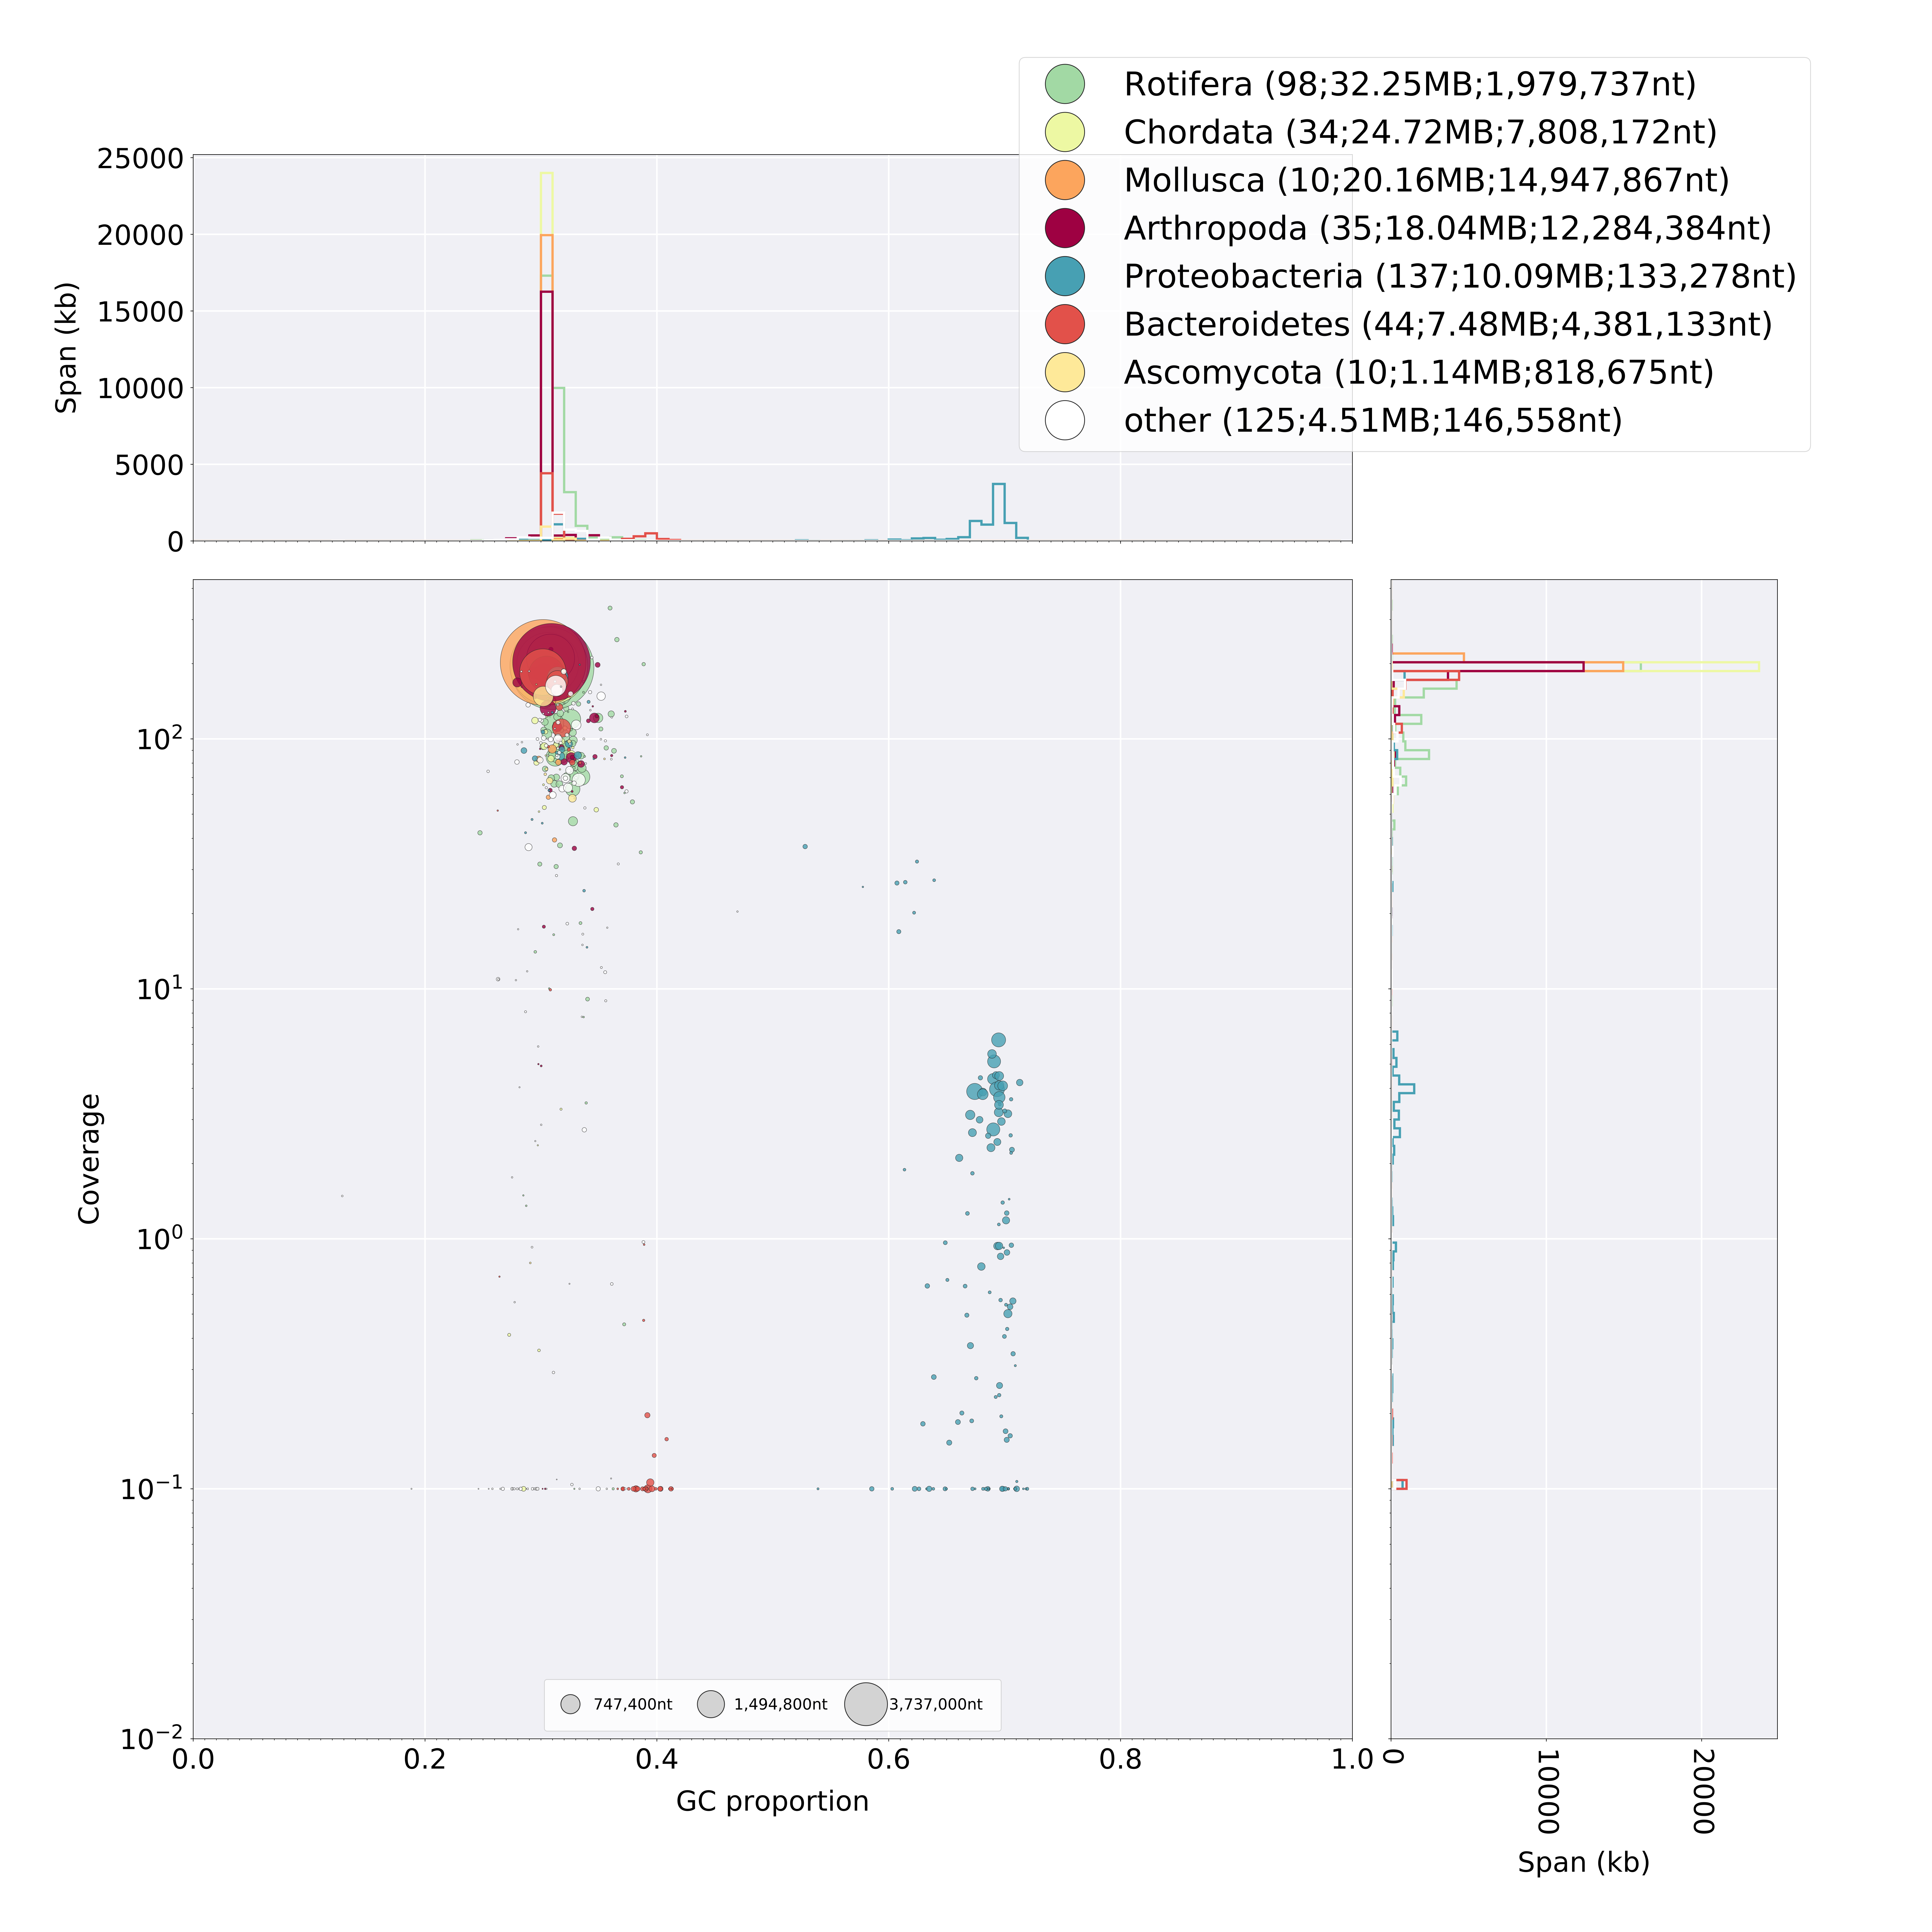
\includegraphics[width=15cm]{fig/benchmark/ONT_WTDBG.png}
   \caption{Blobtools v1.0 analysis of a wtdbg2 assembly of the full Nanopore dataset.}
   \label{fig:blobtools_wtdbg_ont}
 \end{figure}


     \begin{figure}[ht]
    \centering
     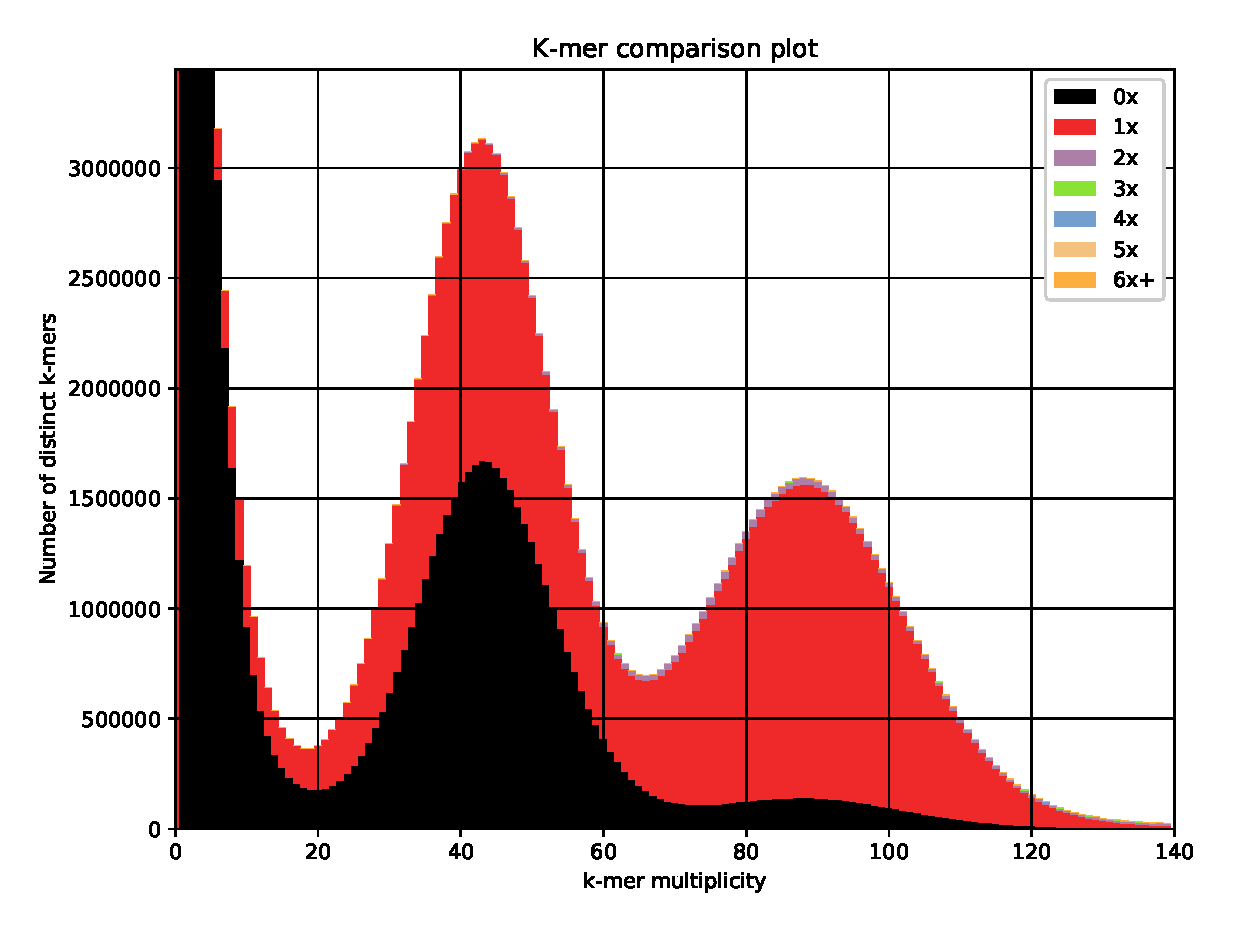
\includegraphics[width=13.5cm]{fig/benchmark/kat_comp_shasta_1-main.mx.spectra-cn.eps}
   \caption{\textit{k}-mer spectrum of the Shasta assembly of the full Nanopore dataset obtained with KAT v2.4.2.}
   \label{fig:kat_shasta_all}
 \end{figure}
 
    \begin{figure}[ht]
    \centering
     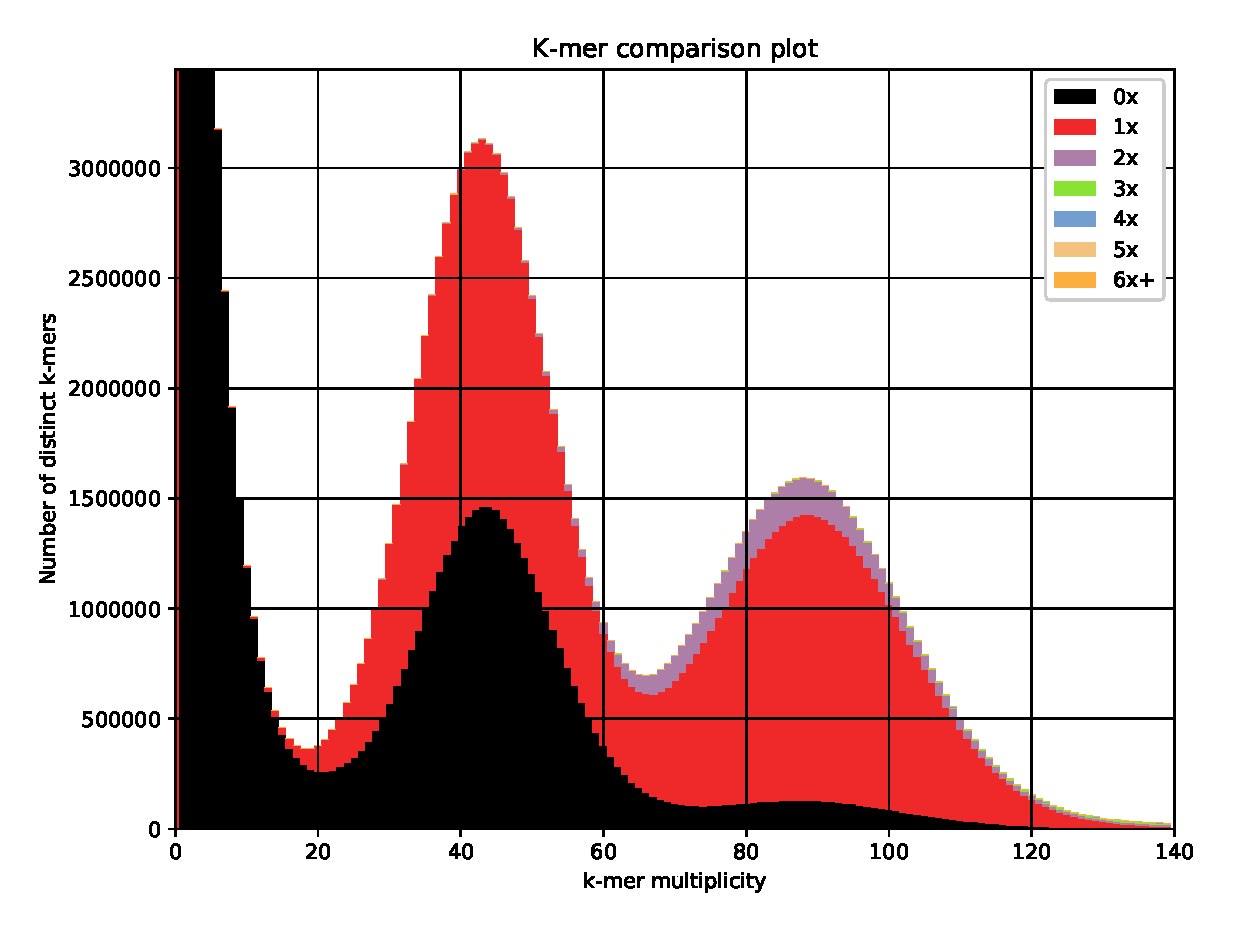
\includegraphics[width=13.5cm]{fig/benchmark/kat_comp_shasta_min30000_1-main.mx.spectra-cn.eps}
   \caption{\textit{k}-mer spectrum of the Shasta assembly of the longest Nanopore reads obtained with KAT v2.4.2.}
   \label{fig:kat_shasta_min30000}
 \end{figure}
 
    \begin{figure}[ht]
    \centering
     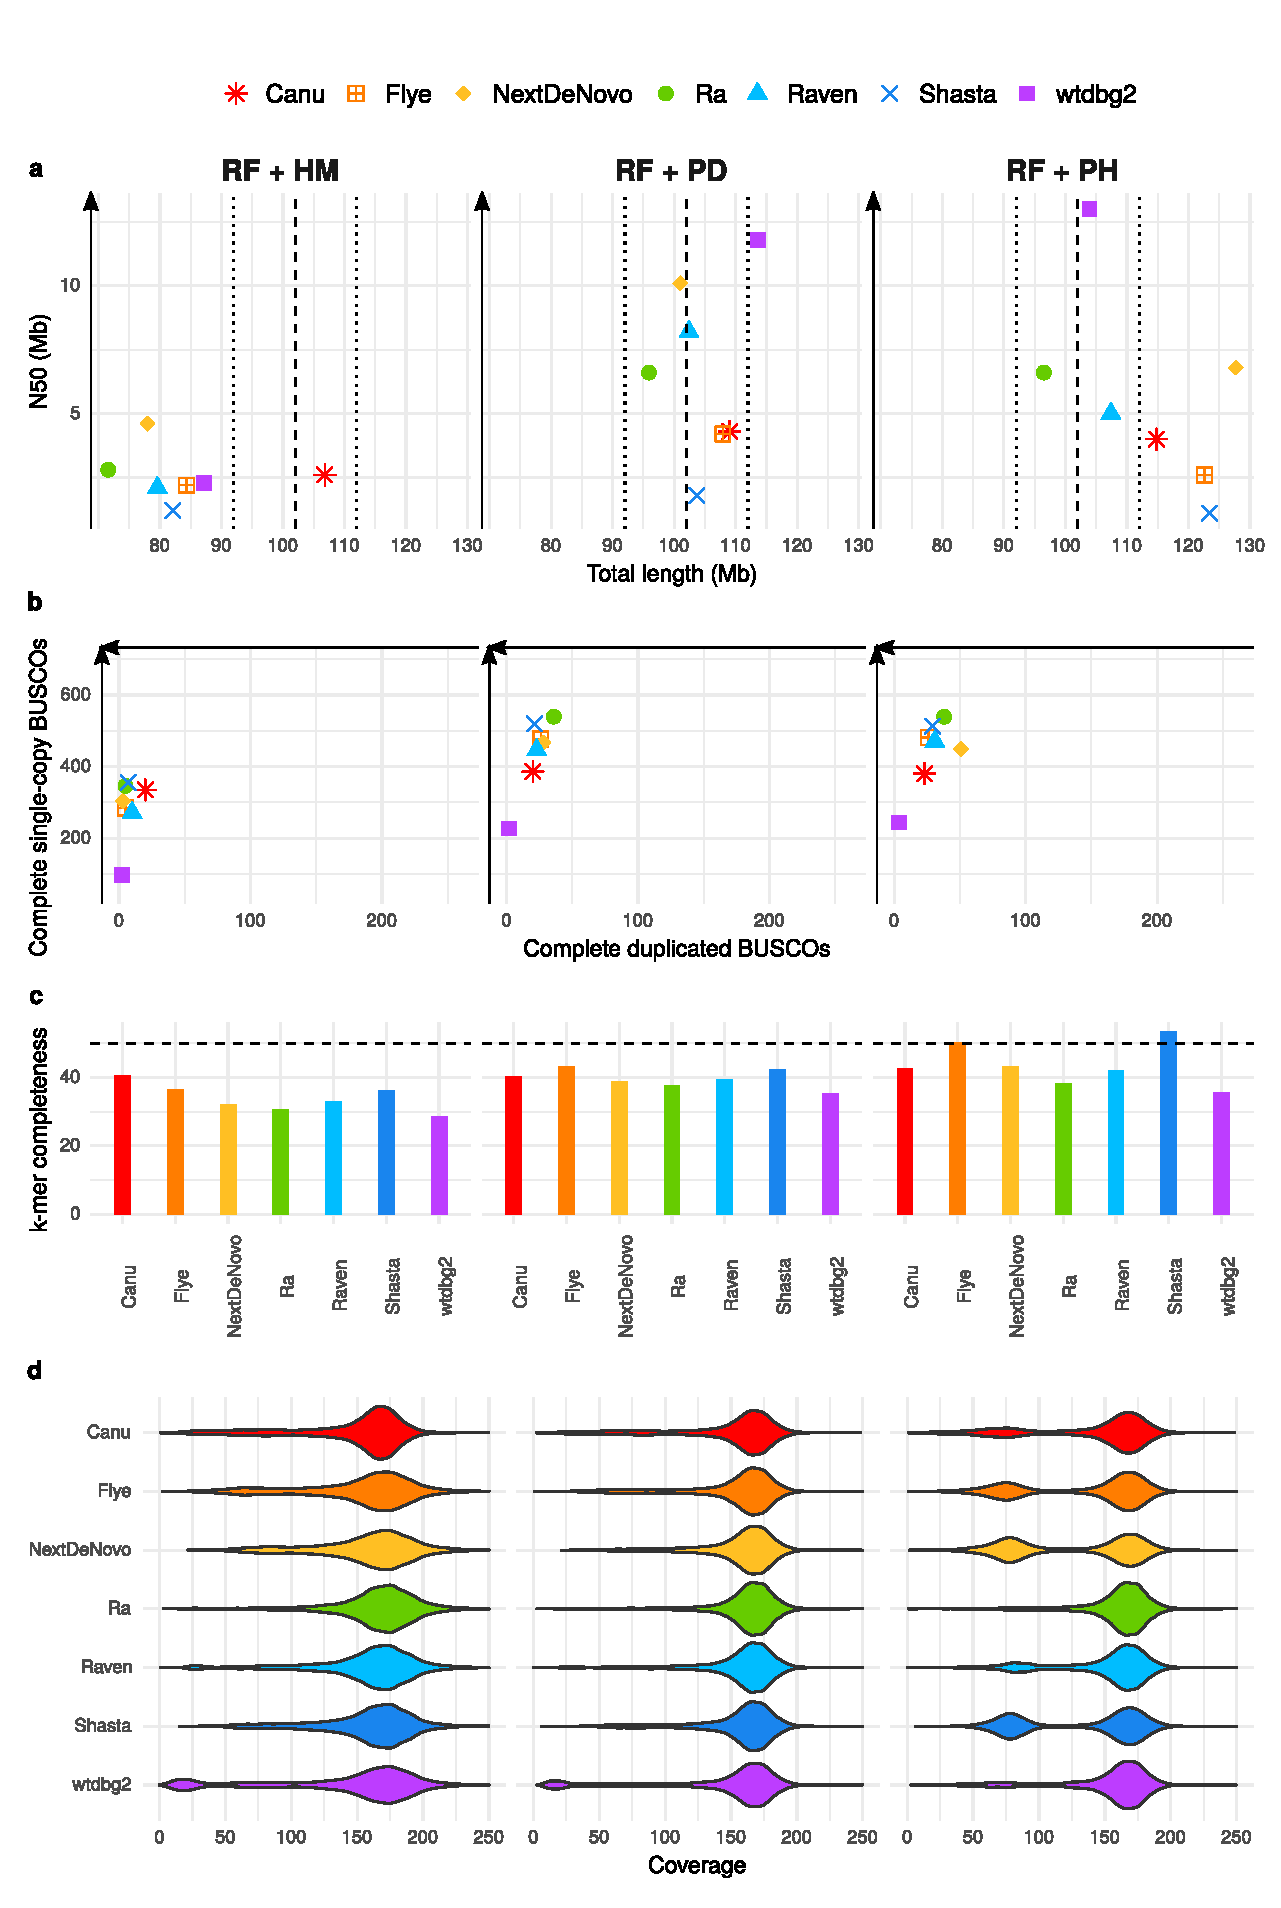
\includegraphics[width=13.5cm]{fig/benchmark/supp_nanopore_filtering_purging_v20201012.eps}
   \caption{Statistics of Nanopore assemblies obtained from the filtered Nanopore dataset of reads longer than 30 kb, with a subsequent removal of uncollapsed haplotypes with HaploMerger2 (HM), purge\_dups (PD), or purge\_haplotigs (PH). a) N50 plotted against total assembly length. The dashed line indicates the expected genome size, with a +/- 10 Mb margin delimited by the dotted lines. b) Number of complete single-copy BUSCOs plotted against number of complete duplicated BUSCOs, from a total of 954 orthologs. c) \textit{k}-mer completeness. The dashed line indicates the expected 50\% completeness. d) Long-read coverage distribution over the contigs.}
   \label{fig:nanopore_filtering_purging}
 \end{figure}
 
     \begin{figure}[ht]
    \centering
     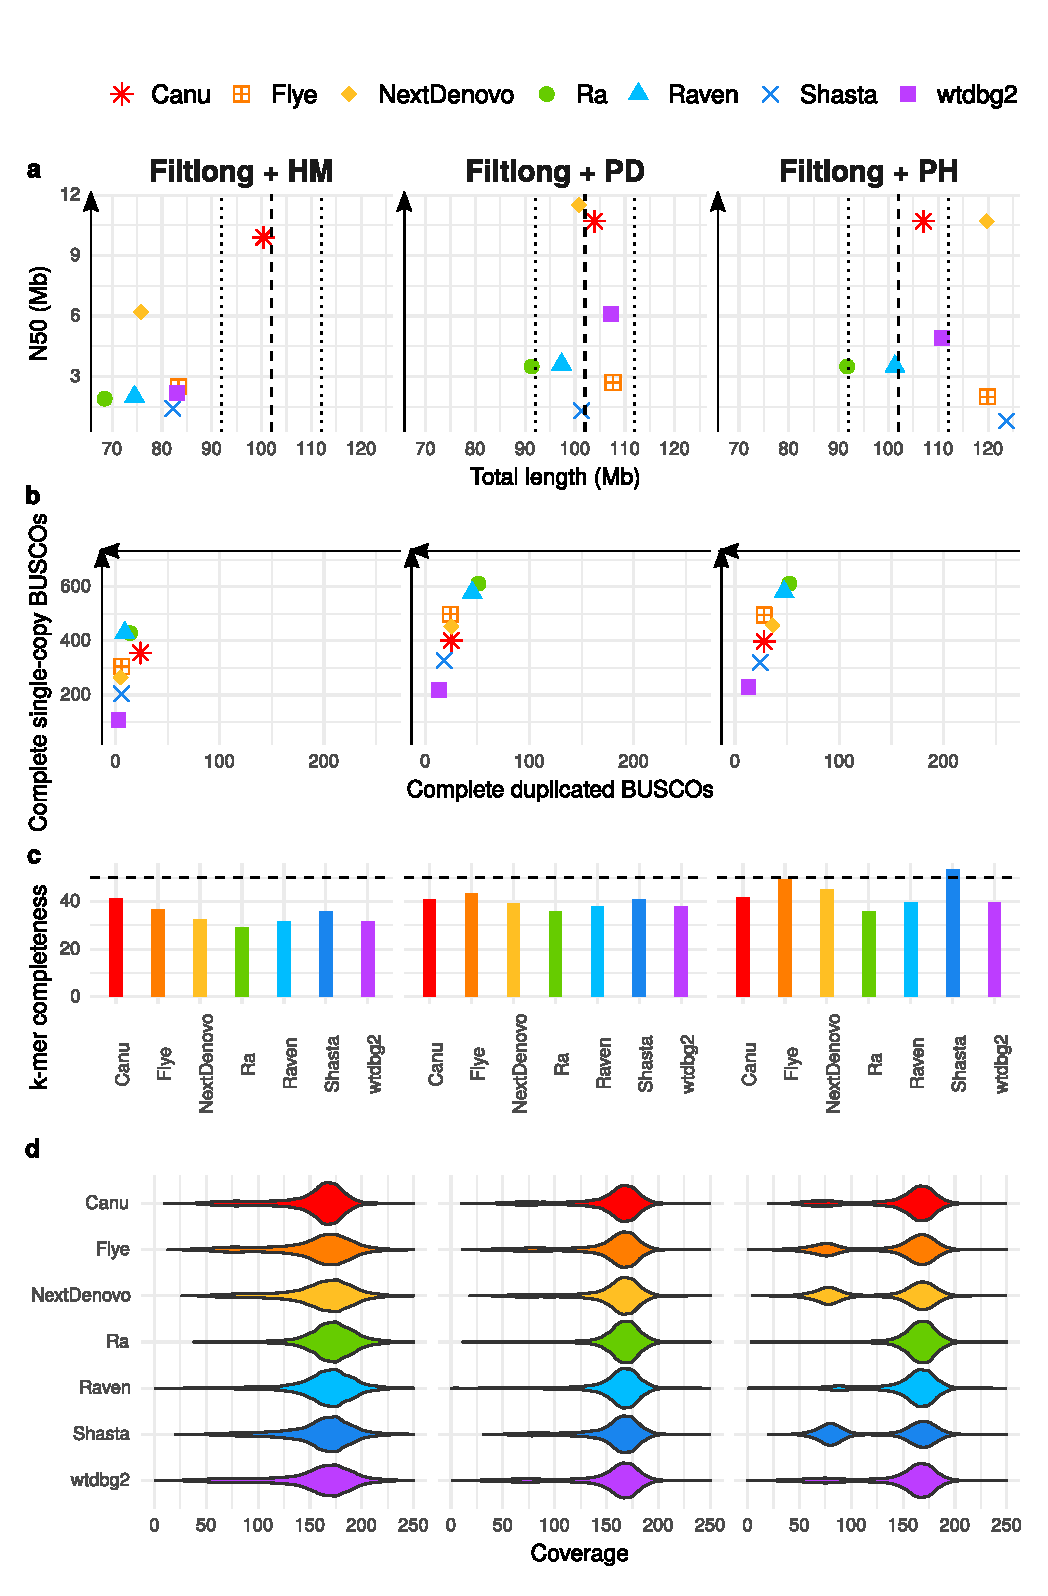
\includegraphics[width=13.5cm]{fig/benchmark/supp_nanopore_filtlong_purging_v20210310.eps}
   \caption{Statistics of Nanopore assemblies obtained from the Nanopore dataset filtered with Filtlong, with a subsequent removal of uncollapsed haplotypes with HaploMerger2 (HM), purge\_dups (PD), or purge\_haplotigs (PH). a) N50 plotted against total assembly length. The dashed line indicates the expected genome size, with a +/- 10 Mb margin delimited by the dotted lines. b) Number of complete single-copy BUSCOs plotted against number of complete duplicated BUSCOs, from a total of 954 orthologs. c) \textit{k}-mer completeness. The dashed line indicates the expected 50\% completeness. d) Long-read coverage distribution over the contigs.}
   \label{fig:nanopore_filtlong_purging}
 \end{figure}
 
   \begin{figure}[ht]
    \centering
     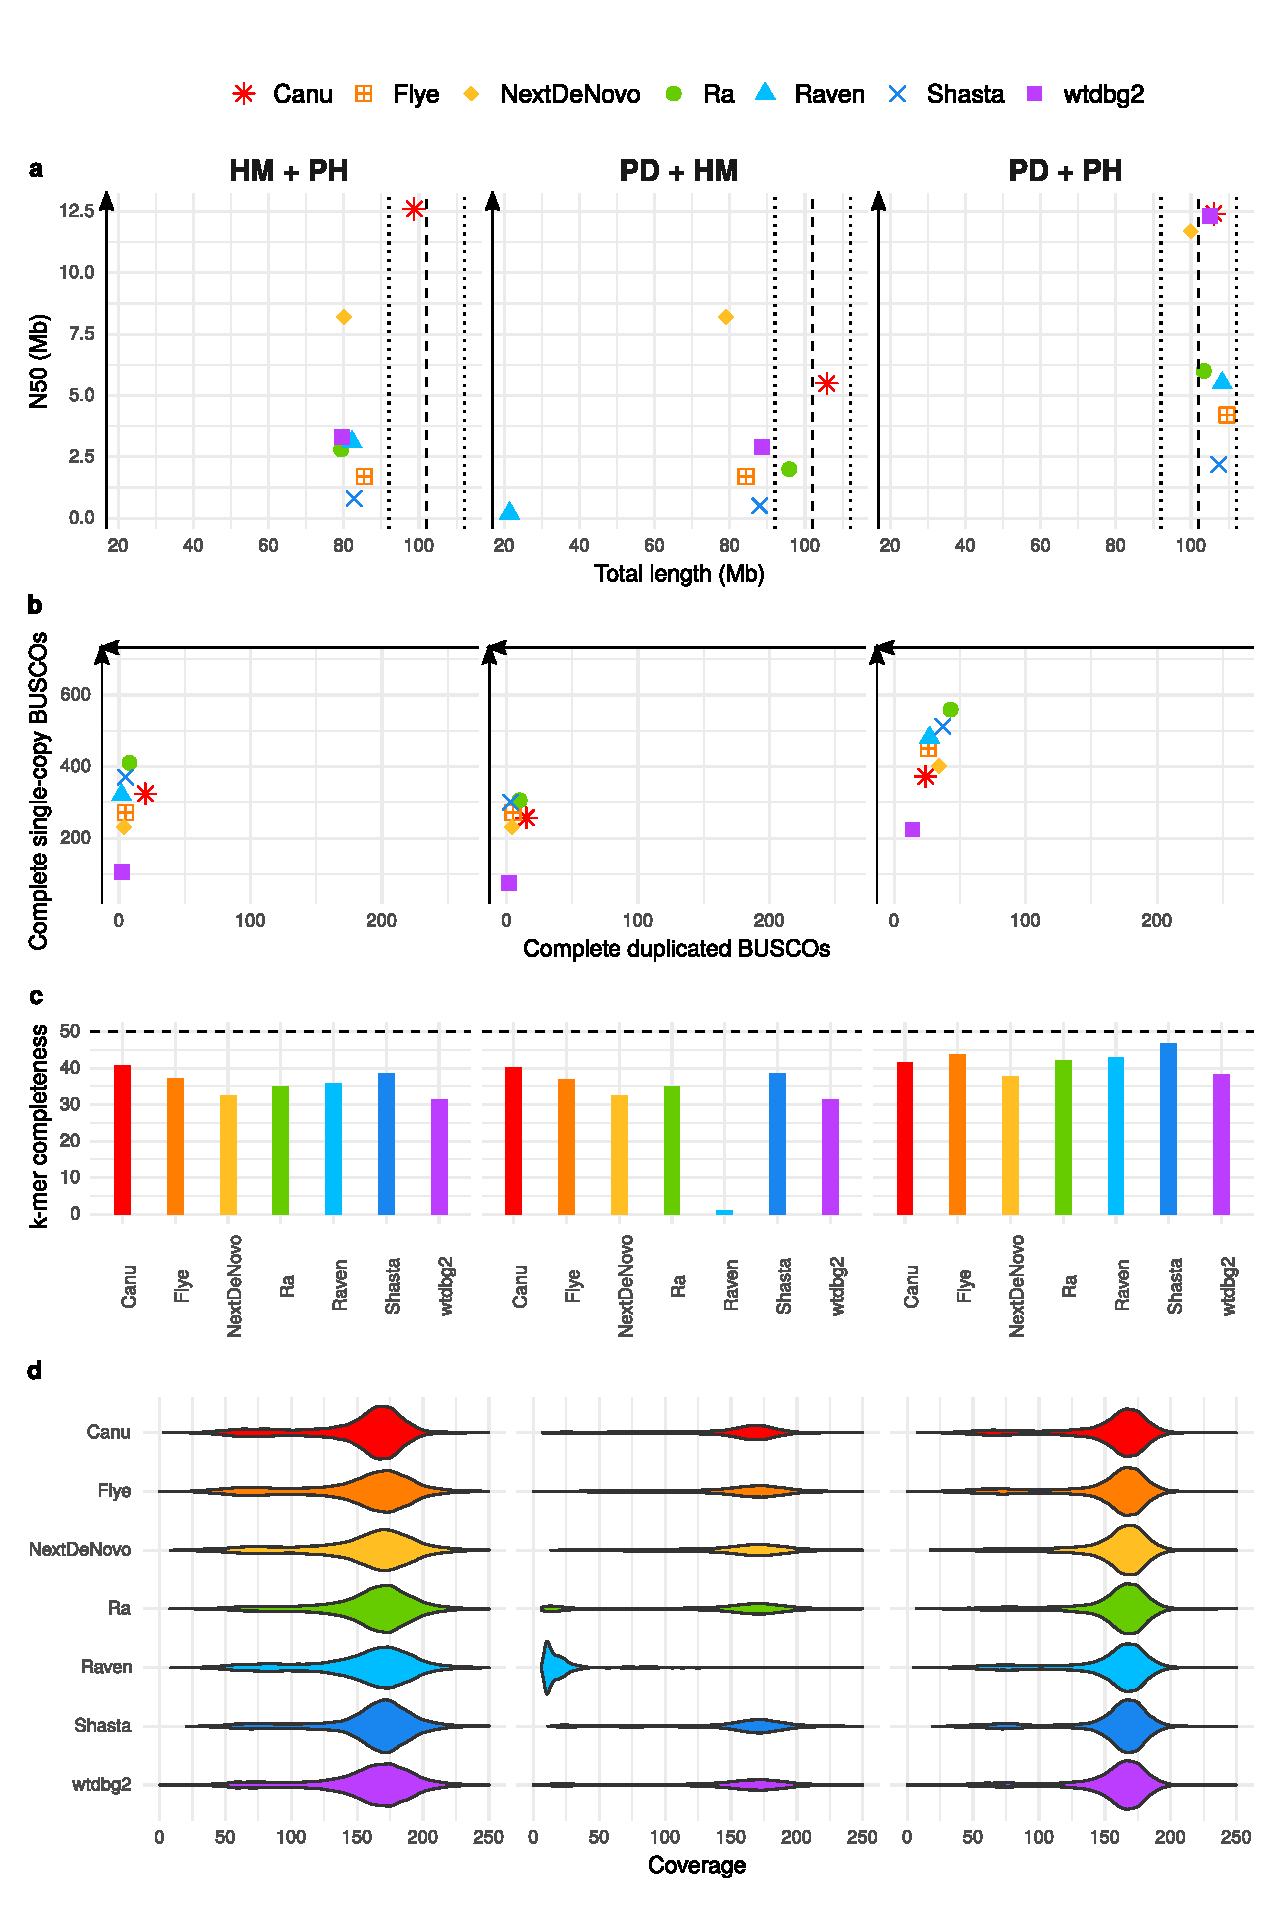
\includegraphics[width=13.5cm]{fig/benchmark/supp_nanopore_purging_combinations_v20200919.eps}
   \caption{Statistics of Nanopore assemblies obtained from the full Nanopore dataset with a subsequent removal of uncollapsed haplotypes with combinations of HaploMerger2 (HM), purge\_dups (PD), and purge\_haplotigs (PH). a) N50 plotted against total assembly length. The dashed line indicates the expected genome size, with a +/- 10 Mb margin delimited by the dotted lines. b) Number of complete single-copy BUSCOs plotted against number of complete duplicated BUSCOs, from a total of 954 orthologs. c) \textit{k}-mer completeness. The dashed line indicates the expected 50\% completeness. d) Long-read coverage distribution over the contigs.}
   \label{fig:nanopore_purging_combinations}
 \end{figure}
 
\begin{table}[ht]
\centering
\caption{Haploidy values computed by HapPy v0.1 for PacBio assemblies.}
\begin{adjustbox}{totalheight=\textheight-2\baselineskip}
\begin{tabular}{llc}
\hline
\textbf{Assembler} & \textbf{Processing} & \textbf{Haploidy} \\
\hline
Canu & raw assemblies & 0.59 \\
Flye & raw assemblies & 0.85 \\
NextDenovo & raw assemblies & 0.81 \\
Ra & raw assemblies & 0.90 \\
Raven & raw assemblies & 0.82 \\
Shasta & raw assemblies & 0.83 \\
wtdbg2 & raw assemblies & 0.90 \\
Canu & longest reads & 0.62 \\
Flye & longest reads & 0.85 \\
NextDenovo & longest reads & 0.94 \\
Ra & longest reads & 0.94 \\
Raven & longest reads & 0.88 \\
Shasta & longest reads & 0.96 \\
wtdbg2 & longest reads & 0.90 \\
Canu & Filtlong & 0.58 \\
Flye & Filtlong & 0.86 \\
NextDenovo & Filtlong & 0.88 \\
Ra & Filtlong & 0.94 \\
Raven & Filtlong & 0.90 \\
Shasta & Filtlong & 0.85 \\
wtdbg2 & Filtlong & 0.91 \\
Canu & HaploMerger2 & 0.84 \\
Flye & HaploMerger2 & 0.89 \\
NextDenovo & HaploMerger2 & 0.88 \\
Ra & HaploMerger2 & 0.92 \\
Raven & HaploMerger2 & 0.90 \\
Shasta & HaploMerger2 & 0.91 \\
wtdbg2 & HaploMerger2 & 0.92 \\
Canu & purge\_dups & 0.89 \\
Flye & purge\_dups & 0.89 \\
NextDenovo & purge\_dups & 0.90 \\
Ra & purge\_dups & 0.91 \\
Raven & purge\_dups & 0.90 \\
Shasta & purge\_dups & 0.90 \\
wtdbg2 & purge\_dups & 0.91 \\
Canu & purge\_haplotigs & 0.86 \\
Flye & purge\_haplotigs & 0.85 \\
NextDenovo & purge\_haplotigs & 0.87 \\
Ra & purge\_haplotigs & 0.88 \\
Raven & purge\_haplotigs & 0.80 \\
Shasta & purge\_haplotigs & 0.90 \\
wtdbg2 & purge\_haplotigs & 0.90 \\
\hline
\end{tabular}
\end{adjustbox}
\label{tab:pacbio_happy_part1}
\end{table}

\begin{table}[ht]
\centering
\caption{Haploidy values computed by HapPy v0.1 for PacBio assemblies.}
\begin{tabular}{llc}
\hline
\textbf{Assembler} & \textbf{Processing} & \textbf{Haploidy} \\
\hline
Canu & longest reads $+$ purge\_haplotigs & 0.87 \\ \
Flye & longest reads $+$ purge\_haplotigs & 0.85 \\
NextDenovo & longest reads $+$ purge\_haplotigs & 0.94 \\
Ra & longest reads $+$ purge\_haplotigs & 0.92 \\
Raven & longest reads $+$ purge\_haplotigs & 0.87 \\
Shasta & longest reads $+$ purge\_haplotigs & 0.96 \\
wtdbg2 & longest reads $+$ purge\_haplotigs & 0.90 \\
Canu & longest reads $+$ purge\_dups & 0.91 \\
Flye & longest reads $+$ purge\_dups & 0.90 \\
NextDenovo & longest reads $+$ purge\_dups & 0.97 \\
Ra & longest reads $+$ purge\_dups & 0.95 \\
Raven & longest reads $+$ purge\_dups & 0.91 \\
Shasta & longest reads $+$ purge\_dups & 0.97 \\
wtdbg2 & longest reads $+$ purge\_dups & 0.92 \\
Canu & Filtlong $+$ purge\_haplotigs & 0.56 \\ \
Flye & Filtlong $+$ purge\_haplotigs & 0.86 \\
NextDenovo & Filtlong $+$ purge\_haplotigs & 0.88 \\
Ra & Filtlong $+$ purge\_haplotigs & 0.93 \\
Raven & Filtlong $+$ purge\_haplotigs & 0.90 \\
Shasta & Filtlong $+$ purge\_haplotigs & 0.85 \\
wtdbg2 & Filtlong $+$ purge\_haplotigs & 0.94 \\
Canu & Filtlong $+$ purge\_dups & 0.90 \\
Flye & Filtlong $+$ purge\_dups & 0.90 \\
NextDenovo & Filtlong $+$ purge\_dups & 0.93 \\
Ra & Filtlong $+$ purge\_dups & 0.94 \\
Raven & Filtlong $+$ purge\_dups & 0.92 \\
Shasta & Filtlong $+$ purge\_dups & 0.92 \\
wtdbg2 & Filtlong $+$ purge\_dups & 0.91 \\
\hline
\end{tabular}
\label{tab:pacbio_happy_part2}
\end{table}

\begin{table}[ht]
\centering
\caption{Haploidy values computed by HapPy v0.1 for PacBio assemblies.}
\begin{tabular}{llc}
\hline
\textbf{Assembler} & \textbf{Processing} & \textbf{Haploidy} \\
\hline
Canu & HaploMerger2 $+$ purge\_haplotigs & 0.82 \\
Flye & HaploMerger2 $+$ purge\_haplotigs & 0.89 \\
NextDenovo & HaploMerger2 $+$ purge\_haplotigs & 0.88 \\
Ra & HaploMerger2 $+$ purge\_haplotigs & 0.88 \\
Raven & HaploMerger2 $+$ purge\_haplotigs & 0.83 \\
Shasta & HaploMerger2 $+$ purge\_haplotigs & 0.88 \\
wtdbg2 & HaploMerger2 $+$ purge\_haplotigs & 0.84 \\
Canu & purge\_dups $+$ HaploMerger2 & 0.91 \\
Flye & purge\_dups $+$ HaploMerger2 & 0.90 \\
NextDenovo & purge\_dups $+$ HaploMerger2 & 0.90 \\
Ra & purge\_dups $+$ HaploMerger2 & 0.92 \\
Raven & purge\_dups $+$ HaploMerger2 & 0.93 \\
Shasta & purge\_dups $+$ HaploMerger2 & 0.92 \\
wtdbg2 & purge\_dups $+$ HaploMerger2 & 0.92 \\
Canu & purge\_dups $+$ purge\_haplotigs & 0.88 \\
Flye & purge\_dups $+$ purge\_haplotigs & 0.89 \\
NextDenovo & purge\_dups $+$ purge\_haplotigs & 0.92 \\
Ra & purge\_dups $+$ purge\_haplotigs & 0.89 \\
Raven & purge\_dups $+$ purge\_haplotigs & 0.88 \\
Shasta & purge\_dups $+$ purge\_haplotigs & 0.90 \\
wtdbg2 & purge\_dups $+$ purge\_haplotigs & 0.91 \\
\hline
\end{tabular}
\label{tab:pacbio_happy_part3}
\end{table}

\begin{table}[ht]
\centering
\caption{Haploidy values computed by HapPy v0.1 for Nanopore assemblies.}
\begin{adjustbox}{totalheight=\textheight-2\baselineskip}
\begin{tabular}{llc}
\hline
\textbf{Assembler} & \textbf{Processing} & \textbf{Haploidy} \\
\hline
Canu & raw assemblies & 0.63 \\
Flye & raw assemblies & 0.79 \\
NextDenovo & raw assemblies & 0.72 \\
Ra & raw assemblies & 0.90 \\
Raven & raw assemblies & 0.83 \\
Shasta & raw assemblies & 0.86 \\
wtdbg2 & raw assemblies & 0.92 \\
Canu & longest reads & 0.59 \\
Flye & longest reads & 0.79 \\
NextDenovo & longest reads & 0.72 \\
Ra & longest reads & 0.95 \\
Raven & longest reads & 0.89 \\
Shasta & longest reads & 0.75 \\
wtdbg2 & longest reads & 0.92 \\
Canu & Filtlong & 0.67 \\
Flye & Filtlong & 0.81 \\
NextDenovo & Filtlong & 0.77 \\
Ra & Filtlong & 0.97 \\
Raven & Filtlong & 0.92 \\
Shasta & Filtlong & 0.72 \\
wtdbg2 & Filtlong & 0.87 \\
Canu & HaploMerger2 & 0.89 \\
Flye & HaploMerger2 & 0.87 \\
NextDenovo & HaploMerger2 & 0.89 \\
Ra & HaploMerger2 & 0.91 \\
Raven & HaploMerger2 & 0.88 \\
Shasta & HaploMerger2 & 0.90 \\
wtdbg2 & HaploMerger2 & 0.89 \\
Canu & purge\_dups & 0.92 \\
Flye & purge\_dups & 0.90 \\
NextDenovo & purge\_dups & 0.92 \\
Ra & purge\_dups & 0.93 \\
Raven & purge\_dups & 0.90 \\
Shasta & purge\_dups & 0.91 \\
wtdbg2 & purge\_dups & 0.93 \\
Canu & purge\_haplotigs & 0.86 \\
Flye & purge\_haplotigs & 0.79 \\
NextDenovo & purge\_haplotigs & 0.90 \\
Ra & purge\_haplotigs & 0.90 \\
Raven & purge\_haplotigs & 0.83 \\
Shasta & purge\_haplotigs & 0.86 \\
wtdbg2 & purge\_haplotigs & 0.91 \\
\hline
\end{tabular}
\end{adjustbox}
\label{tab:nanopore_happy_part1}
\end{table}

\begin{table}[ht]
\centering
\caption{Haploidy values computed by HapPy v0.1 for Nanopore assemblies.}
\begin{tabular}{llc}
\hline
\textbf{Assembler} & \textbf{Processing} & \textbf{Haploidy} \\
\hline
Canu & longest reads $+$ purge\_haplotigs & 0.85 \\
Flye & longest reads $+$ purge\_haplotigs & 0.79 \\
NextDenovo & longest reads $+$ purge\_haplotigs & 0.72 \\
Ra & longest reads $+$ purge\_haplotigs & 0.95 \\
Raven & longest reads $+$ purge\_haplotigs & 0.89 \\
Shasta & longest reads $+$ purge\_haplotigs & 0.75 \\
wtdbg2 & longest reads $+$ purge\_haplotigs & 0.91 \\
Canu & longest reads $+$ purge\_dups & 0.89 \\
Flye & longest reads $+$ purge\_dups & 0.91 \\
NextDenovo & longest reads $+$ purge\_dups & 0.95 \\
Ra & longest reads $+$ purge\_dups & 0.96 \\
Raven & longest reads $+$ purge\_dups & 0.95 \\
Shasta & longest reads $+$ purge\_dups & 0.93 \\
wtdbg2 & longest reads $+$ purge\_dups & 0.92 \\
Canu & Filtlong $+$ purge\_haplotigs & 0.90 \\
Flye & Filtlong $+$ purge\_haplotigs & 0.81 \\
NextDenovo & Filtlong $+$ purge\_haplotigs & 0.77 \\
Ra & Filtlong $+$ purge\_haplotigs & 0.97 \\
Raven & Filtlong $+$ purge\_haplotigs & 0.92 \\
Shasta & Filtlong $+$ purge\_haplotigs & 0.72 \\
wtdbg2 & Filtlong $+$ purge\_haplotigs & 0.89 \\
Canu & Filtlong $+$ purge\_dups & 0.93 \\
Flye & Filtlong $+$ purge\_dups & 0.91 \\
NextDenovo & Filtlong $+$ purge\_dups & 0.94 \\
Ra & Filtlong $+$ purge\_dups & 0.97 \\
Raven & Filtlong $+$ purge\_dups & 0.96 \\
Shasta & Filtlong $+$ purge\_dups & 0.94 \\
wtdbg2 & Filtlong $+$ purge\_dups & 0.91 \\
\hline
\end{tabular}
\label{tab:nanopore_happy_part2}
\end{table}

\begin{table}[ht]
\centering
\caption{Haploidy values computed by HapPy v0.1 for Nanopore assemblies.}
\begin{tabular}{llc}
\hline
\textbf{Assembler} & \textbf{Processing} & \textbf{Haploidy} \\
\hline
Canu & HaploMerger2 $+$ purge\_haplotigs & 0.89 \\
Flye & HaploMerger2 $+$ purge\_haplotigs & 0.87 \\
NextDenovo & HaploMerger2 $+$ purge\_haplotigs & 0.89 \\
Ra & HaploMerger2 $+$ purge\_haplotigs & 0.91 \\
Raven & HaploMerger2 $+$ purge\_haplotigs & 0.92 \\
Shasta & HaploMerger2 $+$ purge\_haplotigs & 0.90 \\
wtdbg2 & HaploMerger2 $+$ purge\_haplotigs & 0.90 \\
Canu & purge\_dups $+$ purge\_haplotigs & 0.91 \\
Flye & purge\_dups $+$ purge\_haplotigs & 0.90 \\
NextDenovo & purge\_dups $+$ purge\_haplotigs & 0.94 \\
Ra & purge\_dups $+$ purge\_haplotigs & 0.93 \\
Raven & purge\_dups $+$ purge\_haplotigs & 0.90 \\
Shasta & purge\_dups $+$ purge\_haplotigs & 0.91 \\
wtdbg2 & purge\_dups $+$ purge\_haplotigs & 0.92 \\
Canu & purge\_dups $+$ HaploMerger2 & 0.90 \\
Flye & purge\_dups $+$ HaploMerger2 & 0.88 \\
NextDenovo & purge\_dups $+$ HaploMerger2 & 0.90 \\
Ra & purge\_dups $+$ HaploMerger2 & 0.91 \\
Raven & purge\_dups $+$ HaploMerger2 & 0.51 \\
Shasta & purge\_dups $+$ HaploMerger2 & 0.90 \\
wtdbg2 & purge\_dups $+$ HaploMerger2 & 0.89 \\
\hline
\end{tabular}
\label{tab:nanopore_happy_part3}
\end{table}

\begin{table}[ht]
\centering
\caption{List of command lines used for each tool. Values L, M, H for \texttt{purge\_haplotigs cov} were selected for each assembly according to the histogram produced by \texttt{purge\_haplotigs hist}.}
\resizebox{\columnwidth}{!}{
\begin{tabular}{lll}
\hline
\textbf{Program} & \textbf{Dataset} & \textbf{Command lines} \\
\hline
Filtlong & - & \texttt{filtlong -{}-target\_bases 4092000000 -{}-mean\_q\_weight 10 long\_read\_data} \\
Canu & PacBio & \texttt{canu -d out -p out genomeSize=100m useGrid=false -pacbio-raw pb\_data} \\
Canu & Nanopore & \texttt{canu -d out -p out genomeSize=100m useGrid=false -nanopore-raw ont\_data}\\
Flye & PacBio & \texttt{flye -o out -g 100m -{}-pacbio-raw pb\_data} \\
Flye & Nanopore & \texttt{flye -o out -g 100m -{}-nano-raw ont\_data} \\
NextDenovo & PacBio & \texttt{echo pb\_data $>$ input.fofn} \\
 &  & \texttt{seq\_stat input.fofn -g 100Mb -d 150 $>$ stats.txt} \\
 &  & \texttt{NextDenovo run.cfg} \\
NextDenovo & Nanopore & \texttt{echo ont\_data $>$ input.fofn} \\
 &  & \texttt{seq\_stat input.fofn -g 100Mb -d 150 $>$ stats.txt} \\
 &  & \texttt{NextDenovo run.cfg} \\
Ra & PacBio & \texttt{ra -x pb pb\_data $>$ assembly.fasta}\\
Ra & Nanopore & \texttt{ra -x ont ont\_data $>$ assembly.fasta}\\
Raven & - & \texttt{raven long\_read\_data $>$ assembly.fasta}\\
Shasta & PacBio & \texttt{shasta -{}-input pb\_data -{}-Reads.minReadLength 0 -{}-assemblyDirectory out -{}-Assembly.consensusCaller Modal -{}-Kmers.k 12} \\
Shasta & Nanopore & \texttt{shasta -{}-input ont\_data -{}-Reads.minReadLength 0 -{}-assemblyDirectory out} \\
wtdbg2 & PacBio & \texttt{wtdbg2 -x rs -g 100m -i pb\_data -fo out} \\
    & & \texttt{wtpoa-cns -i out.ctg.lay.gz -o out.ctg.fa} \\
    & & \texttt{minimap2 -x map-pb -a out.ctg.fa pb\_data | samtools sort $>$ out.ctg.bam} \\
    & & \texttt{samtools view out.ctg.bam | wtpoa-cns -d out.ctg.fa -i - -fo assembly.fasta} \\
wtdbg2 & Nanopore & \texttt{wtdbg2 -x ont -g 100m -i ont\_data -fo out} \\
    & & \texttt{wtpoa-cns -i out.ctg.lay.gz -o out.ctg.fa} \\
    & & \texttt{minimap2 -x map-ont -a out.ctg.fa ont\_data | samtools sort $>$ out.ctg.bam} \\
    & & \texttt{samtools view out.ctg.bam | wtpoa-cns -d out.ctg.fa -i - -fo assembly.fasta} \\
HaploMerger2 & - & \texttt{samtools faidx assembly.fasta} \\
 &  & \texttt{BuildDatabase -name asm.db -engine ncbi assembly.fasta} \\
 &  & \texttt{RepeatModeler -engine ncbi -database asm.db} \\
  &  & \texttt{RepeatMasker -e ncbi -lib consensi.fa -xsmall assembly.fasta} \\
  &  & \texttt{run\_all.batch} \\
purge\_dups & PacBio & \texttt{echo pb\_data $>$ input.fofn} \\ 
 &  & \texttt{pd\_config.py assembly.fasta input.fofn} \\ 
 &  & \texttt{run\_purge\_dups.py config.json purge\_dups\_bin species\_id} \\ 
purge\_dups & Nanopore & \texttt{echo ont\_data $>$ input.fofn} \\ 
 &  & \texttt{pd\_config.py assembly.fasta input.fofn} \\ 
 &  & \texttt{run\_purge\_dups.py config.json purge\_dups\_bin species\_id} \\ 
purge\_haplotigs & PacBio & \texttt{minimap2 -ax map-pb assembly.fasta pb\_data -{}-secondary$=$no $>$ aligned.bam} \\
    & & \texttt{samtools sort -o ali.sorted.bam -T tmp.ali aligned.bam} \\
    & & \texttt{samtools index ali.sorted.bam} \\
    & & \texttt{samtools faidx assembly.fasta} \\
    & & \texttt{purge\_haplotigs hist -b ali.sorted.bam -g assembly.fasta} \\
    & & \texttt{purge\_haplotigs cov -i ali.sorted.bam -l L -m M -h H -o cov\_stats.csv}\\
    & & \texttt{purge\_haplotigs purge -g assembly.fasta -c cov\_stats.csv -o assembly.purged.fasta}\\
purge\_haplotigs & Nanopore & \texttt{minimap2 -ax map-ont assembly.fasta ont\_data -{}-secondary$=$no $>$ aligned.bam}\\
    & & \texttt{samtools sort -o ali.sorted.bam -T tmp.ali aligned.bam} \\
    & & \texttt{samtools index ali.sorted.bam} \\
    & & \texttt{samtools faidx assembly.fasta} \\
    & & \texttt{purge\_haplotigs hist -b ali.sorted.bam -g assembly.fasta} \\
    & & \texttt{purge\_haplotigs cov -i ali.sorted.bam -l L -m M -h H -o cov\_stats.csv}\\
    & & \texttt{purge\_haplotigs purge -g assembly.fasta -c cov\_stats.csv -o assembly.purged.fasta}\\
BBtools & - & \texttt{reformat.sh in=long\_reads\_data out=subset\_data samplebasestarget=number\_of\_bases} \\
BUSCO & - & \texttt{busco -i assembly.fasta -o busco\_output -l metazoa\_odb10 -m genome} \\
KAT & Illumina & \texttt{kat comp -o kat\_output 'end1.fastq end2.fastq' assembly.fasta} \\
tinycov & Nanopore & \texttt{minimap2 -x map-ont -a assembly.fasta ont\_data | samtools sort $>$ aligned.bam} \\
    & & \texttt{tinycov covplot -r 20000 -t cov.txt aligned.bam} \\
tinycov & PacBio & \texttt{minimap2 -x map-pb -a assembly.fasta pb\_data | samtools sort $>$ aligned.bam} \\
    & & \texttt{tinycov covplot -r 20000 -t cov.txt aligned.bam} \\
HapPy & Nanopore & \texttt{minimap2 -x map-ont -a assembly.fasta ont\_data | samtools sort $>$ aligned.bam} \\
    & & \texttt{HapPy.py depth aligned.bam out\_dir} \\
    & & \texttt{HapPy.py estimate out\_dir/aligned.bam.hist} \\
HapPy & PacBio & \texttt{minimap2 -x map-pb -a assembly.fasta pb\_data | samtools sort $>$ aligned.bam} \\
    & & \texttt{HapPy.py depth aligned.bam out\_dir} \\
    & & \texttt{HapPy.py estimate out\_dir/aligned.bam.hist} \\
time & - & \texttt{/usr/bin/time -v -o time\_output.txt}\\
\hline
\end{tabular}
}
\label{tab:command_lines}
\end{table}

\begin{table}[ht]
\centering
\caption{Long-read and short-read datasets used in the study.}
\begin{tabular}{lccc}
\hline
\textbf{Data type} & \textbf{Minimum length} & \textbf{Total data} & \textbf{N50} \\
\hline
PacBio & - & 23.5 Gb & 11.6 kb \\
& 15 kb & 4.7 Gb & 17.6 kb \\
\hline
Nanopore & - & 17.5 Gb & 18.8 kb  \\
& 30 kb & 5.7 Gb & 51.8 kb  \\
\hline
Illumina 2*250 bp & 30 bp & 11.4 Gb & 250 bp \\
\hline
\end{tabular}
\label{tab:datasets}
\end{table}